%
% Modelo para relat￳rio da disciplina de Projecto de Engenharia Informatica
% do MEI.
%
% Incorpora elementos impostos pelo Regulamento de Estudos Pos-Graduados da
% Universidade de Lisboa (Deliberacao 1506/2006 - Diario da Repblica, 2.a s←rie 
% - n.o 209 - 30 de Outubro de 2006)
%
\documentclass[12pt,openright,twoside]{report}
\usepackage[show]{chato-notes}
\usepackage[utf8]{inputenc}
% Quem tiver problemas com os acentos, trocar utf8 por latin1

%\usepackage{setspace}
\usepackage[portuguese,english]{babel}

\usepackage{times}
\usepackage[hyphens]{url}
%\usepackage{url}
\usepackage{graphicx}
\usepackage{mdwlist}
\usepackage[nottoc]{tocbibind}
\usepackage{csquotes}
\usepackage{listings}
\usepackage[table,hyperref,x11names]{xcolor}
\usepackage{array,booktabs}
\usepackage{multirow}
\usepackage{mathrsfs}
\usepackage{dialogue}
%To get figures and tables side by side
\usepackage{floatrow}
\newfloatcommand{capbtabbox}{table}[][\FBwidth]
% end figures and tables side by side



%%%%%%%%%%%%%%%%%%%%%%%
%title 
\makeatletter
\renewcommand{\@makechapterhead}[1]{%
\vspace*{50 pt}%
{\setlength{\parindent}{0pt} \raggedright \normalfont
\bfseries\Huge
\ifnum \value{secnumdepth}>1 
   \if@mainmatter Chapter \thechapter\ --\ \fi%
\fi
#1\par\nobreak\vspace{40 pt}}}
\makeatother


%%%%%%%%%%%%%%%%%%%%%%%%%%
%footnote in tables 
\usepackage{threeparttable}
%end footnote in tables

% Indice remissivo
\usepackage{makeidx}
\makeindex

%%%%%%%%%%%%%%%%%% BIG O 
\usepackage{amsmath}
\newcommand{\BigO}[1]{\ensuremath{\operatorname{O}\bigl(#1\bigr)}}
%%%%%%%%%%%%%% BIG O
%quotes
\usepackage{epigraph}
\usepackage{attrib}
\usepackage{titlesec}
\usepackage{ amssymb }

%\titlespacing{\subsubsection}{0pt}{0pt}{0pt}
%\titleformat{\subsubsection}[runin]{\normalfont\bfseries}{\thesubsection.}{3pt}{}


\usepackage[nomain,acronym,xindy,nonumberlist]{glossaries}
\usepackage{glossary-mcols}  
\renewcommand*{\glsmcols}{3}  
\glossarystyle{mcolindex}
\newacronym{sdn}{SDN}{Software Defined Network}

\newacronym{nib}{NIB}{Network Information Base}

\newacronym{wan}{WAN}{Wide Area Network}

\newacronym{nos}{NOS}{Network Operating System}

\newacronym{os}{OS}{Operating System}

\newacronym{onf}{ONF}{Open Network Foundation}

\newacronym{of}{OF}{OpenFlow}

\newacronym{fifo}{FIFO}{First In,First Out}

\newacronym{smr}{SMR}{State Machine Replication}

\newacronym{arp}{ARP}{Address Resolution Protocol}
\newacronym{api}{API}{Application Programming Interface}
\newacronym{lru}{LRU}{Least Recently Used} 
\newacronym{ip}{IP}{Internet Protocol}
\newacronym{icmp}{ICMP}{Internet Control Message Protocol} 
\newacronym{ipv6}{IPv6}{Internet Protocol version 6}
\newacronym{vlan}{VLAN}{Virtual Local Area Network} 
\newacronym{mac}{MAC}{Media Access Control}


\newacronym{rest}{REST}{Representational State Transfer} 
\newacronym{vip}{VIP}{Virtual Enpoint Internet Protocol} 
\newacronym{rpc}{RPC}{Remote Procedure Call} 
\newacronym{sql}{SQL}{Structured Query Language} 

\newacronym{tcp}{TCP}{Transmission Control Protocol}
\newacronym{rcp}{RCP}{Routing Control Platform}
\newacronym{bgp}{BGP}{Border Gateway Protocol}
\newacronym{as}{AS}{Autonomous System}
\newacronym{ibgp}{iBGP}{interior Border Gateway Protocol}
\newacronym{url}{URL}{Uniform Resource Locator}
\newacronym{dhcp}{DHCP}{Dynamic Host Configuration Protocol}
\newacronym{http}{HTTP}{HyperText Transport Protocol} 
\makeglossary  

% Links
\usepackage{hyperref}

% Package para cabecalhos
\usepackage{fancyhdr}
\usepackage{lastpage}

\usepackage[font={small}]{caption}
\usepackage{subcaption}
\usepackage[style=numeric-comp, sorting=none,  isbn=false,
url=false, doi=false, eprint=false,backref=true]{biblatex}

%%%%%%%%%%%
\newbibmacro*{bbx:parunit}{%
  \ifbibliography
    {\setunit{\bibpagerefpunct}\newblock
     \usebibmacro{pageref}%
     \clearlist{pageref}%
     \setunit{\adddot\par\nobreak}}
    {}}

\renewbibmacro*{doi+eprint+url}{%
  \usebibmacro{bbx:parunit}% Added
  \iftoggle{bbx:doi}
    {\printfield{doi}}
    {}%
  \iftoggle{bbx:eprint}
    {\usebibmacro{eprint}}
    {}%
  \iftoggle{bbx:url}
    {\usebibmacro{url+urldate}}
    {}}

\renewbibmacro*{eprint}{%
  \usebibmacro{bbx:parunit}% Added
  \iffieldundef{eprinttype}
    {\printfield{eprint}}
    {\printfield[eprint:\strfield{eprinttype}]{eprint}}}

\renewbibmacro*{url+urldate}{%
  \usebibmacro{bbx:parunit}% Added
  \printfield{url}%
  \iffieldundef{urlyear}
    {}
    {\setunit*{\addspace}%
     \printtext[urldate]{\printurldate}}}

%%%%%%%%%%%%%
\bibliography{bibliografia}
\fancyhf{} %
\lhead{\nouppercase {\leftmark}} %
\rhead{\nouppercase {\bf \thepage}}
\renewcommand{\headrulewidth}{0.1pt}
%%%%%%%%%%%
\usepackage{titletoc}

%%%%%%%%%
%%%%
%colouring tables
\usepackage{color, colortbl}
\definecolor{Gray}{gray}{0.9}
\definecolor{LightCyan}{rgb}{0.88,1,1}
%%%%%%%%

%%%%%%%%%%%

\hyphenation{protocol}

\newcommand{\etal}{et al.}

%%%%%%%%%%%%%%%%%%%%


% Comando para inserir pagina em branco (inserida na numeracao, mas sem
% numero impresso) para quando e' preciso obrigar um capitulo a comecar
% do lado direito (pagina impar)
\newcommand{\LIMPA}{
\newpage
\mbox{}
\thispagestyle{empty}
}

% Igual, mas insere pagina com numero impresso (normalmente nao se usa)
\newcommand{\LIMPAC}{
\newpage
\mbox{}
\thispagestyle{plain}
}

%%%%%%%%%
% \renewcommand{\epigraphrule}{0pt}
\setlength{\epigraphwidth}{0.6\textwidth}
% \renewcommand{\textflush}{flushepinormal}
% \makeatletter
% % Taken and updated from http://mirrors.ctan.org/macros/latex/contrib/epigraph/epigraph.dtx
% \renewcommand{\@epitext}[1]{%
%   \begin{minipage}{\epigraphwidth}\begin{\textflush} \hspace*{20pt}\emph{#1}\\
%     \ifdim\epigraphrule>\z@ \@epirule \else \vspace*{-.5\baselineskip} \fi
%   \end{\textflush}\end{minipage}}
% \makeatother
%%%%%%%%%%%%%%%%%%%%


%%%%%%%%%%%%%
%%%%%%% PERSONAL COMMANDS %%%%%%%%%%%
\newcommand{\distcontrollers}{\cite{Tootoonchian:2010vy,Koponen:2010th,Yeganeh:2012jm,jain2013b4}}
\newcommand{\distcontrollerspaper}{\cite{Tootoonchian:2010vy, Koponen:2010th,Yeganeh:2012jm}}
%END 

\newcommand{\tbl}[2]{\begin{tabular}{#1}#2\end{tabular}}
\newcommand{\ml}[2]{#1 $\pm$ #2} 

%
% ALTERAR AQUI AS INFORMACOES RELATIVAS AO PROJECTO
%
\newcommand{\PEITITULO}{A Consistent and Fault-Tolerant Data Store for Software Defined Networks}
\newcommand{\PEIAutor}{Fábio Andrade Botelho}
\newcommand{\PEIAutorNumAluno}{41625}

%Orientador e CoOrientador *sem* titulos (e.g. Prof. Doutor)
\newcommand{\PEIOrientador}{Alysson Neves Bessani}
\newcommand{\PEICoOrientador}{Fernando Manuel Valente Ramos} %se nao se aplicar, nao importa o que aqui esteja

%Se aplicavel, o supervisor pode ter um titulo (Dr., Eng.) colocado aqui
\newcommand{\PEISupervisorInstituicao}{Nome Completo do Supervisor}  %se nao se aplicar, nao importa o que aqui esteja

\newcommand{\PEIAnoLectivo}{2012/2013}
\newcommand{\PEIAno}{2013}

% Comentar/descomentar conforme conveniente
\newcommand{\PEITIPO}{DISSERTA\c{C}\~{A}O }
%\newcommand{\PEITIPO}{PROJECTO }

% Comentar/descomentar conforme conveniente
%\newcommand{\PEIIdiomaTese}{\selectlanguage{portuguese}}
\newcommand{\PEIIdiomaTese}{\selectlanguage{english}}

% Comentar/descomentar conforme conveniente
%\newcommand{\MEIEspecializacao}{Segurança Informática}
%\newcommand{\MEIEspecializacao}{Arquitectura, Sistemas e Redes de Computadores}
%\newcommand{\MEIEspecializacao}{Interac��o e Conhecimento}
%\newcommand{\MEIEspecializacao}{Engenharia de Software }

\usepackage{ifpdf}
\ifpdf
\pdfinfo {
	/Author (\PEIAutor)
	/Title (Projecto em Segurança Informatica)
	/Subject (Segurança Informatica)
	/Keywords (state machine replication, software defined networks)
	/CreationDate (D:20100510104905)
}
\fi

\usepackage[dvips]{geometry}
\geometry{a4paper=true,portrait=true,left=3cm,right=3cm,top=2.5cm,bottom=3.5cm}

\title{\PEITITULO}
\author{\PEIAutor}
%\date{\today}

\begin{document}

%\doublespacing

%Capa e pagina de rosto
\selectlanguage{portuguese}

\pagestyle{empty}

% ----------------------------------------------------------------------
% Capa
\begin{center}
\vspace{3cm}\normalfont\normalfont
\textsc{\huge{Universidade de Lisboa}}\\
\LARGE{Faculdade de Ci\^{e}ncias}\\
\Large{Departamento de Inform\'{a}tica}\\
\vspace{1cm}
\includegraphics[scale=.3]{pic/logo_ul.jpg}\\
%\includegraphics[scale=.6]{pic/logo_fcul.jpg}\\

\vspace{2cm}
\PEIIdiomaTese
\Large{\bf \PEITITULO}\\
\selectlanguage{portuguese}
\vspace{1cm}
%projecto realizado na\\
\vspace{0.7cm}
%\Large{\bf Nome da Instituicao de Acolhimento}\\
%\vspace{0.7cm}
%por\\
\vspace{0.7cm}
\Large{\bf \PEIAutor}\\
\vspace{2.4cm}
\Large{\bf \PEITIPO}\\
\vfill
\Large{MESTRADO EM SEGURANÇA  INFORM\'{A}TICA}\\

\vfill
\PEIAno

\end{center}
\newpage
\mbox{}
\newpage
% Fim da capa
% ----------------------------------------------------------------------

\setcounter{page}{1}
\pagenumbering{roman}

% ----------------------------------------------------------------------
% Folha de Rosto

\begin{center}
\vspace{3cm}\normalfont\normalfont
\textsc{\huge{Universidade de Lisboa}}\\
\LARGE{Faculdade de Ci\^{e}ncias}\\
\Large{Departamento de Inform\'{a}tica}\\
\vspace{0.9cm}
\includegraphics[scale=.3]{pic/logo_ul.jpg}\\
%\includegraphics[scale=.6]{pic/logo_fcul.jpg}\\
\vspace{1.9cm}
\PEIIdiomaTese
\Large{\bf \PEITITULO}\\
\selectlanguage{portuguese}
\vspace{1.4 cm}
\Large{\bf \PEIAutor}\\
%\vspace{2.4cm}
\vspace{1.9 cm}
\Large{\bf \PEITIPO}\\
\end{center}
\vspace{0.4 cm}
\begin{center}
\Large{MESTRADO EM SEGURANÇA INFORM\'{A}TICA}\\

\end{center}
\vspace{1 cm}
Disserta\c{c}\~{a}o orientada pelo Prof. Doutor \PEIOrientador \\
% DESCOMENTAR a linha relevante (se alguma), removendo o % no inicio
e co-orientado pelo Prof. Doutor \PEICoOrientador \\
%e por \PEISupervisorInstituicao
%\vfill
\vspace{-0.2cm} 
\begin{center}
\large\PEIAno
\end{center}
\newpage
\thispagestyle{empty}
\mbox{}
\newpage
% Fim da Folha de rosto
% ----------------------------------------------------------------------


% Agradecimentos
\pagestyle{plain}

\vspace*{2cm}
\begin{center}
\selectlanguage{portuguese}
\Large \bf Agradecimentos
%\selectlanguage{english}
%\Large \bf Acknowledgments
\end{center}
\vspace*{1cm} \setlength{\baselineskip}{0.6cm}
Aos meus orientadores --- Prof. Doutor Alysson Neves Bessani, Prof. Doutor Fernando Manuel Valente Ramos Doutor, e  Diego Kreutz, que mais do ocuparem titulos e posições tomaram lugar numa activa equipa de trabalho que tornou este projecto possivel. 
Um muito obrigado por toda a paciência, apoio, e confiança ao longo do meu último ano. 
No contexto do meu percurso na FCUL queria também agradecer ao Prof. Doutor Hugo Alexandre Tavares Miranda, que muito me ensinou sobre sistemas distribuídos, e também aos companheiros do laboratório 25 que muito me ensinaram e desafiaram. Este grupo de pessoas constitui o grupo de  pessoas mais inteligentes  e trabalhadoras que já tive oportunidade de conhecer. 
Queria agradecer também aos reviewers da EWSDN pelos comentários que ajudaram a melhorar o paper que foi resultado deste trabalho. Além disso queria agradacer ao financiamento que foi parcialmente supportado pelo EC FP7 através do projecto BiobankCloud (ICT-317871) e também pela FCT através do programa Multi-anual do LASIGE. 

No hemisférico pessoal queria agradecer a todos os que me carregaram até aqui. Nomeadamente a minha familia (pais e irmas), que mais do que ser familia, acreditou em mim, e levou-me às costas todos anos. Eu nunca vos vou conseguir retribuir o quanto fizeram por mim. 
De seguida à minha  companheira de viagem, Maria Lalanda, por me acompanhar nesta jornada comprida. Foste o melhor deste caminho, espero no futuro perder-me apenas contigo. 

De restante queria agradecer a uma grande lista de pessoas e coisas. Em especial: 
Ao pessoal do Jardim, pelas baldas, pelo jardim, por todo o tempo envoltos em ritmo e poesia. São demasiados os nomes para referir aqui, mas não podia deixar de referir as pessoas que mais me apoiaram neste percurso: João Sardinha, e Tâmara Andrade. 
Em Braga, à Catarina e Filipe Rebelo, e à senhora Eleanor por terem acreditado em mim.  Ao Manuel Barbosa por me alavancar, e ao  José Silva e à Barbara Manso por se infiltrarem na minha casa. Voçês três são familia (e a Conceição veio por arrasto :). Um especial agradecimento ao José, por ser o meu primeiro companheiro de batalha numa guerra bem complicada. Nunca é tarde para apanhar o comboio Cacilda! Aos Monads, à casa vintage, ao gadgets do Toxa, à bandeira que soprava na direcção de casa, e a todo o restante foklore. Ao JBB e JNO por inspirarem. 

%Sinto que estive muito acquém do que devido, por mais esforço que tenha colocado neste projecto. 
%Espero ter aprendido com os erros, e espero que no restante processo desse trabalho, possa-vos supreender com mais e melhor. 
%Também quero agradecer por ao prof. Alysson por me ter ensinado o \\vspace (prometo não sobre-utilizar :) e ao prof Fernando Ramos por me ter vendido o meu proprio peixe. 

Em Lisboa, à Filipa Costa e João Pereira, aos concertos e aos shots por suportarem o gajo mais chato de sempre. 
Ao MSI por ter me confrontado  com o maior desafio da minha vida. 
Ao José Lopes, porque sem ele nunca teria conseguido. Mesmo que conseguisse, não teria piada. Fico à espera que me ``faças um turing'' rapaz. 
Ao pessoal do FCUL que muito ajudou. Em especial o Emanuel, Juliana e Anderson. 
À RUMO que me acolheu. Com remorso não tive o impulso de explorar os teus cantos. 

Finalmente a todas as máquinas automáticas do c* que me alimentaram durante as semanas do Globox, ao café, SG Ventil, stack-overflow e lego-coding: um muito obrigado. Ao Lamport por usar t-shirts em apresentações, inventar o LaTeX e um zilião de papers. 
Por fim ao Charlie, ``who has always made it out of the jungle!''. Mesmo sem cão!\\ 

\emph{À Lonjura, ao Insularismo e  à Ilha!} \\



\LIMPA
\LIMPA

~
\vfill

\selectlanguage{portuguese}
%\selectlanguage{english}
\begin{flushright}\textit{A todos ``os meus conhecidos''  que já levaram porrada. }\end{flushright}

\LIMPA

%%% Local Variables: 
%%% mode: latex
%%% TeX-master: "../PEI"
%%% End: 


% Pagina do resumo em portugues
%\pagestyle{empty}

% ----------------------------------------------------------------------
% P�gina do resumo em Portugu�s:
\selectlanguage{portuguese}
\vspace*{2cm}
\begin{center} \Large \bf Resumo
\end{center}
\vspace*{1cm} \setlength{\baselineskip}{0.6cm}
\todo{Ignore...}
O sucesso da Internet é indiscutível. No entanto desde à muito tempo
que são feitas sérias críticas à sua arquitectura. 
Investigadores acreditam que o principal
problema reside no facto de os dispositivos de rede incorporarem 
funções distintas e complexas que vão além do objectivo de encaminhar pacotes para o qual foram criados. O melhor exemplo, são os protocolos distribuidos complexos que tanto os \emph{routers} como os \emph{switches} precisam de executar para as redes funcionarem correctamente. De forma a resolver este problema
uma arquitetura de rede diferente tem vindo a ser adoptada 
 tanto pela comunidade científica como pela indústria. Nestas novas redes, conhecidas como  \emph{Software Defined Networks} (SDN), há uma separação física entre o plano de controlo do plano de dados. Isto é, toda a lógica e estado de controlo da rede  é retirada dos dispositivos de rede, para passar a ser executada num \emph{controlador} \emph{logicamente} centralizado que com um visão global, lógica e coerente da rede, consegue controlar a mesma de forma dinâmica. Com esta delegação de funções para o controlador os dispositivos de rede podem dedicar-se exclusivamente à sua função essencial de encaminhar pacotes de dados. 
Embora existam controladores centralizados que escalam a milhares de \emph{hosts} há a necessidade de os tornar distribuido de forma a conseguir suportar a escala de \emph{data-centers} e redes modernas. No entanto a distribuição introduz vários desafios devido aos ambiente heterogêneo, assíncrono e faltoso onde os controladores necessariamente operam. 
Atualmente, os controladores de SDN distríbuidos utilizam modelos de distribuição não transparentes, com propriedades fracas como coerência futura que exigem maior cuidado no desenvolvimento de aplicações de controlo de rede no controlador. Isto deve-se à ideia mal-formada de que propriedades como coerência forte impedem a escalabilidade do controlador. 
O nosso trabalho irá contribuir com estudo e desenvolvimento dum controlador distribuido com coerência forte e tolerante a faltas para SDN. Este será conseguido com recurso a técnicas bem conhecidas de replicação baseada na máquina de estados distribuida. Um controlador com coerência forte traduz-se num modelo de programação mais simples e transparente à distribuição do controlador. Além disto, acreditámos que mesmo apresentando a propriedade de coerência forte, o nosso controlador irá conseguir apresentar uma performance superior à dos existentes na literatura. 

\todo{Pelo menos 1200 palavras} 
\vfill

\begin{flushleft}
\textbf{Palavras-chave:}
Replicação, Coerência Forte, Redes Controladas por Software, Tolerância a
Faltas, Máquina de Estados Distribuída, Plano de Controlo Distribuído. 
\end{flushleft}

\LIMPA
% Fim da p�gina do resumo em Portugu�s
% ----------------------------------------------------------------------


% Pagina do resumo em ingles
% ----------------------------------------------------------------------
% P�gina do resumo em Ingl�s:
\selectlanguage{english}
\vspace*{2cm}
\begin{center}
\Large \bf Abstract
\end{center}
\vspace*{1cm} \setlength{\baselineskip}{0.6cm}

This work is motivated by the 
emergent network architecture of Software
Defined Networks where the control of the network is extracted from the
network devices and delegated to a
server named controller that is responsible for dynamically
configuring the network devices present in the infrastructure. The
controller has the advantage of logically centralizing the network
state in contrast to the previous model where state was distributed
across the network devices. If spite of this logical centralization,
the control plane (where the controller operates)  must be distributed
in order to support the scale of modern datacenters and
networks. However, this distribution introduces several challenges due
to the heterogeneous, asynchronous and faulty environment where the
controller operates. Current distributed controllers
lack transparency due to the  eventual consistency
properties employed in the distribution of the controller. This results in a
complex programming model for the development of network control applications. This work will
contribute with a fault-tolerant distributed controller with strong
consistency properties that allows a more transparent distribution of
the control plane. Also we believe that even if favoring 
consistency, we will be able to provide superior performance results
that those available in the literature. 


% The success of the current Internet infrastructure and architecture is
% indisputable. However, it  has long suffered from negative
% criticism. The "classic'' Internet architecture suffers from serious
% drawbacks in the management field as the inherent complexity
% associated with the manual configuration of  distributed 
% network equipment can be too much to bare with only rudimentary
% mechanisms as command line interfaces and hand-made configuration
% scripts. Human error is known to be the most probable cause of network
% downtime. Additionally the lack of control abstractions  in
% networking  prevents the deployment of both new and modified control functions.

% These problems are cumulative as both network designers
% and administrators struggle to satisfy modern network
% requirements. Currently several control mechanisms are designed,
% deployed and configured in isolation of each other. Known examples
% are:intra domain routing; inter domain routing; access control; QoS services; packet inspection;load-balancing; and intrusion detection. These control mechanisms
% are deployed in network devices such as routers and switches with no
% support for their modification. 
% Thus, devices that should  be optimized for data forwarding end up bundled with
% heavyweight control features that must be configured independently. 

% Software Defined Networking (SDN) radically changes the current IP
% architecture by extracting the control function from the network
% devices and shifting it to a centralized service known as the control
% plane. This plane, with the help of a coherent view of the network state
% can dynamically configure the network devices.
% The network state
% is centralized in a datastore known as Network Information Base (NIB)
% or View. The NIB  can provide up
% to date connectivity, namespace information, and other physical or
% logical information capable of satisfying network control  objectives. 
%  The result configuration is the output
% of a function applied to the current network state. In SDNs networks devices are
% only responsible  for packet forwarding  as opposed  to the classic
% Internet architecture where devices also run distributed algorithms
% in order to perform self-configuration. 

% Centralized control planes have been reported to scale to tens of
% thousands of hosts. However the current
% state of the art implementations are still far from satisfying the
% requirements of modern datacenters and Wide Area Networks as the high traffic present in these networks may lead a
% centralized service to exhaustion. In addition latency issues presented
% in  WAN's covered by a centralized control planes may not
% be acceptable under the quality of service desired. Finally a single
% point of failure is not an usual option  as the failure of the control plane
% may compromise network availability. All this  strongly
% suggests the distribution of the control plane. However, the
% distribution processes must not affect the benefits of the
% SDN architecture even if operating in a heterogeneous, asynchronous and faulty
% environment.

% Although SDN has been considered a hot
% research topic the existing work does not covers distribution of the
% control plane extensively. Two designs are often-cited: HyperFlow \cite{Tootoonchian:2010vy} and
% Onix \cite{Koponen:2010th}. The latter replicates network events that cause changes to the NIB
% while the former replicates and distributes the NIB state. We consider both those works to have serious
% drawbacks as lack of distribution transparency and weak consistency
% properties leading  to a complex programming model for
% the development of network control applications. 

% In our work we plan  to contribute to the Software
% Defined Network field by introducing a strong consistent Network
% Information Base integrated in an open source SDN controller. Our NIB
% is replicated across controllers instances in a distributed state machine
% fashion that we implement with  well-known protocols to the  Distributed
% Systems field. We believe that the Network community has overlooked
% both the correctness and simplicity advantages of strong consistent datastores as
% well as their performance. We
% also belief that correctness problems can arise from the use of 
% weak consistency datastores if the application is not fully aware of
% the distribution guarantees given by the NIB. 


%Resumo at� \textbf{300} palavras. 

\vfill

\begin{flushleft}
\textbf{Keywords:}
Replication, Strong Consistency, Distributed State Machine,
Distributed Control Plane, Software Defined Networking. 
\end{flushleft}

\LIMPA
\selectlanguage{portuguese}
% Fim da p�gina do resumo em Ingl�s.
% ----------------------------------------------------------------------


\pagestyle{plain}

\PEIIdiomaTese

% Indice
\tableofcontents

\LIMPA

%Lista de figuras
\listoffigures

%\addcontentsline {toc} {chapter} {Lista de Figuras}
\newpage
\thispagestyle{empty}
\mbox{}
\newpage

%Lista de tabelas
\listoftables

%\addcontentsline {toc} {chapter} {Lista de Tabelas}
\newpage
\thispagestyle{empty} \mbox{}
\newpage


% ----------------------------------------------------------------------
% Inicio conteudo
\pagestyle{fancy}
\cleardoublepage

\setcounter{page}{1}
\pagenumbering{arabic}

%Footnotes penalty for not spliting across pages. 
\interfootnotelinepenalty=10000



\begingroup
\renewcommand{\cleardoublepage}{}
\renewcommand{\clearpage}{}
\chapter{Introduction}\label{chapter:1}
\endgroup

\glsresetall
\setlength{\epigraphwidth}{0.4\textwidth}
\epigraph{ \emph{The nice thing about standards is that you have so
    many to choose from.}}{Andrew S. Tanenbaum} 
% contexto do trabalho
% se resume o trabalho desenvolvido
% se identificam  contribuicoes 
% estrutura do relatorio 
% sucintamente o enquadramento instituicional 

%Outro capitulo? 
% pormenor os objectivos do trabalho
% contexto subjacente 
% metodologia  utilizado no desenvolvimento como o planeamento efectuado para o concretizar 
% Apresentar uma confrontacao com o plano de trabalho inicial  analisando as razoes de eventuais desvios occorridos


\section{Motivation}
\section{Objective}
\section{Contributions}
\section{Planning}
\section{Thesis Organization}

This document is structured as following: 
\begin{itemize}
\item Chapter \ref{chapter:1} – AAA 
\item Chapter \ref{chapter:2} – BBB 
\end{itemize}


\LIMPA

%\renewcommand{\cleardoublepage}{}
%\renewcommand{\clearpage}{}
\begingroup
\renewcommand{\cleardoublepage}{}
\renewcommand{\clearpage}{}
\chapter{Related Work}\label{chapter:2}
\endgroup
\setlength{\epigraphwidth}{0.4\textwidth}
\epigraph{\emph{If the only tool you have is a hammer, you treat everything like a nail.}}{Abraham Maslow}
%\epigraph{Uma pessoa chega a qualquer algoritmo que encontra por aí. Pega, corta, abre, olha, vê.... É um Hilo! Tudo é um Hilomorfismo!}{Professor de LEI - 2º ano}
\glsresetall
\glsresetall

\section{Software Defined Networks History}
Traditionally, networking  relied and evolved over a non-transparent distributed model for the deployment of protocols and configuration of devices that resulted in: complex protocols and intrinsically difficult configuration of network devices. 
\gls{sdn} presents a new way of thinking in networking, shifting the complexity of protocols and management functions from  the  networks devices to a general purpose logically centralized service. 
The motivation behind this decoupling is the following: if the distributed network state can be collected and presented to a logically centralized service then it is simpler  both to specify network level objectives as well as to translate these objectives into the appropriate configuration of network devices. 
These planes, when loosely coupled, can simplify the development of protocols and the management of network infrastructures. 
%\gls{sdn} breaks this complex model through the physical detachment of the control and data planes.  

This section outlines the major contributions in the \gls{sdn} research field.   
In order to understand how \gls{sdn} works today it is fundamental to understand how they came to be. 
Understanding the biggest contributions in the \gls{sdn} research field allows us to draw a better picture of its skeleton, benefits and drawbacks. 
To do so, our  historical perspective hand-picks works that have structured the current \gls{sdn} architecture. 
%Our historical perspective hand-picks works that either have distributed control planes (thus being relevant for our work) or contribute with fundamental concepts to the current \gls{sdn} architecture. 
\gls{sdn} contributions can be decomposed  in three phases: the introduction of programmable network hardware; the control and data plane separation; and, finally the de facto standardization of the data plane interface~\cite{feamster2013road}. 
We only cover the last two since they are the ones that have a bigger impact in our work. 
For an overview of all the existing work we redirect the reader to the survey by Feamster~\etal~\cite{feamster2013road}. 


% In \gls{rcp} decoupled the control plane from the data plane just to solve routing problems. Then the 4D architecture formalizes a general architecture whereby all the control functionality resides outside the data plane.  This architecture was later adopted by the Ethane system. Finally the standardization of a data plane protocol and the introduction of a general, developer friendly, Network Operating System allowed \gls{sdn} to pull up the ladder. 


\subsection{RCP}
\glsreset{rcp}

In 2004 Feamster~\etal\ proposed the \gls{rcp} architecture to solve scalability and/or correctness problems in the \gls{ibgp} protocol --- 
a crucial component of the Internet operation used between routers inside an \gls{as}\footnote{A collection of \gls{ip} routing devices under the control of one or more network operators.} to distribute external routing information~\cite{Feamster:2004tg}. 
%Thus, it is an crucial component for the Internet operation.
A year later Caesar~\etal\ describes and evaluates a functional \gls{rcp} system~\cite{Caesar:2005ws}. 
%The \gls{rcp} system is one of the first to decouple the control plane from the data plane. 

With standard \gls{ibgp}, we must choose between scalability or correctness. 
%Both works identify scalability or correctness as the major problems in \gls{ibgp} deployments.
%On one hand, in a full mesh configuration, each router maintains  $O(n^2)$ (for $n$ routers) connections and associated state. 
On one hand, a full mesh configuration is correct, but requires a connection between any two routers, which significantly hinders the scalability of the system. 
On the other hand, the route reflection technique used to mitigate this scalability problem imposes a hierarchic structure between routers that narrows their knowledge of the routing state, which can cause problems such as route oscillations, and persistent forwarding loops. 
In contrast, routers in the \gls{rcp} architecture, send the routing information to a server that is responsible for routing decisions. 
As so, this server is able to maintain the global routing state in spite of operating with only one connection per router.
This architecture is able to scale better than the previous due to the lower number of connections, and it is correct given that the server has a complete view of the routing information.  

We note that the \gls{rcp} architecture is an \gls{sdn} whereby the routing state and logic are decoupled from routers (the data plane) and shifted to a server (the control plane). 
This was only possible owning to the fact that routers expose a well-defined interface for the dynamic configuration of the routing tables (the \gls{ibgp} protocol itself). 
As a result, the data plane configuration is defined in software by a decoupled server that has access to the global network view (the routing state). 
This is the definition of \gls{sdn}!

Caesar and colleagues advocate the distribution of the \gls{rcp} architecture in order to avoid a single point a failure and to amplify  the scaling ability. 
In this composition, each router connects to more than one \gls{rcp} server that can assign routes to any router under their command.
Interestingly, and in opposition to natural reasoning, the paper shows that \gls{rcp} does not requires a strong consistency protocol between servers in order to guarantee that the routes assigned by two different servers do not conflict (e.g., cause a loop) but, as laid out by the authors, this  observation relies on weak assumptions. 
%Interestingly, and in opposition to natural reasoning, the paper shows that it is not possible for two \gls{rcp} server to install conflicting rules in the same router even without the use of a consistent and/or coordination protocol between the servers (e.g., the consensus protocol described in section~\ref{sec:related:cons-data-stor}). 
First, it assumes a stable time period of the routing protocols whereby each server has a complete view of the routing state. 
Therefore, under transient periods of the routing updates the \gls{rcp} replicas might install conflicting rules in the routers. 
We add that the assumption also assures that all replicas see the same state (a property of strong consistency replicated systems). 
Second, the lack of a consistency protocol affects the liveness of the system because the servers might not assign routes to routers in order to avoid conflicts. 

\subsection{4D}
In 2005 Greenberg~\etal\ published a seminal paper proposing a clean slate network architecture, named 4D,  to address the (arguably) root problem of existent networks: the complexity that derives from twisting the control and data plane on the network elements. 
In this work the authors' argue that under this condition the management of networks is achievable only through ad-hoc manual intervention (which is error-prone); the specification of network level goals is difficult since the control functions do not work in concert; and the development of control functionalities is complex due to the distributed nature and scale of the data plane. 

The 4D architecture builds on 3 principles: specification of global network level goals (e.g., routing, security policy),  centralization of the network state \mbox{(e.g.,\ topology, link state),} and run-time configuration  of the network elements. 
With those principles one should be able to: shield configuration from the hazard of low level and protocol-specific commands distributed across devices, develop dynamic algorithms based on centralized network state\footnote{The reader familiar with networks protocols will  understand that this allows to use Dijktra instead of Bellman-Ford.}, and  to configure, in run-time, the network devices.  
To achieve this goals the authors' propose a network architecture structured in 4 layers (hence the name): the \textbf{data} plane to forward packets; the \textbf{discovery} plane to collect information from the data plane; the \textbf{dissemination}  plane to configure the data plane; and the \textbf{decision} plane to translate network goals and state into the configuration of the data plane. 
%However, 4D isolates functions in the dissemination and discovery plane that mingled together in current \glsplural{sdn} architectures. 

When compared to the \gls{rcp} architecture, 4D exposes the same patterns of decoupled planes, centralized network state, programmable devices, and so on and so forth... 
However, while \gls{rcp} only separates routing from routers, the 4D architecture envisions an extreme design whereby all control functionality is separated from the network devices. From the 4D perspective, devices should only be responsible for forwarding packets (that is it). Moreover, the authors' argue that it should be possible to leverage the existent forwarding mechanisms (e.g., forwarding tables, packet filters and packet scheduling) as a unified resource at the service of high-level network goals  (e.g., ``keep all links below 70\% utilization, even under single-link failures'').
Even if at the time this work ``generated both broad consensus and wide disagreement from the reviewers'', the current \gls{sdn} hype and existent work has been able to confirm much of the previsions and reasoning of their authors. 
In fact, the current \gls{sdn} architecture is very similar to 4D albeit the practical mingle of the discovery and dissemination plane in a single protocol (see section~\ref{sec:realted:softw-defin-netw}). Being so, \gls{sdn} owes much to this work, which has set a groundbreaking discussion and conceptual design that led to the development of real-world systems such as the one we present in the following section.  

\subsection{Ethane}
%While the 4D architecture was merely a conceptual ``vision'', several implementations followed it. 
In 2007  Casado~\etal\ presents a network architecture for the enterprise with emphasis in security~\cite{Casado:2007kb}. 
This architecture, named Ethane, follows the 4D footprints and identifies the same problems in the traditional network management domain. Namely, the configuration errors caused by distributed configuration and lack of cooperating control functions. 
To address those issues they introduce the controller as a logically centralized server in charge of all network devices.
By maintaining a global network view that includes topology and  bindings between users, host machines and addresses, the controller is able to play the interposition role between any communication occurring in the network. As such, it can ensure that a network policy is correctly respected. 


In Ethane network devices (switches) do not perform regular operations (e.g., learn address, packet filtering, routing protocols, etc.,).
Instead, they are limited  to flow-based forwarding with the help of a local flow table that is maintained by the controller. A flow broadly equivalent to a single host-to-host network interaction (e.g., all the \gls{ip} traffic destined to a host or  all the \gls{http} between two particular hosts). 
Every packet that fails to match with any of the rules available in the flow table is redirected to the controller. Then the controller takes the packet information, current network state and security policy and decides on a forwarding policy. Commonly the controller will either drop the packet or decide on a path and install rules in the switches such that  not only the packet but also packets that will follow it (i.e., a flow) find a match in the flow table thus avoiding being redirected to the controller. 


Arguably, the most significant contribution of Ethane came from the results obtained with the deployment in a particular campus network with approximately 300 hosts. 
According to the reported results, the authors estimate that a single desktop computer could handle a network with over 20k hosts.  
This is interesting since at the time,  one of the biggest objections to decoupled architectures was the scalability and resilience properties. 
Consequently  in the paper we also see a significant discussion regarding the resilience of Ethane. 

The authors present different distribution modes to achieve resilience. 
In the primary-backup mode  there is one active controller while others standby to take over its place in the event of failure. 
In this mode the standby controllers can keep slow-changing state (such as configuration and user registration) consistently while the binding information that associates network devices to users is kept under eventual consistency semantic. 
The only problem identified in the paper with this mode is that in the event of failures some users may need to re-authenticate. 
In the active mode, two or more controllers take over the network while switches distribute their requests across the existent controllers.  
Under this mode, the authors argue that  the use of eventually consistency semantics for replication is sufficient in most implementations. To  sustain it is observed that the use of consistency aware data structures such as \gls{crdt}\footnote{A \gls{crdt} is an special data structure that is used to avoid conflicts or loss of information in eventual consistent replication of data.} or simple partitioning schemes (e.g., separate \gls{ip} address space across controllers for \gls{dhcp} allocation) can be sufficient for avoiding inconsistency problems. 
Albeit arguing for eventual consistency they do state that there a need for further study and stronger consistency guarantees such as the \gls{smr} used by in our distributed control plane. 

We do not disagree but we also do not agree. 
We believe that in a sensible deployment where the security policy must be strictly respected in every host-to-host communication, it is crucial that the distribution of the control plane is built on top of resilient and coherent distribution models. 
However due to the asynchronous nature of a network (e.g., as soon as you install a rule in a switch, the network policy or topology may already have changed) we may need more than a strong consistency semantics for the control plane. In fact, we may need to expand the strong consistency semantics to the data plane (as covered in section~\ref{sec:related:consistent-data-plane}). 
Finally, as explained in section~\ref{sec:related:cons-data-stor} the use of eventually consistent data stores requires extra work and care from the developer that we do not believe to justifiable in all cases. 

To summarize, Ethane was one of the first examples  of a functional \gls{sdn} architecture capable of fully operating with all the control logic separated from the network devices that were reduced to simple forwarding equipment that was configured in run-time by the controller with the help of a logically centralized network state.  

\subsection{OpenFlow}
\label{sec:related:openflow}
In 2008, McKeown~\etal\ introduced the \gls{of} protocol that would soon become the defacto  standard to program network devices thus ``enabling'' the broad adoption of \gls{sdn} architectures in the years to come~\cite{McKeown:2008dn}. 
OpenFlow  enables a standard interface to program devices that were previously closed by nature. 
A common analogy is to compare network devices to processors and \gls{of} to an instruction set that exposes the underlying functional through a well-defined interface. 
In \gls{of}, as in Ethane, network devices are limited to flow-based forwarding only. 
A flow table resides in the network device and is composed of tuples $\langle match,action \rangle$. 
The $match$ entry allows the device to match arriving packets, while  $action$ specifies the forwarding behavior. 
Switches can match packets against standard fields in Ethernet, IP, and transport headers and follow actions that can range from drop, forward to single port(s), or forward to the controller. 
The controller can install and manipulate this table as he sees fit. 
We cover \gls{of} in more detail later (see section~\ref{sec:related:openflow-spec}). 

OpenFlow rises from the success of previous systems like Ethane.
In fact, McKeown and colleagues do not introduce any groundbreaking novelty with respect to Ethane but rather generalize a technology already seen possible in Ethane switches. 
Furthermore, the paper can be seen as a ``call to arms'' or an appeal to two different communities: the industry community to adopt the protocol in their equipment; and the academic community to push for innovation even outside the \gls{sdn} context. 
The protocol  was quickly adopted for three reasons. 
First, it lowers the innovation barrier by ``opening''  the existent networks (and correspondent devices) to the deployment of new protocols that could even run isolated from production traffic. 
Second, it also lowers the innovation barrier for the development of \gls{sdn} architectures. 
Third, the \gls{of} interface contract only requires capabilities that were already present in the hardware thus network devices could support it with a simple firmware upgrade. 

In summary,  OpenFlow generalizes the switches that we already seen in Ethane. 
As ``asked for'' in the paper, several of the  network manufacturers have included the \gls{of} technology which has allowed the development and research of numerous \gls{sdn} based network advancements. 

\subsection{Network Operating System}
\glsresetall
\label{sec:related:netw-oper-syst}
With the adoption of the \gls{of} protocol \gls{sdn} a gained significant momentum. 
However, the existent work up to this point focus in monolithic control plane to satisfy specific network goals (e.g., routing in the Routing Control Platform, security in Ethane). 
While \gls{of} generalizes the data plane interface there is  the need for an abstract and general control plane that consolidates the network control functions. 

In the context of SDN it was, to our knowledge, introduced by Gude et al. \cite{Gude:2008jd} and Cai et al. \cite{Z.-Cai:2008fk}.
Both works decompose the control plane in two layers: Management and Control. 
In the Management layer resides the application logic divided into applications according to their different network goals (e.g.,routing, firewall, load balancing). 
Supporting this logic is the Control layer that provides a Network Operating System whereby the Management applications reside. 
This Operating System provides the common functionality that out to be shared between all applications such as network device communication (e.g., through OpenFlow), state management and application coordination. 
Those tasks are roughly comparable to a regular Operating System (i.e., device drivers, shared memory and scheduling). 


The role of the \gls{nos} is enable the development of a broad spectrum of network applications that can ultimately cooperate and share information. This ability is provided by a programming interface and should allow to control and observe the state of the network. 
In section~\ref{sec:related:phys-centr-contr} we explore how the current state of the art manages this. 
Interestingly, until this day the architecture of the \gls{nos} has not changed drastically, and both these papers had a deep impact on the existent open source controllers that we see today. 
%%%%%%%%%%%%%%%%%%%%%%%%%%%%%%%%%%%%%%%%%%%%%%%%%%
\glsresetall

\section{Software Defined Networks Fundamentals}
\glsresetall
\label{sec:realted:softw-defin-netw}


In March 2011, the Open Network Foundation (ONF) was created with the participation and support from several industry partners \cite{onf}. 
ONF  is a ``non-profit consortium dedicated to the transformation of networking through the development and standardization of a unique architecture called Software-Defined Networking (SDN)''. 
They have done so, by releasing a white-paper defining the design principles for a SDN architecture and the advantages of it \cite{ONF:2012ui}. 
They are also responsible for the standardization process of the OpenFlow protocol.

The \gls{sdn} architecture is not a standard but rather an architectural approach to networking. 
It should be clear, by now, that \glsplural{sdn} are based on three essential design principles: decoupling of the control plane from the data plane, logically centralized network view, and programmable remote access to network devices. 

So far, the \gls{sdn}  architecture has not converged on well-defined interfaces that we could use as reference to define its meta-architecture. 
In fact, it might be the case that it will never will. 
Nonetheless, there are common elements throughout most of the existent \gls{sdn} literature. 
Consequently, this section defines a common language  used throughout this document to refer to different \gls{sdn} components.
This includes a definition of a meta-architecture for the \gls{sdn} stack (section \ref{sec:related:sdn-architecture} and an overview of the most common data plane interface: OpenFlow (section \ref{sec:related:openflow-spec}). 
This section can (and should) be used as reference throughout the text. 

\subsection{SDN Architecture}
\label{sec:related:sdn-architecture}
The common \gls{sdn} architecture is a three-layer stack shown in Fig.~\ref{fig:related:sdn-stack}. 
% \begin{itemize}
% \item Context. 
% \item This architecture is not written in stone. Multiple variations and complete extremes are possible. 
% \end{itemize}

\begin{figure}
  \centering
    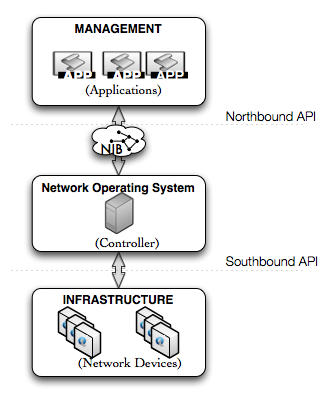
\includegraphics[width=\textwidth]{pic/related/sdn-stack}
  \caption{SDN Architecture}
  \label{fig:related:sdn-stack}
\end{figure}

%The image is misleading in severals ways (for the sake of simplicity). First, the applications (APP) do not necessarily reside outside the control plane. 
%They can be located in memory with the controller process. 
%Second, the network state also does not necessarily reside outside the control plane in a data store. 
%It could also be located in memory, or in extreme do not even exists (e.g., each application maintains its relevant state). 

The network logic operates in the \textbf{Management} plane. 
This plane defines the global network level objectives in the form of one or more (possibly) cooperative applications. 
From a conceptual point of view, these applications interact with the controller through the \emph{North} \gls{api}. 
% In practice this is not always true (explained further along the text). 
A possible implementation of this interface is a \gls{rest}  web service implemented in the controller\footnote{A web \gls{api} based on \gls{http} protocol.}~\cite{fielding2002principled} that allows remote applications to read and modify the network state and configuration.  
It is also possible that controllers allow applications to subscribe (to be process) to network events through this \gls{api}. 
This is typically applicable to in-memory applications but does need to be the case. 
For this reason the image also shows that the controller invokes operations on  the Management plane through the \emph{North} \gls{api}. 
All the control planes referenced in this document allow this behavior for in-memory applications. 
In fact, as we shall see, the event-oriented programming model is present throughout all the \gls{sdn} stack components  being that  \gls{sdn} is event oriented from the get go, as network events  such as  topology changes and forwarding requests, are asynchronous in nature. 

In the \textbf{Control} plane resides the core logic that glues the stack together. 
This component has three major responsibilities. 
First, it is responsible for orchestrating the multiple applications available.
This implies setting up the remote \textbf{North} \gls{api} (e.g., \gls{rest} web server) and maintaining in memory applications that cooperatively manage the network. 
Second, the controller  defines how the \emph{Network State} is shared between  applications. 
In the event that the control plane is distributed, then the controller also defines how the state is shared between controllers. 
%It may also define how this state is shared between controller if the control plane out to be distributed (explained further along in the text). 
%Applications that maintain network state such as topology are commonly provided by  the controller, and usually operate in-memory. 
%usmaintaing a platform where the in memory applications reside that cooperatively builds and maintain the \emph{Network State} with all the relevant information for the control platform in place (e.g., switch and link state,  topology, firewall rules, etc.,).  
Third, it is also in charge of the data plane communication, through the \emph{South} \gls{api}  that enables data plane configuration (e.g., push/pull state from switches). 
Again, the \emph{South}  \gls{api} can be event-oriented whereby events are commonly topology information (i.e., link up, link down) or forwarding requests (e.g., flow tables misses in \gls{of}). 

Finally, the network devices responsible for packet forwarding reside in the  \textbf{Data} plane. 
Any device can be used (wireless access point, Ethernet Switch, router), as long as it implements the \emph{North} \gls{api}\footnote{In practice a mixture of both north enabled  enabled devices and normal devices is possible. Those are known as hybrid networks by the \gls{sdn} community.}.
We commonly refer to these elements as switches regardless  of the functions that they perform in a standard mode (without the intervention of a controller). 

There must be connectivity between the Control and the Data plane.
This connectivity can be  \textbf{in-bound} or \textbf{out-bound}. 
In the in-bound case, the connectivity takes place over the network used for data forwarding while in the out-bound case a different and isolated network is used. 
Connectivity between these two layers require manual configuration of the network devices. 

The \emph{West}/\emph{East}  \gls{api} is  the same and exists only when  distributed control is employed (see Section~\ref{sec:related:distr-contr}). 
Then, the controller uses this \gls{api}  for state distribution and controller-to-controller communication. 
It has two flows of communication for functions performed by the controller on another controller instance (e.g., push state, read state, install rules in another switch, etc.,) or in event-oriented  implementations to receive events from other controllers (e.g., state has changed, new data plane event from a switch). 

Finally, we note that \glsplural{sdn} can operate in two different models. 
In the  \textbf{Reactive} model a switch that does not known how to forward a packet can request the controller to chip in. 
The controller can then take action (e.g., forward, drop, log)  and inform the switch. 
Typically (as shown in Fig.~\ref{fig:related:reactive}) the controller updates the switch with rules for both the packet and subsequent packets that will follow it.  
In contrast, in a \textbf{Proactive} model the switch does not contact the controller with  forwarding requests. 
Instead, the switch is configured according to the management networks objectives. 
Whenever this objectives changes or the network state changes (e.g., link goes down) then the control plane updates the configuration of the switches. 
We note however that the current \gls{sdn} technology is pliable enough to have both models. 
One can even choose between the two models for different types of traffic, or different periods of time in the same \gls{sdn} deployment. 

\subsection{OpenFlow}
\label{sec:related:openflow-spec}
\glsreset{of}
%Missing things to talk about:
% \begin{itemize}
% \item FLOW REMOVED (evaluation section, maybe we can remove it). 
% \item FLOW MOD  (evaluation section, maybe we can remove it). 
%\item it is event-driven, the switch does not need a reply
% \end{itemize}
\gls{of} is the most common implementation of the \emph{South} \gls{api} shown in Fig.~\ref{fig:related:sdn-stack} which consequently has  
somewhat defined the current panorama of \gls{sdn} architectures. 
Thus, in order to make this document self-contained we feel that we should clarify some technical aspects of the \gls{of}  protocol. 
%This section will briefly resume (and simplify) the most important characteristics of the protocol that should be used as reference for the remaining document. We note that the relevance of this protocol has already been covered in section~\ref{sec:related:openflow}.  

\begin{figure}
  \centering
  \includegraphics[width=\textwidth]{pic/related/openflow}
  \caption[Flow Request ]{Commonly, in an reactive model, the first packet of an flow for which there is no match is forwarded to the controller which evaluates it and decides the appropriate action. Normally it modifies the switch flow table such that the packets that follow do not have to go to the controller. }
  \label{fig:related:reactive}
\end{figure}

\begin{table}[ht]
  \centering
  \begin{tabular}[ht]{lll}
    Match Fields &  Instructions & Timeouts \\ \toprule 
    source MAC = 10:20:. \emph{AND}  protocol = ICMP  & port 2,3 & 5,10 ms \\ 
    source IP = 10.0.0.0/24  & port 1 &  0/0 \\
    source IP = 10.0.0.0/24 \emph{AND} protocol = TCP & controller & 0/0 \\ 
    any & controller & 0/0 \\ \bottomrule 
  \end{tabular}
  \caption[Openflow Flow Table]{Simplified representation of a flow table in OpenFlow switches.}
  \label{tab:related:openflow-flows}
\end{table}

Table~\ref{tab:related:openflow-flows} shows a representation of an \gls{of} table present in the switch.
This table is used by the controller to define the forwarding rules for each packet in the network that passes through the switch. 
%The switch uses the match fields to find the forwarding instructions for any incoming packet.
As opposed to common devices, which are restricted to a small set of network packet headers (e.g., \gls{mac} for switches, \gls{ip} for routes), \gls{of} switches are able to match packets against 13 different headers (that can be combined with logical operators).
Furthermore, some headers such as the \gls{ip} and \gls{mac}
 fields can be matched against  bitmasks which allows  a wide range of values for a single table entry. 
As an example, the table shows that the last two entries match against any host present in the $10.0.0.0/24$ network. 
Beyond headers, the switch can also match packets according to the port on which they arrive. 
We note that conflicting matches (i.e., a packet matches more than one entry in the table) are arbitrated by the priority associated with the rule (not show in the table). 

For each entry there is an associated instruction that the switch uses to forward the packet whenever it is able to find a match. 
Several instructions are available including: forward to port $x$, forward to controller, and drop the packet. 
As seen in the table, the instructions can be combined (the first entry forwards to two different ports). 


Each entry  is removed from the table once one of the two private timeouts expire. 
There is an hard timeout, which is never reseted,  and an  idle timeout that is reseted whenever an packet is matched against the entry. 
Both timeouts are used by the controller to recycle and control the entries in the switch table.
It is also possible that a rule is persistent (never expires). 
In this case the timeout will be set to 0. 


A \gls{of} switch table can be configured to forward non-matching packets to the controller (e.g.,  the last entry in the table).
In a  reactive model, the switch forwards the first packet of a flow to the controller. 
In this context flow is somewhat undefined but in essence it should represent a stream of one or more packets in an communication.
For example a flow could be all the packets exchanged between an \gls{http} client and server to download a web page, or it  all the \gls{icmp} packets exchanged between a pair of hosts. 

Fig.~\ref{fig:related:reactive} illustrates how the switch processes packets in the reactive mode. 
The first packet (1) for some ``flow'' (e.g., download of an web page)  reaches the switch but is redirected to the controller since there is no rule that matches it in  the switch table. 
We call this message (from the switch to the controller)  a flow request or \texttt{packet-in}. 
This request must contain (at least) the packet header from packet 1 that will be used by the controller to determine the reply. 
For this reason we usually abuse the language and say that a packet arrives the controller. 
For example, we might say an \gls{ip} packet arrives at the controller to refer to a flow request caused by an \gls{ip} packet. 
Getting back to our example, when the controller receives a flow request, he processes it  and then replies to the switch with instructions to process the packet. 
Additionally, the controller also configures the switch table such that  future packets in the flow are forwarded directly by the switch. 



%%%%%%%%%%%%%%%%%%%%%%%%%%%%%%%%%%%%%%%%%%%%%%%%%%
\glsresetall

\section{Physically Centralized Controllers}
\label{sec:related:phys-centr-contr}
\glsresetall

%%%%%%%%%%%%%%%%%%%%%%%%%%%%%%%%%%%%%%%%%%%%%%%%%%

In this section we present an overview of relevant centralized
controllers. Centralized controllers are, by our definition, control
planes that do not show any explicit support in the deployment of 
different controllers processes over onde or more servers. 
According to our general architecture (see section~\ref{sec:related:sdn-architecture}) the controller has no \emph{East}/\emph{West} \gls{api}. 


\begin{figure}
  \centering
\includegraphics[width=\textwidth]{pic/related/meta-controller-architecture}
  \caption[Controller Architecture]{The common (meta) controller architecture is event-driven. The data plane triggers events (e) that are dispatched by the controller to a pipeline of interested applications. }
\label{fig:related:meta-architecture}
\end{figure}

All the controllers in this section share the architectural composition shown in Fig.~\ref{fig:related:meta-architecture}.
In this architecture, the controller supports multiple applications that run in-memory (i.e., with the controller process) with the goal of processing events  triggered by the data plane (i.e., the switches). 
For each event $e$ (e.g., link up, new switch, flow request) the switch triggers an \gls{of} message to the controller. 
This, in turn, parses  the message to analyze its type and redirects it to the appropriate pipeline. 
A pipeline, is composed of several stages. 
In each stage a different application processes the event and chooses to pass it further along in the pipeline, or to abort the event processing. 
We note also that any (or all) of the applications could interact with the switches at any time. 
Finally we also notice that this architectures  show a tight-bound between the Management and Data plane interfaces (i.e., \emph{North} and \emph{South} \glsplural{api}) since the pipelines are dependant of \gls{of} events. 

This architecture has been concurrently introduced (see section~\ref{sec:related:netw-oper-syst}) by NOX (covered in section~\ref{sec:related:nox}) and Maestro (covered in section~\ref{sec:related:maestro}).  It was also adopted by Beacon (section~\ref{sec:related:beacon})  and later on Floodlight (section~\ref{sec:related:floodlight}). 
We have evaluated and studied all this controllers considering each one as the base for out distributed controller. 
We end up choosing Floodlight for this and we explain why in section~\ref{sec:related:controller-choice}. 

\subsection{NOX}
\label{sec:related:nox}

NOX\footnote{\url{http://www.noxrepo.org/}} was published and publicly released under
the \gls{gpl} in 2008 \cite{Gude:2008jd}. 
It was developed both in C++ and Python and enables a standard interface for the integration of  Management applications 
in the controller. 
Even though one of the main contributions of this paper is the introduction of the \gls{nos}  abstraction (see section~\ref{sec:related:netw-oper-syst}, NOX itself  is tightly bound to the \gls{of} \gls{api}. 

The NOX programming model is event-driven as shown in Fig.~\ref{fig:related:meta-architecture}.
Applications  register in a
priority based pipeline with event handlers associated to either OpenFlow  or application based events. 
The NOX core is equipped with applications that build a host and switch level topology in the network \emph{view}. 

In NOX applications control network objectives and also cooperate to define the current \emph{view} which is an essential component of the controller. 
The \emph{view} can contain the switch-level topology; the location of users, hosts, middleboxes and other network elements; and the services (e.g., \gls{http}) being offered. 

Interestingly, the authors' point out that this choice of granularity for state (the \emph{view}) is adequate for many network applications while changing slowly enough that it can be scalably  maintained. 
They also argue that the network \emph{view} can be distributed with standard replication techniques for resilience. 
In fact the \emph{view} is a set of indexed hash tables with support for local caching. 
In this regard this vision is very similar to ours but has not been effectively developed in their work. 

Initially, NOX was a single threaded application not focused on performance. 
However, from its publishing date several improvements have taken place \cite{Tootoonchian:2012uia,zen-doc-thesis} that have significantly improved NOX performance. 
Under the set of improvements we highlight the natural evolution to a multi-core aware application that statically distributes network requests to different threads. 

In the time of writing, NOX is publicly available but has ramified into two different applications: A C++ based controller available in Linux and a Python based controller (POX) available for several environments.

\subsection{Maestro}
\label{sec:related:maestro}


A network operating system has (at least) two functions: introduce a layer of abstraction between the network and the applications and control the interaction between applications. Maestro is the undergoing work of Zeng Cai covered in \cite{maestro} is focused in the second. In particular Cai recognizes that Management components (i.e., the applications)  do not operate independently and in isolation. Instead, they operate
concurrently but with inter-dependent state. 
With this in mind it leverages parallell computing techniques to enhance the control plane performance. 

Maestro, as NOX, splits the regular pipeline execution such that it can be concurrently executed. As seen in Fig.~\ref{fig:related:meta-architecture} events may
follow different execution paths since singular applications are not interested in every single event. 
Thus, Maestro can manage to execute several applications concurrently. However, in order to
efficiently coordinate the applications access to the shared state Maestro opts to have a more granular state model. 
The author argues that it is
common that applications are interested only in subsets of the network state. 
In order to employ effective concurrent execution Maestro requires that applications specify  what subsets of the state they require as input and what subsets they modify as output. 

The fundamental objective of Maestro is to maximize scalability in a centralized control plane. To do so it attempts to exploit parallelization in the controller server.  Three major design goals shape Maestro: fair distribution of work across cores; minimal overhead introduced by cross-core and cache synchronization and;
minimal memory consumption. In addition, it also
exploits throughput optimization through batching. 
The results published show that Maestro linearly scales the throughput with the number of cores available on the controller. 

Currently Maestro is available under the LGPL 2.1 licence. It ships with usual switching  and routing capabilities \cite{maestro}.


\subsection{Beacon}
\label{sec:related:beacon}


Beacon is an open source controller built in Java, by David Erickson during his academic studies in Stanford University. 
He is, to our knowledge, the only official maintainer of the
application. 

Beacon is also based on the event-driven model shown before. Applications register for
specific type of events and process these  in the order
configured by the user. Any application processing an event chooses to forward the
event further in the pipeline or terminate its execution. It is also
multi-threaded, binding switches to particular threads.
Applications receive data from all threads.

Applications in Beacon are implemented as \emph{bundles}. 
A bundle is the unit of abstraction in the OSGI \cite{osgi} framework - a component and service platform for the Java programming language with dynamic capabilities - allowing features such as \emph{hot-swapping} (i.e., deploy, start and stop modules in run time). 
Beacon provides a central service (the registry) for registration of bundles as services. 
Each bundle implements a service, exports it to the registry and other bundles may consume it. 
Applications events in Beacon take place through the service abstraction: bundles may register in other bundles as listeners to be notified when specific events take place. 

Beacon does not provide any state management service. The network state is decentralized and encapsulated in the bundle abstraction. There are no persistance  mechanisms also. 

\subsection{Floodlight}
\label{sec:related:floodlight}
Floodlight is an open source Apache licensed controller.
 It was initially forked from Beacon and is developed by an open community of developers mainly composed of Big Switch\footnote{A SDN vendor with a commercial distributed controller named Big Controller \cite{:vn}.} employers. 
It is written in Java, but applications can either be implemented in Java, Jython or through the \gls{rest} \gls{api}  available. 

Floodlight follows the common event driven programming model of most  controllers. 
Although Floodlight was originally forked from Beacon, the OSGI support was taken for performance and deployment reasons. 
The overall functionality is based on modules (i.e., applications) that implement services that can be consumed by other modules. 
It is similar to Beacon in this regard, however the module/service functionality is directly provided by Floodlight instead of delegated to a third-party framework as OSGI. 

Floodlight is also multi-threaded. 
It accomplishes this through an asynchronous event based multithreaded library named Netty \cite{netty} that manages Input/Ouput communication with the managed switches. 

\todo{Talk why we choice Floodlight}
% \subsection{Controller Choice}
% \label{sec:related:controller-choice}
% % \begin{table}
% %   \centering
% % \small
% % \begin{tabular}{cccc}
% % Controller & Applications & OpenFlow version  & COOL Features \\\toprule 
% % Maestro & \begin{tabular}{c}Topology Manager \\ Learning Switch \\ Routing\end{tabular}  & 
%Unknown & State Dependency Control\\ \midrule 
% Beacon & \begin{tabular}{c}Learning Switch \\ Hub \\ Device Manager \\ Topology Manager \\ Layer 2 shortest Path Routing \\ ARP and DHCP Proxy\end{tabular} & 1.0 (No plans for others) & Dynamic Components (OSGI) \\ \midrule
% Beacon & \begin{tabular}{c}Topology Manager \\ Forwarding \\ Device Manager \\ Storage \\ Firewall \\ Static Flow Pusher \\ Learning Switch\end{tabular} & 1.0 (1.3 by March 2013) & Active development \\ \bottomrule 
%   \end{tabular}
%   \caption[Comparison of Open Source Controllers]{Comparison between different open source controllers in 2012.}
% \end{table}
%%%%%%%%%%%%%%%%%%%%%%%%%%%%%%%%%%%%%%%%%%%%%%%%%%

\glsresetall
\section{Distributed Controllers}
\label{sec:related:distr-contr}

\subsection{Kandoo}
\label{sec:related:kandoo}

In 2012 Yeganesh~\etal\ presented Kandoo \cite{Yeganeh:2012jm}  --- an hierarchical controller for scalable infrastructures. 
The main contribution comes from the deployment of isolated controllers near the switches that shield a parent  controller from processing all
flow requests triggered by the network. 
It is implemented in a mixture of
C, C++ and Python and is not publicly available. 

In Kandoo --- see Figure  \ref{fig:kandoo-design} --- the control and management plane is replicated in two two levels: in the top level resides the root controller responsible for normal operation; and in the bottom, local controllers that are (ideally) closer to the managed switches (in fact they may even be implemented in the switches itself). 
This design is motivated by the ideia of bringing control functionality towards the data plane. 


The Management plane exists in both levels. 
\emph{Global} applications reside in the top level and operate with the input of the global network state while \emph{Local} applications reside in the bottom level and operate without the global state. 
Each event can be processed by local applications without the root controller collaboration. 
However, if a local application decides that a particular event requires the input of the network state, or modifies this state than the application can redirect the event to the root controller. 
As the bottom plane does not requires access to the network state it remains simple and efficient. 
Additionally, flow request that can be processed by local applications benefit from a lower latency penalty. 


\begin{figure}
  \centering 
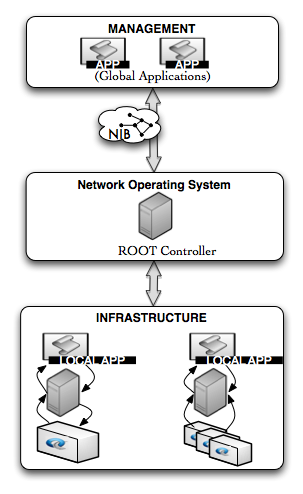
\includegraphics[scale =0.7]{pic/related/kandoo-design}
  \caption[Kandoo design] {Kandoo decomposes the control plane into 
in two levels. The root controller and global applications have access to the global network sate.  The Local controller and applications remain close to the data plane and do not require access to the global state.} 
  \label{fig:kandoo-design}
\end{figure}

%relief 
%The major goal is to shield the root controller from frequent events that could be processed without much knowledge of the network state.
%This two level design allows  shielding the controller from frequent events triggered by the network devices. 


%In Kandoo scalability is supported by the introduction of the two level hierarchy. 
%The bottom control plane  shields the root control from processing of events. 

We conclude with two points. 
First, the Kandoo architecture is complementary to others (even ours). 
%In fact the authors' stress that other distributed control planes and Kandoo can co-exist together. 
Second, Kandoo can effectively scale the control plane further at least in theory. 
However, Kandoo architecture is only as effective as the number of flows that it can process locally. 
%the effectiveness of scalability mechanism depends on a significant number of applications that are able to process flow requests locally without the root controller intervention. 
Unfortunely, the paper does not specifies how practical or significant are  the class of applications that can operate without global state as to process events locally. 

\subsection{HyperFlow}
\label{sec:related:hyperflow}



Motivated by the lack of scalability in centralized controllers, HyperFlow \cite{Tootoonchian:2010vy}  was created as a distributed controller. 
The  authors' aim was to provide scalability without sacrificing the simplicity of management applications  in centralized controllers. 
It is built as a \emph{C++} application on top of the NOX  controller \cite{Gude:2008jd} requiring minor modifications to the controller core and is not publicly available. 

Fig.~\ref{fig:hyperflow-design} shows the overall architecture of HyperFlow. 
The control plane is distributed over different controller instances (or replicas). 
Each instance maintains, under its administrative domain, the connection to a subset of the data plane. In case of failure, there should exist mechanisms that allow other controller to assume control of the failed controller data plane set. 

%Two main components compose this architecture: the controller application (HyperFlow) and an Publish/Subscribe middleware.  
%The controller component is an application, built in NOX, which interposes between NOX applications and the data plane to intercept all communication between the two. 
%To clarify, the controller intercepts event triggered by the data plane or applications as well as the configurations messages sent from the applications to the switches. 
%The controller component is an application built in NOX which intercepts events triggered by the data plane or the applications as well as the   configuration messages sent from the applications to the switches (i.e., commands). 
%In essence the controller interposes between NOX applications and the data plane capturing all communication between the two. 

In HyperFlow, each controller instance is a replica of the entire network state. 
To do so, HyperFlow intercepts any event that has caused changes to the network state (when processed by an application). 
Then, it distributes this event to other controllers that  will also process it. 
This way  --- and assuming that all controller instances run the same set of deterministic application --- all controllers instances eventually arrive at the same state.\footnote{Considering that there are no updates for a sufficient amount of time.}

The positive side in having a view of the entire network is that each controller can take decisions based on the state present locally.
%This state is eventually consistent since it will, at some point in time, be equal in all replicas\footnote{Considering that there are no updates for a sufficient amount of time.}. 
However, the controller still has to communicate with others to distribute state changing events and configuration directives to switches that are controlled by other instances. 


The inter-controller communication system is based on the well-known \emph{Publish/Subscribe} model, whereby one defines publishers as senders of messages and subscribers as the receivers. 
Publishers do not send messages directly  to receivers.  
Instead, messages are published in a medium, and interested receivers selectively receive them through some form of subscription logic (e.g., channel, topics, etc.). 
This model allows the decoupling of both space and time in the communication between publishers and subscribers. 

HyperFlow, leverages on an existing Publish/Subscribe system that provides: persistent storage of the events published; \emph{FIFO}
(First-In-First-Out)  ordered delivery of the messages published by the same controller; and resilience against network partitioning.
%The event propagation system allows  communication between HyperFlow instances and  is built over a distributed filesystem. 
%Communication is done through channels implemented as files. 
%There are three types of channels: the control channel where controllers advertise themselves; the data channel where general interest events are published by every controller;  and finally the individual controller channel for OpenFlow commands relevant to the controller who owns the channel. 

% State distribution in HyperFlow is accomplished through the
% Publish/Subscribe event propagation system. The NIB  is
% replicated in all instances and HyperFlow distributes the events
% that cause changes to it. This is done through event publishing in the shared
% data channel. Every controller subscribes to the
% data channel and replays the events received on it, thus changing its
% NIB in a similar way.  The view  is maintained by the Management applications
% residing in the controller and outside the domain of
% HyperFlow (as in NOX). HyperFlow is, in concept,  identical to a \gls{smr} system with the controllers as replicas. State changing events are distributed to all replicas, that execute them to converge to the same state of others. 


%Additionally, Hyperflow  also addresses incorrectness problems caused by transient inconsistency across controllers  by defining an \emph{authoritative}  controller for each flow. This controller is responsible for orchestrating changes in the network regarding some flow. As an example, to avoid loop-free forwarding \emph{authoritative} controllers are solely  responsible for setting the flow paths across the forwarding plane for some specific flow. For this, applications must relay requests for some flow to its \emph{authoritative} controller. 

HyperFlow addresses scalability of the control plane by minimizing the number of events that an instance replicates to others. 
Thus, HyperFlows s focus on the scalability of the CPU and does not address state scalability since  each controller contains  the entire network state. 

To minimize the number of events  processed by instances, HyperFlow filters the dissemination of events.  
To this end, it requires that applications tag locally generated events that affect the network state.   
Only these events are worth distributing,  as others are redundant. 


%Local events are generated either by the management or data plane layers but applications trigger events as a response to the processing of other events (i.e., there is a causality relationship between events). 
HyperFlow minimizes distribution of events even further by tracking events that cause other events. 
For this reason applications triggering events have to  associate the event that caused it. 
If, for example, some event $e_2$ is triggered due to the processing event $e_1$, it  distributes only event $e_1$. 
This is enough since the applications are equal in all controllers. 
Thus,  the processing of $e_1$ will  trigger event $e_2$ in all replicas. 
As one single event can cause several application events to be triggered this can reduce the volume of traffic and processing of redundant events.

\begin{figure}
  \centering 
  \footnotesize
  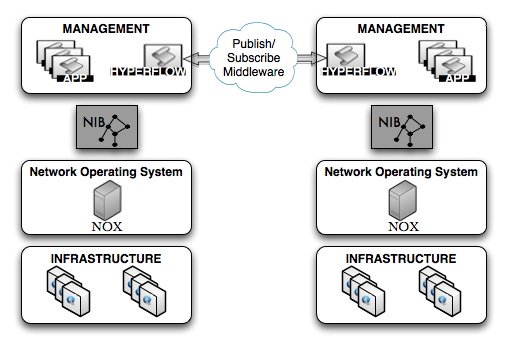
\includegraphics[width=\textwidth]{pic/related/hyperflow-design}
  \caption[HyperFlow architecture]{HyperFlow architecture. The two major components are the controller which intercepts events and configuration commands that must be distributed and the Publish/Subscribe system used for all communication between controllers.} 
  \label{fig:hyperflow-design}
\end{figure}

%Applications running on HyperFlow act as they control the entire network.
%Behind the scenes, HyperFlow redirects requests to the network equipment  to the controller equipment which the request addresses. 
%HyperFlow also routes back  responses to the controller responsible for  the request. 

One of the advantages of HyperFlow is that the existent applications are barely modified in order to work in a distributed control plane. 
Furthermore, the programming model itself is identical to NOX  (event driven, pipeline based) which maintains its simplicity and quite transparent since applications behave as they were running the all network. 
%Some overhead complexity is added as HyperFlow requires the applications to tag  state changing events and identify parent events as explained above. 

However, this is not quite true since applications do have to account for the restrictions of the underlying distribution system. 
For example, applications are limited to change state based only in events that arrive from a single switch. 
A complex Load balancer that wishes to perform aggregation calculations on more that one link across different switches would possibly result in divergent state across controller replicas. 
Notice that even with FIFO based channels some controller $c$ might receive event $e_i$ followed by event $e_j$ sent from controllers $i$ and $j$, while a controller $c'$ perceives $e_j$ followed by $e_i$. 
Thus, It is possible that such occurrence leads controllers to divergent states if applications modify state relying in event ordering across different entities. 
%For this not to happen each switch associated state could as well be completely isolated from
%The article explicitly adverts that Management applications should not rely in event ordering "except those targeting the same entity (e.g., the same switch or link)'' as those guarantee FIFO ordering. 

Another benefit of HyperFlow is that under read intensive workloads the controller can achieve low response times since  events are processed locally.
However in our experience with centralized applications (as the ones that HyperFlow targets) read intensive workloads are not too common.
In fact, Chapter~\ref{sec:feasibility:apps} shows that  three (out of three) applications in the Floodlight controller show at least one write operation for each event processed at the controller. 
We note that those applications are fundamental for tracking hosts, forwarding and round-robin load balancing and they could not easily  avoid that write operation without incurring in non-optimal behavior (i.e., they would be less correct in the goal they promise to achieve). 

%Finally, while HyperFlow is robust in the face of failure it does so at the expense of the controller resources. 
%Under failure it has to replay all events. This can be time consuming and events grow indefinitely. Under this time the controller can not serve requests. If instead this recovery mechanism is isolated from the controllers then a recovered controller (or other in its place) can start processing network events almost immediately. 
%Another benefit it that it requires minor modifications to a centralized controller. We note that this not exactly true. Given the restrictions imposed by the \gls{fifo} semantics of the publish subscribe middleware, the applications are not able to rely not even on causality modifications to the network state. An Load Balancer application that typically relies on different switch state to manipulate 


\subsection{Onix}
\label{sec:related:onix}

Onix \cite{Koponen:2010th}  was build upon the NOX legacy and provides two major contributions: it is the first general controller published in the literature, and also the first to provide strong consistency.  
Onix  provides an improved Network Operating System interface on  which the northbound API does not reflect the southbound API. 
Management applications are programmed against a network graph of Typed Entities very similar to the Object Oriented paradigm and are not aware of the southbound characteristics (e.g., the use of \gls{of}). 
The graph is implemented in  the \gls{nib}  --- a in-memory data structure that contains the network state ---  and can be distributed across a  cluster of  Onix controllers. 
Applications have the choice to specify consistency and durability requirements  per network entity  present in the \gls{nib}.  
Onix was the result of a joint effort between Google, NEC, Nicira, ISCI and Berkely, and (at least)  both Google and Ericson have developed their controllers based on from Onix \cite{The-Valley-of-the-Nerd.:fk}. 
At the time of writing Onix is not publicly available. 

Onix architecture is presented in figure \ref{fig:onix-design}. 
Only one application resides on the  Management layer and may communicate with other applications in other controllers instances for coordination. 
The \gls{nib} is the only element in Onix northbound interface. 
The Management layer directly modifies the \gls{nib} and subscribes to changes on it. 
The data plane  indirectly modifies the \gls{nib} (trough the controller).


The controller  has to guarantee that changes in the Infrastructure are reflected in the \gls{nib} and vice versa. 
For this, it translates network events into changes in the \gls{nib} and changes in the \gls{nib} to changes in the data plane configuration. 
Onix supports  \gls{of} but it could transparently move to another southbound API. 

Each Onix instance independently manages a subset of the data plane. 
However each instance can be exposed to the entire network state through  the \gls{nib}.  
Under such scenario, each time a local Onix instance alters the \gls{nib}, these changes are reflected in all other instances. 
Thus, the \gls{nib} is also the distribution mechanism of the Onix controller. 
The distribution itself is done by the datastores that back up  the \gls{nib} state (seen in figure \ref{fig:onix-design}).
However, in concept the \gls{nib} is not meant to contain all the network state. 
In fact, the \gls{nib} is best seen as a kind of in-memory cache which imports (exports) particular state from  (to) the fault-tolerant distributed data stores. 

\begin{figure}
  \centering 
  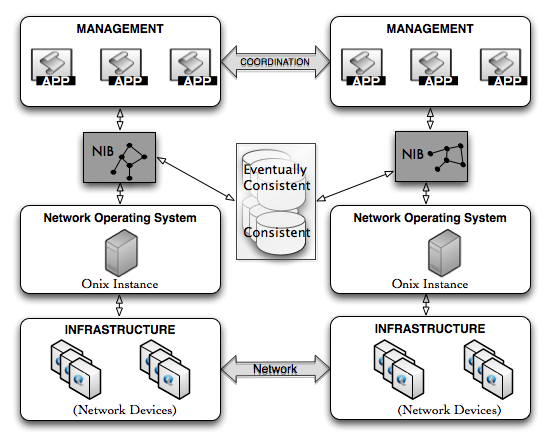
\includegraphics[width=\textwidth]{pic/related/onix-design}
  \caption[Onix architecture] {\textbf{Onix achitecture.} In Onix the NIB is the
    solely entity used as the northbound api and Managements program
    directly against it. The NIB is supported by
    two replicated datastores accessible across Onix instances.  The
    Management layer communicates across instances for coordination.}
  \label{fig:onix-design}
\end{figure}

% \begin{figure}
%   \centering 
%   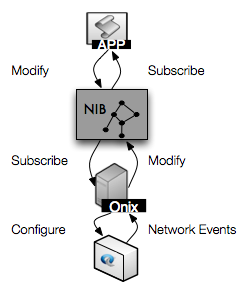
\includegraphics[scale=0.5]{pic/onix-process.png}
%   \caption[Onix configuration process]{\textbf{Onix configuration
%       process}. The interactions between layers of the Onix
%     instance stack. In the figure we can observe the process of
%     configuration on the left side, and the process of detecting
%     changes in the Infrastructure on the right side.\footnote{The Infrastructure should be only one.}} 
%   \label{fig:onix-process}
% \end{figure}

Onix defines a flexible distribution model for the \gls{nib} whereby  it offers the application designer the choice of consistency guarantees. 
Two replicated data stores are present, covering  strong  and eventually consistency. 
Strong consistency data is provided through a transactional persistent database backed up by a replicated state machine (see section~\ref{sec:related:cons-data-stor}). 
This data store is favored for data with low-frequency changes  as its performance limitations are significant. 
The eventually consistent data store consists in  an one hop memory based \gls{dht}  (as Dynamo  \cite{DeCandia:2007cn}) favored for  volatile data with high update rates. 
%The \gls{nib} reflects the state of both data stores. 
Both the integration of multiple data stores and the inconsistency characteristics of the \gls{dht} can lead the \gls{nib} to an inconsistent state where reads performed in some entity may return more than one result. 
Thus, Onix provides primitives for the integration of inconsistency resolution logic as well as  direct integration of a distributed coordination framework (see  Apache' ZooKeeper \cite{Hunt:2010ux}) in the northbound interface. 

Onix is intended for large scale network infrastructure where scalability is fundamental. 
However, in each Onix instance the \gls{nib}  size reflecting the network state could lead to memory exhaustion and the processing of both network events and subscriptions  to changes in  the \gls{nib}  can lead to \gls{cpu} exhaustion.
In order to introduce scalability and avoid exhaustion, partition and aggregation based techniques can be configured in the Management layer. 
Partition avoids full replication of both data  and workload such that additional instances do not only replicate overall work but also relief it. 
As for aggregation it can, for example, allow network entities to be aggregated and exposed for other Onix instances as only one.
In practice partition in Onix is present in the division of the data plane across different Onix instances.  
This way instances process fewer events. 
Additionally the Management logic can configure Onix instances to keep only subsets of the \gls{nib} in memory and up to date. 
For aggregation, an Onix instance can be configured to expose a subset of the \gls{nib} as an aggregated element. 
%MISSING THINGS . To exemplify a controller could export, to the data stores, its network topology as a single 

Applications are built against the \gls{nib} graph data structure that is composed of \emph{Typed Entities} supporting the Object Oriented paradigm (i.e., encapsulation of data, functions over entities, hierarchy, etc.). 
Onix supports extensible representations of network entities. 
The \gls{api}  provides essential functions to search, inspect, create, destroy and modify entities present in the \gls{nib}. 
It is also possible to register notifications for creation, removal and updates of data entities. 
When network events of other Onix instances update the data stores those changes must be reflected on the local \gls{nib} and the application must be notified through a callback function. 
All operations are asynchronous, with eventual delivery and no ordering or latency guarantees given therefore a \emph{barrier} synchronization primitive is available allowing the application to wait as updates are translated and applied in the network devices and/or other controllers. 
Finally it is worth mentioning that Onix employs coarse-grained locking mechanisms over the \gls{nib}.
 Applications are given the guarantee that no other local thread concurrently updates the \gls{nib}. 


Onix is focused in generality; and it does a great job at it. 
However it is merely an control platform where the Management application has to fill-in to complete  most of the work. 
Namely, neither reliability nor scalability are first class citizens of the platform. 
Furthermore, beyond delegating reliability for the developer, Onix relies on third party applications for this task (i.e., Apache' Zookeeper~\cite{Hun10} ). 
This, it introduces another degree of complexity for the \gls{sdn} developer which has to learn yet another interface. 
As a contrast, in our controller design the same interface is able to perform all the tasks which (arguably) presents a less steeper learning curve.  

It is important to realize that Onix is in no way optimized for performance. 
As stated in the paper: ``when faced with a tradeoff between generality and control plane performance we try to optimize the former while satisfying the latter''. 
This is fine, but it lefts us (the world) with a gap in the research field. 
Namely we need to understand what kind of impact does a reliable and distributed control plane has on real world \gls{sdn} applications. 
Furthermore, we need to effectively contrast eventual consistency vs. strong consistency distributed control planes. 
To clarify, not even the Onix eventual consistent  data store evaluation is able to show a significant performance advantage against an off-the-shelf consistent data store.  
This is bad, since enterprises currently, have no way to accurately determine, based on the number of events generated by their data planes, what kind of consistency semantics they should seek for their distributed \gls{sdn} deployment. 

Finally we note that Onix is all but transparent. 
Applications have to include conflict resolution logic, and rely on different interfaces for the appropriate semantic per action. 
To clarify, applications must choose between eventual consistency, strong consistency, à priori in a statically defined import/export module. 
Furthermore, they must rely on complex event oriented programming techniques and specific \gls{nib} methods as the barrier primitive or external interfaces as Apache Zookeeper to modify state with a coherent and reliable semantics. 

%%%%%%%%%%%%%%%%%%%%%%%%%%%%%%%%%%%%%%%%%%%%%%%%%%
\glsresetall
\section{Consistent Data Stores}
\label{sec:related:cons-data-stor}

The key idea of our controller architecture is to make the controller instances coordinate their actions through a dependable data store in which all relevant state of the network and of its control applications is maintained in a consistent way.
This data store is implemented with a set of servers (replicas) to avoid any single point of failure, without impairing consistency.
One of the most popular techniques for implementing such replicated data store is \gls{smr}~\cite{Schneider:1990vy,Lam98}.

The  \gls{smr} technique provides one of the most strongest consistency model known in distributed systems named linearizability. 
This model is completely transparent for the client of the system; so transparent that it is indistinguishable from a centralized (i.e., non-replicated) system. 
Off course, this is at the expense of performance, and more importantly availability since in order to operate it requires a majority of the systems replicas to be accessible. 
The remaining spectrum of consistency models is under the umbrella of the eventual consistency semantics. 
%This model is somewhat undefined, and can support quite mean different  
With eventual consistent data stores, data is also replicated in different replicas. 
However, several problems can emerge from this model including (but not limited) the loss of updates and  conflicting values. 
We give a detailed description and examples of both consistency models in section~\ref{sec:related:underst-cons}.

Practical crash fault-tolerant replicated state machines are usually based on the Paxos agreement algorithm for ensuring that all updates to the data store are applied in the same order in all replicas (thus ensuring consistency)~\cite{Lam98}. 

However, since the original Paxos describes only an algorithmic framework for maintaining synchronized replicas with minimal assumptions, we instead describe --- in section~\ref{sec:related:viewst-repl} ---- the Viewstamped Replication (VR) protocol, a similar (but more concrete) state machine replication algorithm introduced at the same time~\cite{,Liskov:2012ut}\footnote{Also, the Paxos algorithm is known for being hard to understand.}.


State Machine Replication is a fundamental technique that is used by real world systems in a wide array of applications. Furthermore, and contrary to popular believe, it can be used in systems where  availability and performance are crucial requirements.  As so, in section~\ref{sec:related:state-mach-repl} we give an overview of state of the art performance of \gls{smr} based systems. 


\subsection{Eventual Consistency}
\label{sec:related:underst-cons}

To understand consistency we must first establish some fundamental concepts. 
In our context the consistency discussion and tradeoffs arises from data replication systems such as data stores. 
Those systems are replicated for reliability and/or performance. 
The reliability benefit arises from the fact that failures are often the rule and not the exception. Therefore, data must be replicated across different servers in order to survive the time challenge. 
As for the performance benefit in can be manifested in two different forms. First, different replicas can be located closer to different clients therefore improving on the latency. Second, client load can be balanced across different replicas therefore improving the limit on the system processing rate. 


Since the proof of the CAP theorem in 2002 by Gilbert and Lynch that there is an significant  interest in weak consistent distributed systems~\cite{Gilbert:2002il}. 
This theorem establishes that a distributed system can only be qualified with only two of the following properties: consistency, availability and partition-tolerance. 
In this context, consistency is equivalent to a system supporting linearizability (which will be defined in a moment), availability is equivalent to the guarantee than any request performed on the system eventually receives an reply, and partition-tolerance implies  tolerating arbitrary message loss. 
Being that systems  often exhibit arbitrary message loss caused by the network or other pitfalls (the nodes might be  stuck processing the garbage collector algorithm) systems are force to choose between availability and consistency. 

Facing those facts a replicated system is either consistent or eventually consistent. 
If consistent than it is not always available; if eventually consistent it is always available. 
But in practice systems are not black or white. 
In fact, one of the outcomes of the dichotomy established by CAP is a panoply of systems with different consistency models that attempt to position themselves at a different optimal point between  the availability and consistency spectrum. 
To explain, if we look under the hood of eventually consistent, we will conclude that  this model is an umbrella for different consistency models that can be ``more or less'' consistent (e.g., read-your-writes, causal consistency, session consistency). 
Due to space constraints we cannot cover each of those models and instead defer the interested reader for surveys on the topic \cite{bailis2013eventual, bailis2013eventual}

%For simplicity we will focus on the contrast between eventual and strong consistency. 

%To simplify the discussion let us imagine that each client can only issue a single write operation. 


Under the \textbf{eventual consistency} model when a write is finished, then the model promises that at some point in time all clients will converge to the same value. 
The benefit with those models is that they are straightfoward to implement. 
A replica can accept client requests, process them, return the result and only later spread the outcome to others. 
The process of spreading values to others is commonly known as anti-entropy and can take several forms but it in essence an asynchronous (i.e., after replying to the client) process. 
Therefore, several ``bad'' outcomes can come out of it. 
We will show three. 

For support, let us imagine a replicated system with three replicas and only a single register containing some arbitrary value. There are two clients of the system: client 1 and 2 that can perform write and read operations on this register. Fig.~\ref{fig:related:eventual} shows the system composition with two examples of different client requests orderings. 

\begin{figure}
  \centering
  \begin{subfigure}[b]{0.5\textwidth}
                \centering
                \includegraphics[width=\textwidth]{pic/related/eventual-conflict}
                \caption{Stale data: reading an old value.}
                \label{fig:related:eventual-stale}
        \end{subfigure}%
        ~
        \begin{subfigure}[b]{0.5\textwidth}
                \centering
                \includegraphics[width=\textwidth]{pic/related/eventual-stale}
                \caption{Conflicting data.}
                \label{fig:related:eventual-conflict}
        \end{subfigure}
  \caption[Eventual Consistency pitfalls]{Two clients of a replicated data store experiencing some of the eventual consistency model pitfalls. In the stale data case Client 2 is not able to see the last write done to the data store. As for the conflicting data case the concurrent update done  by two clients causes the data store to become confused as to what value it should keep.}
\label{fig:related:eventual}
\end{figure}


First,  Fig.~\ref{fig:related:eventual-stale} shows than while replicas have not converge on client updates other clients are able to see older values of the register. 
Namely, client 1 performs an update on the data store ($write(x)$) and after an certain amout time client 2 stills sees the older value of the register ($Y$). 
We note that with weak eventual consistency models not even Client 1 could be assured to read X in a follow up operation. 
This particular safety property is known as read-your-writes consistency and commonly requires that clients contact with the same replica of the system\footnote{Off course this is only the case for eventually consistency systems. Strong consistency does not imposes this restrictions abeit offering read-your-writes guarantee.}. 
The time period between a write being applied in a data store replica and all clients being able to see that value is named the \textbf{window of inconsistency}.  A position paper on eventually consistent systems states that this window of inconsistency is bound between 200 ms to 15 seconds in different types of systems\cite{bailis2013eventual}. Due to the differences in the environment where those tests were performed we show those values as reference to show that state of the art eventually consistent data stores maintain a lower bound of 200 ms. 

It might be the case that the bound on the  window of inconsistency is not problematic for the users of the  data store. 
However a subtle problem can emerge from the asynhronous anti-entropy process ---- there is no guarantee that an update will reach other clients. 
This it to say that when gets a reply from a server to an update operation (e.g., $write(x)$)  he can not be sure that this update will eventually be seen at other clients. 
First, it might be the case that concurrent updates from other clients cause the loss of the update. 
Surely this is also the case for consistent data stores, but it also true that it is much harder to contradict this behaviour in eventual consistent systems than in strong consistent systems (to see an example of this see section~\ref{sec:heimdall:versioning}). 
Second, and arguably more serious problem than the one identified in the previous argument, it might be case that the server that processed the update fails before spreading it to other replicas. 
In the event that this happens, it can also be the case that recovery is not supported by the system which ineviatably leads to updates being lost forever. 
Thefore, eventually consistency ensures convergence only if replicas survive long enough do spread updates to others. 


Finally, in the event of concurrent updates to a particular data bucket (e.g., our register) eventually consistent systems are forced to deal with conflicting values. 
Fig.~\ref{fig:related:eventual-conflict} exemplifies that  both clients concurrently update the register. 
Then, imagine that two different data store replicas (out of three) process and reply to the clients independently. 
Later on, the anti-entropy process takes place. The question that must be answered then is the following: how out the replicas be able to determine which update should persist between the two ($write(X), write(Y)$). 
Surely only one can be choosen, and undoubtely in many cases it should be lastest. 
However without heavy-weight premises and abstractions  such as the ones used in real-time systems it becomes impossible to determine which update was the lastest. 
Furthermore, it might be the case that the client 1 write is more important than client 2. 
Eventually consistent systems diverge in how they arbiter conflicts. 
Commonly either the system solves the conflict automatically without user intervection, or both values are kept and the uses out to solve this. 
Given that from the system point of view data is just an opaque arbitrary collection of bytes (i.e., raw data) , it is forced to crude arbitration such ``last-write-wins'' (which is commonly not based on a global wall-clock time). It is also the case that more sophisticated systems have a more deep understanding of their data. 
For example, the use of a \gls{crdt} such as a set allows the data store to follow a simple conflict resolution policy  based on a simple union of all the conflicting sets~\cite{shapiro:inria-00555588}. 
On the other hand, delegating conflict resolution to the clients leverages the benefit that the latter is well-aware of the data schema present in the data store as well as the semantical meaning of the two conflicting values. 
As such it can be better equipped to choose how to solve conflicting values.
Notwithstanding  the evidence that systems are equipped to deal with conflicts they do so at the expense of possible incorrectness (in the system case) or the extra effort required from the developer that has to anticipate conflict resolution code for different types of data. 

%Two different approaches can be taken: the system can choose one of the conflicting values and discard all the others; the system can keep both and the 
%In contrast, with the strong consistency model users are not able to discover that data is replicated. 
%In fact the client of systems that provide this model are not able to distinguish him in any way from a centralized system. 

In general, eventually consistent data stores are better equipped to deal with volatile data that does not have stringent requirements such as consistency and reliability.
With the lack of consistency clients are not able to reliable  synchronize with others nor can anticipate the results of an update. 
To combat this lack of guarantees clients must develop counter-measures when dealing with more sensible data that can not rely on the pitfalls seen in this section. 
This implies that additional effort and time must be taken from developers being that in the end they are still subjected to corner cases that they were not able to anticipate  that could arguably result in the failure of the overall system. 

%In opposition the use of strong consistency 
%The users of an eventual consistency are not CONDENADOS to all this pitfalls. However as stated by Bailis et. al, the user has to ``compensate'' for the lack of consistency.  There are techniques that avoid this A \gls{crdt} CRDt's Although these are prominent research topics, these are still concepts difficult to master to the regular developers.

\subsection{Strong Consistency}
As Fekete and Ramamrithan so eloquently state : ``the principal goal of research on consistency models is to help application developers understand the behavior they will see when they interact with a replicated storage system, and especially so they can choose application logic that will unction sensibly''. \cite{fekete2010consistency}
Indeed, for the user a properly defined semantics associated with the requests performed on replicated systems is of paramount important. 
Without it, the user might be able to commit ``mistakes'' that sacrifice the reliability of the data. 
In this context, the most significant advantage of the strong consistency model  is that developers can relax their concern towards the semantics of the replicated system being that a strong consistent system is not any different from a centralized (single site), unreplicated system --- there is no more transparent system that this. 

Truly, the strong consistency property is formally introduced as linearizability~\cite{herlihy1990linearizability} in a seminal paper by Herlihy~\etal. 
In the paper the reader may find a formal definition of linearizability. 
Informally, this property establishes that every operation performed on the replicated systems appears to have effect instantaneously. 
The practical consequence is that clients can be made sure that after receiving a reply from the system for an update operation every other client will be able to see the effect of that write. In practice, this condition is true as soon as the data store processes the client update, but it makes more sense, from the client point of view, to base this assumption only as soon as the reply arrives since it has no other mean to determine that the data store has processed his operation. Fig.~\ref{fig:related:strong} exemplifies this condition. 

Strong consistency is great, since clients are now able to accurate rely on the data store reliability property as soon as they receive a reply. 
To exemplify, the \gls{smr} technique that we use (covered in the following section) blocks client requests until they are processed by a majority of replicas that compose the system. 
Given that this techniques assumes that there will always be a majority of replicas ``alive'' (i.e., non faulty) and reachable, the client is made sure that the aforementioned operation will never be lost in the data store unless it is overwritten. 
However, using simple concurrency control techniques (see section~\ref{sec:heimdall:versioning}) clients can also be sure that no client will innocently overwrite its data without at least  be made aware of it. 
If clients behave correctly they can always confirm in the data store that they are aware of the least-recently-update thus avoiding overwriting data.

\begin{figure}
  \centering
  \includegraphics[width=0.5\textwidth]{pic/related/strong-consistency}
  \caption[Strong Consistency Semantics]{Strong Consistency Semantics. A client can be sure that every client see its operation outcome as soon as the data store replies.}
  \label{fig:related:strong}
\end{figure}
Strong consistent or linearizable distributed systems enable coordination between distributed applications. 
Coordination is a complex problem. For this reason it is desirable to solve once in a generic fashion such that different applications can make benefit from its application. 
A common example of coordination use cases is group membership and leader election.
It is often the case than distributed nodes need to known which nodes are alive and partition responsibility amongst them. 
There are several applications inspired by those particular problems such as Apache' Zookeeper~\cite{Hun10} and Chubby~\cite{burrows2006chubby}. 
And at the very heart of it relies protocols that guarantee strong consistency in distributed replicated systems. 

\subsection{ViewStamped Replication}
\label{sec:related:viewst-repl}
\glsreset{smr} 
The Viewstamped (VR) protocol provides a transparent \gls{smr}  behavior that can be leveraged to implement a replicated data store with strong consistency semantics~\cite{Liskov:2012ut,Liskov:2010vt}. 
The algorithm is built over  an partial-asynchronous network model with a crash-recover failure model for the participants (\emph{replicas}) who are the basis for maintaining a data service  available to clients. 

\gls{smr} allows a set of machines to provide a replicated service, usually to support  availability and reliability characteristics in the system~\cite{Schneider:1990vy}.  
Informally,  the model states that a distinguished set of machines who start in the same state and execute the same set of instructions in the same order achieve the same state  and generate the same output. 
\gls{smr} is suitable for  distributed applications, such as  file systems or lock managers which can  be built on top of the distributed state machine. 

The failure and timing model establishes that replicas may stop (due to crash), perform computations arbitrarily slow or  be isolated from the rest of the group. 
The remanning  group detects and suspects the replica has failed as a reaction to its lack of feedback.
VR allows replicas to re-join the group as long as they are updated on the missed executions by the other replicas.
VR  runs in a Replica Group composed of at least $2f+1$ replicas and assumes that only $f$ replicas can fail simultaneously. 
Thus, as long as $f+1$ replicas are accessible the protocol guarantees liveness (which translates to availability from the client point of view). 

\begin{figure}
\centering
\includegraphics[width=\textwidth]{pic/related/vr.pdf}
\caption[Paxos/VR update protocol]{Paxos/VR update protocol.} 
\label{fig:paxos} 
\end{figure}

VR is based on  \emph{total-order}, a ordered delivery guarantee between a set of machines communicating in group. 
The protocol has a behavior structured around the notion of a leader (a distinguished replica named primary) who chooses and imposes the order of delivery of executions on the group. 
This approach has the drawback of overloading the primary with client requests but  simplifies the protocol and reduces execution latency significantly. 


Fig. \ref{fig:paxos} shows the messages exchanged in VR for an update operation: the client sends a message to a primary replica (the leader) that disseminates the update to all other replicas. 
These replicas write the update to their log and send an \texttt{ACK} message to the primary.
In the final step the leader executes the request and sends the reply to the client.
If the primary fails, messages will not be ordered and thus a new primary will be elected to ensure the algorithm makes progress.
When read-only operations are invoked, the leader can answer them without contacting the other replicas.
Strong consistency is ensured due to the fact that all requests are serialized by the leader.

Off course this is only the normal execution of the protocol. 
The interest reader is forwarded to the originals papers  for a description of the remaining protocol which involves a protocol for re-electing a new leader of the system whenever the current is suspected to fail and also a protocol for recovering replicas such that they can be updated by the group~\cite{Liskov:2012ut,Liskov:2010vt}. 
%Each replica runs the same application code as each can be the primary at some point in time.



\subsection{State Machine Replication Performance}
\label{sec:related:state-mach-repl}
The Paxos/VR algorithm has served as the foundation for many recent replicated (consistent and fault-tolerant) data stores, from main-memory databases with the purpose of implementing coordination and configuration management (e.g., Apache'  Zookeeper~\cite{Hun10}), to experimental block-based data stores or virtual discs~\cite{Rao11,Bol11,Bes13}, and even to wide-area replication systems, such as Google Spanner~\cite{Corbett:2012uz}.
Besides the synchronization protocol, these systems employ many implementation techniques to efficiently use the network and storage media.

Although not as scalable as a weakly consistent data store, these systems grant the advantages of consistency for a large number of applications, namely those with moderate performance and scalability requirements. To give an idea of the performance of these systems, Table \ref{table:smr-results} shows the reported throughput for read and write operations of several state-of-the-art consistent data stores.

\begin{table}
  \center
    \begin{tabular}{ lccc}
    \hline
    \emph{System} & \emph{Block Size} & \emph{kRead/s} & \emph{kWrite/s} \\ \toprule
    Spanner \cite{Corbett:2012uz} & 4kB & 11 & 4 \\ 
    Spinnaker \cite{Rao11} & 4kB & 45+ & 4 \\  
    SCKV-Store \cite{Bes13} & 4kB & N/R & 4.7 \\ 
    Zookeeper \cite{Hun10} & 1kB & 87 & 21 \\ \bottomrule 
    \end{tabular}
  \caption[Performance of state machine replication systems]{Throughput (in thousands data block reads and writes per second) of consistent and fault-tolerant data stores based on state machine replication (N/R = Not Reported).}
  \label{table:smr-results}
\end{table}

Given the differences in the design and the environments where these measurements were taken, we present these values here only as supporting arguments for the possibility of using consistent data stores for storing the relevant state of SDN control applications.
Depending on the specific application this state may include, for instance, a subset of the Network Information Base (NIB).
Interestingly, these values are of the same order of magnitude of the reported values for \emph{non-consistent} updates in Onix (33k small updates per second considering 3 nodes~\cite{Koponen:2010th}), and much higher than the reported values for their consistent data store (50 updates/second for transactions with a single update).
The Onix paper does not describe how its consistent database is implemented but, as shown by these results, its performance is far from what is being reported in the current literature.

%%%%%%%%%%%%%%%%%%%%%%%%%%%%%%%%%%%%%%%%%%%%%%%%%%
\glsresetall
\section{Consistent Data Planes}
\label{sec:related:consistent-data-plane}


\subsection{Consistent Updates}
The authors' recognize that networks are in constant change. 
Routing policy, access control for severals reasons. 
Updates can disrupt the network. 

%%% Local Variables: 
%%% mode: latex
%%% TeX-master: "../PEI"
%%% End: 


\LIMPA
\begingroup
\renewcommand{\cleardoublepage}{}
\renewcommand{\clearpage}{}
\chapter{Architecture}\label{chapter:3}
\endgroup
\epigraph{\emph{All problems in computer science can be solved by another level of indirection...except for the problem of too many layers of indirection.}}{Kevlin Henney's}
%\epigraph{Estamos no Mato...  E sem cão!}{Professor de LEI - 3º ano}
\glsresetall

Before \gls{sdn} control functions such as routing required
their own distributed protocol that would span over the data plane
elements (i.e., the switches). 
After \gls{sdn},  the logically centralized architecture enables
control functions based on centralized protocols that can leverage
the logical centralization of the  network state.  
However, as already covered in the previous chapters, this logical
centralization does not postulates a centralized system. 
Naturally, this can be  confusing since \gls{sdn} aims to  
simplify networking through logical centralization of the network state when in practice the control is itself distributed.  
However, the crucial different is that a logically centralized system can rely on standard distributed techniques to manage state distribution and inter-controller communication.  
%Moreover, distributed data plane protocols perform a single control function and must operate at a larger scale than distributed control planes. 
This chapter will present a distributed control architecture that relies on standard techniques (dicussed before) to  preserve the primordial logical centralization abstraction of \gls{sdn} in section~\ref{sec:shared-data-store}.  Following it we dicuss the details of our prototype implementation of that architecture in section~\ref{sec:data-store-prototype}

\section{Shared Data Store Controller Architecture} 
\glsresetall 
\label{sec:shared-data-store}
\todo{Missing some kind of motivation,introduction, paragraph....}

The fundamental requirements that we have identified for this architecture are: 

\begin{itemize}
\item[] \emph{Transparency} -- the distribution of the system is invisible to the management application until failures occur;
\item[] \emph{Simplicity}  -- the distribution of the system allows a centralized programming model; 
\item[] \emph{Generality} -- the system should be as general as
  possible providing useful distributed constructs for the use of the client;
%\item[] \emph{Safety} -- the presence of multiple controllers does not compromises the operation of the network; 
\item[] \emph{Reliability} -- the system should be prepared to handle failures; 
\item[] \emph{Scalability} -- the system should anticipate scaling  requirements such as multi-site operation. 
\end{itemize}


The transparency and simplicity requirements protect the developer of network applications from the 
idiosyncrasies of a distributed system. 
Distributed systems can be transparent with robust mechanisms that behave
as centralized programming models whereby the user is only faced with the distribution 
in the event of network exceptions. 
The next requirement (generality) establishes the need of robust distributed systems tools such as locks,
barriers, and leader election that are indispensable in a distributed context.  
We aim to provide the essential building blocks to develop this tools under the same \gls{api} used for state distribution.

Reliability for a distributed control plane is an obvious requirement from the get go. 
As stated before, faults are the norm and not the exception in real-world applications.  
Thus, it is crucial for the system to handle failures from any of its composing components. 

The thorough reader may found curious that we set scalability as one of our requirements given that we already established that when faced with the tradeoff between consistency and scalability we prefer the former. 
However, this should not preclude the need for scalability; and indeed we do not discard it, as will become clear in the following sections. 

We note that this set of requirements does not debars network applications from exploiting the state distribution mechanism. 
Truly, applications can only maximize reliability and performance if they become aware of the distributions mechanisms underlying in the system. 

%In this section we describe a prototype implementation of a distributed controller architecture integrating the Floodlight controller with a data store implemented using a state-of-the-art replication algorithm.  The central element of our architecture is a highly-available, strongly consistent data store. 

\subsection{General Architecture}
We propose a novel \gls{sdn} controller architecture that is distributed, fault-tolerant, and strongly consistent.
The central element of this architecture is a data store that keeps relevant network and application state, guaranteeing that \gls{sdn} applications operate on a consistent network view, ensuring coordinated, correct behavior, and consequently simplifying application design.
Our goal  is to support reliable and transparent  data distribution, ergo enabling  most of the properties mentioned before. 

The architecture is based on a set of controllers acting as clients of the fault-tolerant replicated key-value data store, reading and updating the required state as the control application demands, maintaining only soft state locally. 
This architecture is data-centric --- it is through the data store that we support distribution, and the data store, being strongly consistent,  is versatile enough to satisfy most of the control plane requirements with the exception of scalability (when contrasted with eventual consistent data stores). 
The data store mimics the centralized shared memory model existent in concurrent centralized controllers such as Floodlight. 
Therefore, other controllers can easily be integrated as a component of our architecture  (see chapter~\ref{sec:feasibility:apps}). 

Fig.~\ref{fig:architecture} shows the architecture of our shared data store distributed controller.
The architecture comprises a set of SDN controllers connected to the switches in the network.
All decisions of the control plane applications running on the distributed controller are based on data plane events triggered by the switches and the consistent network state the controllers share on the data store.
The fact that we have a consistent data store makes the interaction between controllers as simple as reading and writing on the shared data store: there is no need for code that deals with conflict resolution or the complexities due to possible corner cases arising from weak consistency.

%There are two main concerns around this design: (i) how to avoid the storage being a single point of failure and (ii) how to avoid making the storage a bottleneck for the system.


The control plane is stateless and cares only about processing the data plane events.The only state kept is soft-state\footnote{Soft-state in our context means data that does define the network state (with the exception of cached data, that is already present in the data store). This could mean for example, data that is used for efficiency in algorithms, volatile data, etc.,}, which can easily be reconstructed after a crash. The hard-state is kept in the data store. 
%The fact that the data store is fault-tolerant and keeps all the hard-state almost enables fault tolerance in the control plane. 
Thus, once a controller fails, any of the existent controllers can take over its place based on the network state that always survives in the data store. 
%A controller can be view as a processing element in our architecture. It is all about processing, the state is all kept in the data store. 
The switches can tolerate controller crashes using the master-slave configuration introduced in OpenFlow 1.2~\cite{ONF2011}, which allows each switch to connect  to  $f+1$ controllers (being $f$ an upper bound on the number of faults tolerated), with a single one being master for each particular switch (see section~\ref{sec:heimdall:fault-tolerance} for a discussion on the reliability properties of such a scheme.). 
The master is constantly being monitored by the remaining $f$ controllers, which can takeover its role in case of a crash.

Interestingly, our architecture can be used in two different models.  Fig~\ref{fig:heimdall:active} shows that in the active model the  control plane is distributed and each controller takes over a different subset of the network (coordinating through the data store). In this model each controller can serve as master for a subset of a network and as slave for any other subset. 
Once a controller fails, any controller can take over.  
In this model only the master controller processes the events of the switches; the slave controllers connection is only a requirement of \gls{of} since ideally we would prefer to establish connection with switches dynamically. 

Fig.~\ref{fig:heimdall:primary-backup} shows that in the Primary-Backup model  the control plane is centralized but the fault-tolerant data store can be used to store the pertinent controller state, making it extremely simple to recover from its crash.
In this case, the applications deployed on the primary controller manage the network while a set of $f$ backup controllers keep monitoring this primary, just as in the Active model.
If the primary fails, one of the backups -- say, the one with the highest IP address -- takes the role of primary and uses the data store to continue controlling the network.
In this model the active controller can contain in cache the frequently accessed data without impairing consistency and transparency since it is the only writer of data. As such it benefits from having enough memory space to keep a significant subset of the data store data and perform most of the writes locally. 

\begin{figure}
  \centering
  \begin{subfigure}[b]{0.545\textwidth}
                \centering
                \includegraphics[width=\textwidth]{pic/heimdall/multicontroller}
                \caption{Active}
                \label{fig:heimdall:active}
        \end{subfigure}%
        ~
        \begin{subfigure}[b]{0.465\textwidth}
                \centering
                \includegraphics[width=\textwidth]{pic/heimdall/backupController}
                \caption{Primary-Backup}
                \label{fig:heimdall:primary-backup}
        \end{subfigure}
        \caption[General Architecture.]{General Architecture: The controllers coordinate their actions using a logically centralized data store, implemented as a set of synchronized replicas (see Figure~\ref{fig:paxos}). The architecture comprises two models. In the Active model each controller is actively responsible for a subset of the network. In the Primary-Backup model, a single controller is active, and another is prepared to take its place in case of failure.}
        \label{fig:architecture} 
\end{figure}


%Furthermore, in this design the controllers keep only soft state locally, which can be easily reconstructed after a crash.

To increase the overall performance of this architecture we consider two fundamental components: cache and domains. Cache offers latency benefits at the expense of consistency and space occupation in the controller; domains offers scalability and latency benefits at the expense of more hardware and (arguably) more complexity in the client code. 

Fig.~\ref{fig:heimdall:cache} shows that each controller can contain as a cache a frequently accessed subset of the data store  data, thus enabling local read operations that do not experience the latency penalty of the data store.
In order to be coherent with our design policies it is of the utmost importance that the cache is exposed as a functional component to the applications that reside on the controller. That is to say that the clients should have explicit control  over the values present in cache and whether each operations allows a cached valued or not. For this purpose we propose a time-based cache validity scheme (see section~\ref{sec:heimdall:cache}). 

Fig.~\ref{fig:heimdall:cache-domains} shows that each domain is a single data store instance in isolation. Controllers can connect to multiple domains. Our proposal is a single domain for global information that should be made accessible to every controller. In \gls{wan} \gls{sdn} deployments  the global domain data store could use relient protocols optimized for that environment~\cite{mao2008mencius}.  Then, multiple local domains could be positioned closer to  the controllers exploiting the amount of data shared between them (that depends on the network traffic that crosses the different data plane subsets).  
%Off course, that in order for this scheme to be efficient one must account for different configurations that exploit the amount of data shared between controllers. 
This scheme can improve the latency of the overall system since frequently accessed data is closer to the controllers. 
And it can also improve the  global throughput since the data store is partitioned across multiple system thus the processing request of the overall system increases. 
With this configuration controllers can selectively choose how their network state is exposed to others. In the global domain they can expose an aggregated topology view of their own network subset, while in the local domain they can keep the entire topology for example. 

\begin{figure}
  \centering
  \begin{subfigure}[b]{0.5\textwidth}
                \centering
                \includegraphics[width=\textwidth]{pic/heimdall/cache}
                \caption{Cache}
                \label{fig:heimdall:cache}
        \end{subfigure}%
        ~
        \begin{subfigure}[b]{0.5\textwidth}
                \centering
                \includegraphics[width=\textwidth]{pic/heimdall/domain}
                \caption{Domains}
                \label{fig:heimdall:domains}
        \end{subfigure}
        \caption[Performance and Scalability]{Performance and Scalability improvements. The cache is a subset of the data store present in the controller memory thus enabling local read operations. Domains allow the data store to be  partitioned across different configurations enhancing scalability.}
        \label{fig:heimdall:cache-domains} 
\end{figure}


%Overall this architecture expands on the simple architecture of a centralized controller by introducing a resilient, transparent data store that is in charge of state distribution. As noted applications are already acquainted with this programming model.  The benefits of this architecture are simplicity and reliability. 


\subsection{Controller}

Our controller architecture builds on the Floodlight controller architecture, which incidentally builds on the common event-driven architecture  (both covered in section~\ref{sec:related:phys-centr-contr}). 
Fig.~\ref{fig:heimdall:architecture} shows  our architecture. 
We distinguish applications by their type: \emph{Local Applications}  reside in the controller memory and are event-driven; \emph{Global Applications} reside anywhere, and access any controller instance to perform their functions. 
Global applications are proactive, they consult state in the controller and update network configuration or policy. They access the data store mainly through the controller interface but can access a subset of the data store such to find controllers instances addresses. 

The most common use of the controller is to process data plane events. 
As seen previously, local applications register to different types of data plane events for which they are interested in. 
Then, whenever those events arrive at the controller, it dispatches them to applications by forming a pipeline and calling each interested application one by one. 
Our controller is multi-threaded and partitions the data plane across different threads, thus ensuring  that each data plane event from a single switch is processed to completion before moving to the next. 
Applications access the data store to read or write data associated with each event. 
In the case of forwarding requests it is common the case  than an application replies to the event by installing rules on the data plane. This is commonly the job of the last application in the pipeline, which incidentally is usually the Forwarding application.

In order to maintain a simple design we consider that each controller instance only manages  the switches in their own data plane set. 
This can cause data plane consistency problems since the same event can be processed multiple times in different controllers while crossing the data plane. 
In each controller the event may be processed according to disparate views of the network state, thus the forwarding rules installed in the switch can cause loops (or arguably other problems). 
This problem can be solved with mechanisms orthogonal to our work (see section~\ref{sec:related:consistent-data-plane}).
We note however that applications could be modified to install rules in the entire data plane just by communicating with other controllers. 
This could be done in one of two ways: $(i)$ using the data store; $(ii)$ using the \emph{REST} \gls{api} present in each controller instance to push rules to the switches.  Both techniques incur a performance penalty that may not be justifiable. Ideally one would like to let the packet flow through the network and concurrently push rules installation to the switches under other controllers domain, but, again, this can cause consistency problems. 
Solely basing on our design, the unique coherent and safe solution is to leverage on the consistent data store to collaborate with other controllers in the flow installation process. 
We hypothesize that a careful distribution of controllers across the data plane minimizes the inter-controller-data-plane subsets traffic. 

\begin{figure}
  \centering
  \includegraphics[width=\textwidth]{./pic/heimdall/controller-architecture}
  \caption{Controller components. }
  \label{fig:heimdall:architecture}
\end{figure}


The applications present in the controller can access the data store, through the \emph{Data Store Service}  which manages the access control to the data store. 
This service can be seen as a factory to create local objects (i.e., local key-value tables) that allow the remote access to the data store. 
It is important that this access is made through such an abstraction that could manage access control and optimization factors. 
A simple example would be to leverage the thread model existent in Floodlight (i.e., one thread per switch) to make sure that each thread has its own copies of tables objects (which are thread safe in our implementation) that share the same data store connection. 
This way we enhance the parallelism in the controller since communication with the data store is blocking (i.e., a request blocks a thread until the data store replies). 

Local Applications are replicated in each controller instance and share data through the data store. For example the topology manager can be aware of every single path in the entire data plane by consulting the data store topology table. Similarly, the Device Manager can consult the location of all the known hosts in the data plane by consulting the data store. As for the Forwarding application it takes decisions based on the information maintained from the other two applications. 
In this case, there are two possibilities for how the Forwarding application accesses the information: it can request the other applications for the required information which or it can go on the data store itself.

We envision that the data store will support different table types shown in Table~\ref{tab:table-types}. The Global and Global to Application tables must be made available to every controller while the Local and Local to Application can be reachable only to a single controller instance. However in case of failures and controller fail-over one must be certain that backup controllers can access the failed controller tables. Beyond the types shown each table state can be persistent (kept in disk) or not. The former is of the utmost importance for the controller configuration data (e.g., network policy). Notice however that the state is always kept in memory. If the controller state grows beyond the memory size  of a data store replica then the data can be partitioned across different data store domains at the expense of more hardware. 

\begin{table}[ht]
  \centering
  \begin{tabular}{ll}
    Name & Accessibility \\ \toprule 
    Global & Every controller and every application   \\ 
    Global to Application & Single application on every controller \\
    Local & Every app in a single controller \\
    Local to Application &  Single application in a single controller \\ \bottomrule 
  \end{tabular}
  \caption{Table types}
  \label{tab:table-types}
\end{table}

Unlike current architectures (e.g., Onix, NOX, Floodlight, etc.,) we do not support a push-based publish/subscribe model whereby the controllers pushes events (i.e., state changes and applications events such as \emph{``host authenticated''}) to the interested applications.  
Instead, we advocate a pull-based model where applications are solely responsible for maintaining periodic checks on the data store information for which they are interested in (i.e., polling). 

Our argument is twofold. First local applications would require to publish events for remote instances of that application through the data store which can quickly become a bottleneck. Second, unlike centralized systems a local application may not be interested in all the information from the same local application in remote instances. 
Thus we believe that it (arguably) simpler to left the subscription of data to applications. 
Furthermore, this way each application can set a bound on the window of inconsistency accepted by controlling the periodicity for different types of data. 
We note that in the future we intend to expand the data store to optimize the polling  behavior (e.g., by allowing clients to receive the aggregated changes in a single table since a particular past version).

\subsection{Data Store Replication}
\label{sec:design:data-store-repl}
\glsreset{smr} 

\todo{Preciso de establecer a diferença entre reads e writes.}


Our architecture orbits around a data store that must be fault tolerant to avoid a single point of failure and provide strong consistency to be transparent. 
As previously covered (in section~\ref{sec:related:cons-data-stor}) the solution to both those requirements is the \gls{smr}  technique. 
In this section we explain how we can exploit this technique to implement our data store. 

Fig.~\ref{fig:design:smr} shows the composition of our data store. 
In order to be fault tolerant, the data store is composed by a set of servers (replicas) that are initialized with the same state. 
Then, for each client request (e.g., read, write)  the \emph{SMR} component is responsible for running a ordering protocol between the different replicas that ensures that all replicas receive requests in the same order.
An example of such protocol is specified in  section~\ref{sec:related:viewst-repl}. Whenever this protocol finishes, the \emph{SMR} component transfers the request to the \emph{Data Store} component responsible for processing it. 
When the \emph{Data Store} finishes, it can then reply to the client and process the next request. 
If the \emph{Data Store} actions are deterministic, this technique ensures that all replicas achieve the same state in the absence of pending client requests. 
Ordinarily this two components are completely independent.  In this section our interest lies towards the \emph{SMR} component; the \emph{Data Store} component is covered in section~\ref{sec:heimdall:key-value}. 

\begin{figure}
  \centering
  \includegraphics[width=\textwidth]{pic/heimdall/total-order-smr}
  \caption[Data Store Architecture]{Data Store Architecture: each replica is composed by two main components: BFT-SMaRt responsible for the ordering protocol; and the Data Store responsible for structuring data and answer client requests. Each client request reaches a replica is ordered by the BFT-SMaRt protocol which guarantees that every Data Store execute  requests in the same order thus achieving a coherent state.}
  \label{fig:design:smr}
\end{figure}

We use the Byzantine Fault-Tolerant State Machine Replication (BFT-SMaRt) --- an open source Java-based library for state machine replication --- to implement the \emph{SMR} component. 
%BFT-SMaRt is an open source Java-based library for state machine replication. 
Among other things this library supports a tunable fault model, durability, and reconfiguration. 
The fault model supports Byzantine faults\footnote{In an Byzantine fault model processes can deviate from the protocol in any way.  Namely, they can lie, omit messages and crash.}   but ours interest falls over the crash-recovery model whereby a process (i.e., replica) is considered faulty if either the process crashes and never recovers or the process keeps infinitely crashing and recovering~\cite{2011itra.book.....C}. 
The library operates under an eventually synchronous model for ensuring liveness which informally states that at some point in time the system progresses (i.e., computations finish and messages get delivered). 
For durability, a state transfer protocol guarantees that state survives the failure of more than $f$ (the threshold of replicas that can fail simultaneously) replicas. 
Finally, BFT-SMaRt possesses a reconfiguration protocol that allows the system composition to shrink and grow in run-time. 

Our  BFT-SMaRt-based data store  is replicated and fault-tolerant, being up and running as long as a majority of replicas is alive~\cite{Lam98}.
Under partitions scenarios where replicas can be temporarily  (i.e., an arbitrary amount of time)  isolated from each other, either due to network partitions, or more obscure conditions that inhibit the replicas from participating in the protocol, then there must at least a majority (i.e., half plus one) of the replicas available in order to guarantee progress. 
Thus, it is important that the network that comprises the data store is extremely reliable in order to guarantee  progress.
More formally, $2f+1$ replicas are needed to tolerate $f$ simultaneous faults (e.g., a cluster of three servers supports one fault, a cluster of five supports two faults). 
We consider failures in the controller-to-data store interactions in section~\ref{sec:heimdall:fault-tolerance}. 

BFT-SMaRt also enables transparency and strong consistency . Namely it enables linearizability (i.e., an operation appears to execute instantaneously, exactly once, at some point between its invocation and its response)~\cite{herlihy1990linearizability}. The reader may easily understand how this is possible in our system each ordered operation is in fact executed in isolation (as explained before). Therefore our data store is in absolute congruence with concurrent shared memory systems.  The user of this is only aware of its distribution if : $(i)$ the network connection to the majority of replicas that compose the data store fails; $(ii)$  it measures the performance of each action performed on the data store. Otherwise, it behaves just as a centralized system (thus it is transparent and strongly consistent). 


In summary our data store is able to support faults safely and is fully functional as long as majority of replicas are accessible and operational.  Furthermore it behaves as a concurrent shared memory present in a centralized system. Finally, being that  the data store  encapsulates the complexity of tolerating crash fault users can use it to build complex distribution tools such as master election or locks.  


\subsection{Fault Tolerance}
\label{sec:heimdall:fault-tolerance}
Our distributed controller architecture covers the two most complex fault domains in an SDN, as introduced in~\cite{kim2012}.
It has the potential to tolerate faults in the controller (if the controller itself or associated machinery fails) by having the state stored in the fault-tolerant data store.
It can also deal with faults in the control plane (the connection controller-switch) by having each switch connected to several controllers. 
The third SDN fault domain --- the data plane --- is orthogonal to this work since it depends on the topology of the network and how control applications react to faults.
This problem is being addressed in other recent efforts~\cite{kim2012,Reitblatt2013}. 
In this section, we exemplify how can we leverage the data store semantics to support adequate fault-tolerance in the overall system. 
Our primary goal is to ensure that as long as a single controller is up and running it should be able to control the data plane. 

%Even if our data store is fault-tolerant it is important to rationalize how faults can be tolerated in our entire architecture. 
%According to Kim~\etal~  \cite{kim2012} there are three fault domains in \gls{sdn}. Namely, the Data plane where the switch or link can fail; the control plane where the connection between the controller and switch fails, and the controller where the controller machine fails. 
%We do not disagree, but it is hard to distinguish the case where the connection between the controller and the switch fails, from the failure of the controller or the switch. From the point of view of either of this two entities, the failure of a connection is equivalent to their failure. So we propose a different scheme to distinguish faults, and we also incorporate our design.  
%As such we will focus our discussion in three faults domains: \emph{data plane} where a switch fails, \emph{control plane} where a controller fails, and \emph{data store} where the data store fails. 
%It may seem superfluous to integrate the data store in our discussion since we have already established that it is fault-tolerant. 
%However, even if the data store is up and running it can be the case that it is viewed as failed from a controller. 
%For clarity we shall use the term \emph{suspected} to fail in such cases.  
%Finally, notice that we do not consider the failure of links between switches since they are the responsibility of both the network infrastructure and applications that control it. 

We consider a crash fault model for the controllers (where controllers can crash and do not recover). Furthermore, a controller is only able to operate the network if he can access the data store. 
To detect controller failures we consider an eventual perfect failure detector~$\lozenge\mathscr{P}$ build on the data store. 
This can be done with a simple algorithm: (1) each controller sends an regular heartbeat to the data store, (2) once a controller fails, the data store marks the controller as \emph{suspected}; and (3) in the event that the controller is still correct, the heartbeat may arrive after the selected interval, in which case the data store adjusts the heart beat interval for that specific controller and restores him as correct. 
The  crux properties  of~$\lozenge\mathscr{P}$~are: $(i)$  \emph{Eventually, every controller that crashes is permanently suspected by every other controller}, and $(ii)$ \emph{Eventually, no correct controller is suspected by any correct controller}~\cite{2011itra.book.....C}.  

Fig.~\ref{fig:design:fault-tolerance} shows how can we use this abstraction to replace failed controllers. 
First, the controllers send the regular heartbeats to the data store (Fig.~\ref{fig:proto-heartbeats}). 
Then $c1$ fails \hbox{(a network failure or a crash)}  and  stops sending heartbeats to the data store.
Once  $c2$ \emph{suspect's} $c1$ has failed, he proceeds to replace it by assuming control of all its switches.  
Since several controllers could attempt to do the same, $c2$ sets a flag in the data store stating that he is trying to take control of the switches (Fig.~\ref{fig:proto-c2-fails}). 
Once he sets himself as master for all the switches (Fig.~\ref{fig:proto-c1-as-master}) he can update the data store such that others can be aware that he is the definitive master (Fig.~\ref{fig:proto-c1-finishes}). 

\begin{figure}

  \centering
  \begin{subfigure}[b]{0.5\textwidth}
                \centering
                \includegraphics[scale = 0.4]{./pic/heimdall/proto-1}
                \caption{Heartbeats sent to the data store. }
                \label{fig:proto-heartbeats}
        \end{subfigure}%
        ~
        \begin{subfigure}[b]{0.5\textwidth}
                \centering
                \includegraphics[scale=0.4]{./pic/heimdall/proto-2}
                \caption{C1 finds out that C2 has failed.}
                \label{fig:proto-c2-fails}
        \end{subfigure}

  \begin{subfigure}[b]{0.5\textwidth}
                \centering
                \includegraphics[scale = 0.4]{./pic/heimdall/proto-3}
                \caption{C1 has to set himself as master in S2.}
                \label{fig:proto-c1-as-master}
        \end{subfigure}%
        ~
        \begin{subfigure}[b]{0.5\textwidth}
                \centering
                \includegraphics[scale=0.4]{./pic/heimdall/proto-4}
                \caption{Finally tell the data store he controls S2.}
                \label{fig:proto-c1-finishes}
        \end{subfigure}
\caption[Fault Tolerance in the Control Plane.]{}
\label{fig:design:fault-tolerance}
\end{figure}


The flag set by $c2$ before attempting to control the switches is relevant in the case that $c1$ has not fail, but is delayed when delivering the heartbeat. In this case, $c1$ could attempt to manage the switches concurrently with $c2$. To minimize contention, $c1$ can receive its condition (i.e., \emph{suspected}) as a reply to its heartbeat and sit quietly, until he can get its switches back. 
This procedure relies in: $(i)$ the OpenFlow property that only the master controller can modify the switch tables; and $(ii)$ the controller will not set himself as master without processing the protocol described above.
 As such, there will only be a single controller managing the switch at any time, since $c1$ must wait for $c2$ to finish before attempting to get its switches back.

The thorough reader already anticipated that this protocol might cause problems when $c2$ fails while attempting to take control of $c1$ switches. 
Then, a third controller $c3$ can detect the failure of $c2$ and attempt to take control of all his switches (including  the switches that belong to $c1$). 
Due to the asynchronous nature of the network, it is possible that a switch receives  the $c2$ master command message after the  $c3$ message thus overwriting the correct decision (i.e., the master should be $c3$. 
Fig~\ref{fig:concurrent-master-accept} extends on the previous example to exemplify how switch $s2$ can finish with a failed controller as master ($c2$). 
To avoid this possibility, we leverage on an existent OpenFlow mechanism that establishes that whenever a controller changes its role to master it must specify an \emph{id} bigger than the present at the switch (initialized to zero). 
If controllers keep the \emph{id} used in the data store, we can ensure that the request from $c3$ contains an \emph{id} bigger than the request of $c1$, thus invalidating  the latter request (Fig.~\ref{fig:concurrent-master-discard}).  



\begin{figure}
  \centering
\begin{subfigure}[b]{0.5\textwidth}
  \centering
  \includegraphics[width=\textwidth]{./pic/heimdall/concurrent-master}
  \caption{Switch s2 accepts message}
\label{fig:concurrent-master-accept}
\end{subfigure}%
        ~
        \begin{subfigure}[b]{0.5\textwidth}
                \centering
               \includegraphics[width=\textwidth]{./pic/heimdall/concurrent-master-solved}
                \caption{Switch s2 discards message}
\label{fig:concurrent-master-discard}
        \end{subfigure}
        \caption[Concurrent masters.]{Concurrent master requests sent to the switch: once the first master (c2) of the switch fails, c1 detects the failure and attempts to take control of the switch, but shortly after sending the message to the switch, also fails. Due to the asynchronous nature of the network this message can arrive at any time, namely after a third controller s3 has already sent a master request.}
\end{figure}

A switch failure can also trigger the process of controller takeover described before. 
%The process of controller takeover can also be triggered  when a switch fails. 
In fact, it is worth doing so because a switch can fail due to network failures that affect the connectivity with his master controller but not with others.  
In this case, once  a controller updates the data store and sets a switch as ``failed'', other controllers could attempt to access the switch.
If two or more controllers have access to the switch, they can use the same algorithm (defined above) to decide on the definitive master of the switch. 
If no controller has access to the switch then the latter can be considered permanently failed until reconnection.
Until that time, controller applications should manage the network and ensure that they are alternative paths to every host (if possible). 

% \begin{figure}
%   \centering
%   \includegraphics[width=\textwidth]{pic/heimdall/partitions}
%   \caption{Network Partitions}
% \end{figure}
If we assume that at least one controller is always available and can connect to the data store and all switches, then this mechanism guarantees that even if all other things fail (controllers and respective connections to switches), at some point in time the network can be reliable managed by that controller. 
However, adequate engineering would  take into consideration that a single controller might not be able to handle the entire network. In those cases, counter-measures can be taken by the controller to lower the number of events triggered by the data plane on the controller at the expense of control optimality (e.g., discarding traffic or abdicate from reactive flow installation). 

The vital component of this assumption is to ensure that the controller is capable of connecting to the data store at all times. 
It may seem superfluous to integrate the data store in our discussion since we have already established that it is fault-tolerant as long as majority of replicas are available. 
However, the possibility that controllers cannot access the data store majority of replicas exists. 
We note that this is not a problem, since from the point of view of the system such a case is equivalent to have the controller as faulty (i.e., a controller is considered correct if he can access the data store). 
In the case that the controller cannot recover the  connection to the majority of replicas he will be permanently suspected as failed, and other controllers take its place. 

However, there is no realistic assurance that a majority of replicas can be correct and available; nor that at least a single controller can connect to the data store. 
In such extreme cases, network operators could maintain fail-safe policy  in the controller's disks. 
This works because a controller maintains its master role as long as no other controller overwrites the switch. 
In this case, a controller who looses access to the data store (when there are no other controllers available) can continue to operate the network. 
Finally, as specified by OpenFlow,  when switches can not reach any controllers, they  could operate in the ``fail standalone'' mode to operate as a legacy Ethernet switch or router or ``fail secure'' to maintain the normal behaviour and discard packets that would go to the controller. 


%However, even if the data store is up and running it can be the case that it is viewed as failed from a controller. 

%Starting withe the data store, we assumed that it is always available as long as a majority of the replicas are correct (i.e., non faulty). 
%Of course, this a strong assumption but it is dictated by the state machine replication semantics.

% We built upon the distributed election algorithm (see Section 4.1.2 in
% \cite{4d}) whereby only an elected leader should send instructions to
% each data plane element. 
% As such the switches do not receive incoherent and conflicting
% decisions from the control plane. 
% Even if distributed election is a complex operation our data store
% shields the controller from this complexity. It can be as simple as an
% read-modify operation and pooling. 


% Master slave
% Our ``protocol''


%A simple ``protocol'' to handle switch fail-over. I still need to think of bad things that can happen when two controllers fight over a switc%h.

\section{Data Store Prototype}
\glsresetall 
\label{sec:data-store-prototype}
\todo{Refactor desta introdução.}
%%%%%%%%%%%%%%%%%%%%%%%%%%%%%%%%%%%%%%%%%%%%%%%%%%
In this section we expose  the details of the data store prototype that we have build to evaluate the feasibility of the architecture propose before. 
This prototype has been developed as a consequence of the study (presented in chapter~\ref{chapter:4}) of integrating real world \gls{sdn} with our architecture. 
As such our prototype exposes the fundamental requirements to accomplish the goals established in that study. Namely, the optimization and usage of the data store to keep (and service) network information dependent of different flow requests events triggered by the controller. 
Our data store offers a platform independent interface for general state keeping functionality (i.e., it can be used in different controllers). 
In fact it can be used by anyone, since the existing data store codebase  is decoupled from the controller. 


To accomplish that study we developed a simple key-value data store where the client can define an arbitrary number of unique table (uniquely identified by their name). Each table is a key-value table (i.e., an hash table) mapping unique keys to an arbitrary value (i.e., raw data). The server has no semantic knowledge of the data present in the data-store and supports simple operations such as create,read, update and delete\footnote{This was enough for the purpose of  the study we have performed, but truly, we have seen applications examples and functionalities (not document) that will benefit from richer query languages obviously.}. 

The implementation of this prototype required two components: the  data store server (i.e., \emph{Data Store} component of Fig.~\ref{fig:design:smr}), and the data store  client.  To connect the two we developed a simple \gls{rpc} defining different operations in the data store that were sent to the server using BFT-SMaRt. This protocol establishes the format of the messages sent such that the data store is able to identify the appropriate operation and extract the relevant arguments (i.e., keys, values, etc.,). 
The client is responsible for marshalling (or serializing) ---- the process where values are transformed into byte streams --- and unmarshalling (or deserializing)  the values sent/receive to/from the data store. 

Fig~\ref{fig:design:class-diagram} shows the class diagram for the client side interface with the data store.  
The reader familiar with Java will quickly identify that,from the client perspective the data store interface is very similar to existent constructs (i.e., the \emph{Map} interface). In production code we could use any of the multiple off-the-shelve data stores (either SQL or NoSQL) available, given that they offer the same functionalities that we present in this section). However, in the context of our study it was beneficial to use such a scheme since the applications modified already use similar interfaces in their code to structure in-memory data.\\

\begin{figure}[ht]
  \centering
  \includegraphics[width=\textwidth]{./pic/heimdall/client-tables-classes.pdf}
  \caption[Client Interfaces for the data store]{Class diagram of the client interface to data store tables}
\label{fig:design:class-diagram}
\end{figure}

The interfaces identified in the figure are: 
\begin{itemize}
\item \emph{IKeyValueTable}  is a normal hash table. You can manipulate the key-to-value association in different ways;
\item \emph{ICrossReferenceTable} extends an \emph{IKeyValueTable}. It is used for tables that contain values that can be used as keys in another table;
\item \emph{IColumnTable} is the extension of a \emph{IKeyValueTable} into a bi-dimensional table where two keys access an individual value;
\item \emph{ICachedKeyValueTable} allows explicit control over the window of inconsistency accepted in cached values of an \emph{IKeyValueTable};
\item \emph{ICachedColumnTable} does the same as the previous interface but for an \emph{IColumnTable}; 
\item \emph{VersionedValue} is a container for versioned values obtained from the data store. 
\end{itemize}

As seen, the interfaces are all statically typed. In our implementation we relied on the client to provide marshalling and unmarshalling abstractions. We will choose to leave the implementation details of the interfaces out of this document whenever it does not add anything to the understanding of the data store functionalities. We also left out the interfaces for the creation and manipulation of the table scheme (e.g., create and delete tables). The existent codebase can be consulted online\footnote{}. 

\label{sec:heimdall:key-value}
Our data store prototype has been iteratively refined to incorporate data store functions required to increase the performance of \gls{sdn} applications. The remaining sections explain each of those functions separately. 


\subsection{Cross References} 
\label{sec:heimdall:cross-references}

\todo{Ligar texto com figura, talvez remover exemplo textual.}

A Cross Reference table ($t_{cr}$) contains values that can be used as keys in another table ($t_{d}$) as shown in Fig.~\ref{fig:cross-references}. 
Therefore a data store client can use a key valid in  one table ($t_{cr}$) to retrieve a value at  a different table ($t_{d}$) but with the benefit of using a  single data store operation (the \texttt{getCrossReference} method at \emph{IKeyValueTable}). 

Commonly, despite the number of unique attributes that can be used to identify a value, we are limited to using a single one when using an hash table. 
Commonly, an hash table is restricted to a single key to identify a value despite the  number of unique attributes  that can be used to identify it. 
Furthermore, the asymptotical complexity to obtain a value with a particular key is \BigO{1} as opposed to searching for one which, at best, has $\Omega(\log n)$ complexity for $n$ entries (using balanced trees). 

To circumvent those limitations, one can use an additional table that relates a ``secondary'' key of a value to its ``main'' one. 
To clarify, imagine that for the purpose of tracking hosts in a network we consider that a device is uniquely identified by an \gls{ip} or \gls{mac} address. 
Therefore, we could use two tables: one relating \glsplural{ip} to  \glsplural{mac}, and another relating \glsplural{mac} with devices.

\begin{figure}[ht]
  \centering
  \includegraphics[width=\textwidth]{./pic/heimdall/cross-references}
  \caption[Cross References]{Cross Reference table example with Table \emph{CR} configured as a cross reference to table \emph{D}. First (1), the controller sends a read request to the data store for table \emph{CR} and key \emph{ka1}. Then (2), the data store performs the read in table \emph{CR} to obtain  the key (\emph{kb1}) that (3) is used in table \emph{D} to finally (4) reply to the client the result (\emph{value}). }
  \label{fig:cross-references}
\end{figure}


This is a reasonable scheme in a local environment (in memory hash table) given that the asymptotical cost to obtain a device with 
a \gls{mac} address or its \gls{ip}  are equal (\BigO{1}). 
However, in a distributed environment, this scheme requires two round trips to the data store just to obtain a single device with a \gls{ip} address (one to fetch the \gls{mac}, and another to fetch the device). 

Seing that this was a common behaviour in the existent Floodlight applications that we modified to use our data store, we developed the Cross Reference functionality which, as shown in chapter~\ref{sec:feasibility:apps}, results in a significant performance improvement. 
With it, the clients are able to create multiple Cross References tables to track values using different uniques attributes. 
As a result, despite the key that a client uses to obtain a value it can always do it with a single access to the data store. 

\subsection {Versioning}
\label{sec:heimdall:versioning}

With Versioning we associate each table entry (i.e., key value pair)  with a monotonically increasing counter --- the version number ---   that is incremented in every mutation operation. 
Doing so, we empower the data store with the capability to detect and prevent conflicting updates that otherwise could result in the loss of data. 
%\footnote{The application protocol for distributed, collaborative, hypermedia information systems.}

To clarify, imagine an HTTP network logger running in a controller that maintains  a Key-Value table  (in the data store) to map each \gls{url}\footnote{A uniform resource locator, also known as web address,  that constitutes a reference to a resource such as a web page or email.} seen to the set of \gls{ip} addresses that have visited it. 
Whenever a hosts visits a site, the controller adds the \gls{ip} address of that host to the site visitors set. 
However, being that  for the data store a set is merely an opaque binary object, the controllers are forced to fetch the set, add an element locally and finally write the new set in the data store. If two controllers do this concurrently, then it is possible to loose values added to the set. 

Fig.~\ref{fig:heimdall:versioning-0} shows how this update algorithm can result in data loss in the context of concurrent updates. 
First, controllers 1 and 2 fetch the same \texttt{visitors} set for a particular site (uniquely identified by the \gls{url}), then they replace it by a new set that includes IP2 and IP3 respectively. 
In this case the lack of concurrency control  results in the loss of the write operation that includes the IP1 visit to the site (visitors={IP2,IP3})  since the  last write (visitors = {IP1, IP3}) overwrites the previous. 

Fig~\ref{fig:heimdall:versioning-1} shows that with Versioning, the write from controller 1 results in an increase of the version number of the visitors set at the data store (to 2) which prevents any update done by controllers unaware of the most recent version of the set. 
Therefore, by the time the second write request (from controller 2) arrives at the data store it can be aborted since  the version number included in the operation is not consistent with the data store. 

\begin{figure}[ht]
  \centering
  \begin{subfigure}[b]{0.5\textwidth}
                \centering
                \includegraphics[width=\textwidth]{./pic/heimdall/versioning-0}
                \caption{No Versioning.} 
                \label{fig:heimdall:versioning-0}
        \end{subfigure}%
        ~
        \begin{subfigure}[b]{0.5\textwidth}
                \centering
                \includegraphics[width=\textwidth]{./pic/heimdall/versioning-1}
                \caption{Versioning.}
                \label{fig:heimdall:versioning-1}
        \end{subfigure}
  \caption[Concurrent updates]{The concurrent update to the \texttt{visitors} set for a particular site can result in loss of data. In  Fig.~\ref{fig:heimdall:versioning-0} the update from client 1 is forgotten  when replaced by the update from client 3 (last-write-wins).  Conversely in Fig~\ref{fig:heimdall:versioning-1} the use of versioning in the data store prevents client 2 from overwriting the last update.}
\label{fig:heimdall:versioning}
\end{figure}


Whenever the data store denies a request (as in the example above) the client can only repeat the entire process since that in order to complete its write, it must obtain the current version number which is obtained from reading the value from the data store. 
To be true, it is often the case that the correct behaviour requires reading the value again, since the client write is built over the existent value in the data store. 
Otherwise, the client would have used a ``free'' write operation not subjected to the data store version verdict. 


It is important to realize that the data store has no mechanism to guarantee that a stubborn client will eventually succeed.
Indeed, it is possible that one client  loops indefinitely if another client constantly out-wins him in every write attempt. 
Clients are solely accountable for  guaranteeing  the progress (liveness) of their updates. 
This process is commonly termed of \emph{Optimistic Concurrency Control}~\cite{kung1981optimistic}. Clients are optimistic in the sense that they hope that no one else updates the value while they perform the entire process (read, modify and write). 

The Java common library provides a concurrent hash table (\emph{ConcurrentHashMap}) with concurrent control primitives  equivalent to the ones we include in our data store \gls{api}. 
However, the control is based on the logical equivalence of values instead of version numbers. 
That is to say, that instead of providing the version number in a conditional write, the client must provide the value that it expects to find in the hash table. 
Then, the hash table implementation can perform a logical test to assert if the client provided value is logically equivalent to the one that it holds. If so, the write is allowed, otherwise it is ``aborted''.  

While adapting existing applications to our \gls{api} that used the Java concurrent hash table (i.e., \emph{ConcurrentHashMap}), we have chosen to modify them slightly to use the version number mechanism instead of the existent logical equivalence. We do so for two reasons. First, while equivalence tests work well with objects, the same is not true for the raw bytes that result from the marshalling process (used to transform objects into byte arrays as required by our data store interface). In fact, we found cases where despite the  logical equivalence of two objects (as observed by their Java \texttt{equals} contract) their byte representation was disparate. Later, we have found that different object constructors for a list implementation resulted in different byte representations even when the list contained exactly the same objects. Truly, it can be painfully to the programmer to have control over this type of low level detail. Second, with versions numbers we can  reduce the \gls{rpc} message sizes (that are sent to the data store) significantly (see Section~\ref{sec:feasibility:apps}) since the version number is often much smaller than a value. 

% This mechanism offers some control over concurrent updates to clients of the data store since the replace and remove operations that use an \texttt{expected\_version} argument (see in Fig~\ref{fig:design:class-diagram}). The data store executes those operations if, and only if, the client provided \texttt{expected\_version} matches the version of the data store for the particular key that is also provided in the operation.  
% This the data store client with concurrent operations (e.g., \texttt{replace, remove}) that are only successful if the \texttt{expected\_version} provided by the client is equal to the version number that the data store has associated with the particular key that is also provided in the operation. 

% Another common functionality is concurrency control based on version numbers that are associated with an entry in a key value table.
% Every update operation done to an entry causes the data store to increment the version number. 
% With this mechanism we enable a simple concurrency interface that allows different clients of the data store to manipulate it safely. 
% This mechanism is commonly used to safely update a value.  
% For example, imagine that a controller wishes to track for each website the set of adresses \gls{ip} addresses that perform requests to it. 
% This information can be kept in a table that maps  an \gls{url} an \gls{ip}.  Fig~\ref{fig:heimdall:versioning} shows an example where two different controllers concurrently update this value. 
% In the beginning (at the left) two controllers read the current value concurrently and both obtain the same result (a set containing \texttt{IP1}). Then later both controllers update this set and perform a write in the data store. In this situation the last write wins, which in the example belongs the bottom controller. 
% As a result the \texttt{IP2} request to the website is not tracked. To avoid this behaviour both controller can use conditional updates based on versioning. 
% Fig blah shows this example. This time, the response obtained from the data store includes a version number (1 for both clients). Then when they update the value they include the version number. In this case the first write (from the top client) is successful since the version number provided by the client matches the version number in the data store. But when the second client goes to write its  value then the data store does not allow it since the version number does not match the current version of that entry in the data store since it has been updated by the previous write. 
% Concurrent updates could be avoided if the client provides both the value that he expects to find at the data store as well as the new value (the updated one). However this is not practical for two reasons. First in incurs in an significant overhead to the message sent to the data store (roughly the double of the size in most examples we have found). Second, and arguably more importantly, it is painfully to guarantee that byte array representations of marshalled values are actually equal even whey the values are logically equivalent. We have lost a lot of time tracking bugs caused by this when two different List constructor methods caused an object to have different byte representations even if the both lists contained exactly the same elements, and in the same order. 

%  To avoid loosing values added concurrently to the set, we can use version numbers when re-inserting the set in the data store. This 
% This mechanism is more commonly used in situations where we read a value, transform it and then update it. In order to not risk loosing the updates done by a concurrent client, we can use the version number of the original value when updating. The data store then can verify if the version is the least of the value or not. If not the update will fail, and we can proceed again.  

% We found examples of applications (Load Balancer and Device Manager) that used this simple concurrency control primitives as defined by the Java \emph{ConcurrentMap} interface. However this interface is based on values instead of version numbers. This requires clients to send two values: one that should be equal to the data store version (only then will the operation succeed)  ; and the new one. 
% In Java the concurrent hash table interfaces requires sending both the expected value and the new value. 
% However with remote data stores this is not practical for two reasons. 
% First, it incurs in a significant overhead since we have to send two values instead of one.
% Second, it can be painfully to make sure that byte array representations of values are actually equal. When marshalling a value (transform an object into a linear byte array representation) the process in place can output different values which are logically equivalent (as specified by their equals contract in the Java case).  This can make a list that contains the same objects to have different representations which is something hard to identify and correct since we have to verify every suspected attribute of a class. 

% So all in all the usage of replace based on byte comparison is not advocated. Instead timestamps end up benefiting the user by being more space efficient in the message exchanged (with a possibly insignificant cost for carrying the timestamp value); and by being easier to work with. 

\subsection{Columns}
\label{sec:heimdall:columns}

\todo{Devo sumir com a secção porque nao trouxe resultados significativos?}

With Columns we enhance the uni-dimensional model of a Key Value table  to a bi-dimensional one whereby two keys (as opposed to one) can access an individual attribute of a value inside a table.  

%Fig~\ref{fig:heimdall:columns} clarifies this transformation. 
With a Key Value data model (Fig.~\ref{fig:heimdall:columns-0}) clients are able to map an unique an unique key to any arbitrary value with no syntactical meaning for the data store (it is just raw data). 
This is a quite limited data model for the reason that values are often composed of multiple attributes. 
% with no syntactically meaning for the data store (it is just raw data). 
Ergo, we expanded the Key Value table (Fig~\ref{fig:heimdall:columns-0}) to allow clients to access the individual components of a value with an additional key (i.e., the column name). 

\begin{figure}[ht]
  \centering
  \begin{subfigure}[b]{0.5\textwidth}
                \centering
                \includegraphics[width=\textwidth]{./pic/heimdall/key-value}
                \caption{Key Value store.} 
                \label{fig:heimdall:columns-0}

        \end{subfigure}%
        ~
        \begin{subfigure}[b]{0.5\textwidth}
                \centering
                \includegraphics[width=\textwidth]{./pic/heimdall/column-store}
                \caption{Column store.}
                \label{fig:heimdall:columns-1}
        \end{subfigure}
  \caption{From a Key Value store to a Column store. }
  \label{fig:heimdall:columns} 
\end{figure}

Despite the fact that a Column table decomposes a value into columns, the client is still able to manipulate the entire value.
In fact, the class diagram introduced before (Fig~\ref{fig:design:class-diagram}) shows that the client \gls{api} for a a \texttt{IColumnTable} inherits all the \texttt{IKeyValueTable} methods. 
Namely, the client is still able to retrieve or update a value  ``entirely'' (i.e., a Java object) even if he is not aware of  the column names that compose a value. 

Furthermore, the columns names are not static, not even in the context of  a table. Each key-value entry may have different columns as defined by the clients that can add and delete columns from a value as they see fit. 
Off course in the context of distributed access, clients should be made aware of the columns that compose a value. 
This can be done in several ways. 

In our own experience with the data store, we use Java Annotations to mark the objects attributes that should be kept in the table  as well as their names (i.e., columns). 
Then, with the help of Java Reflection\footnote{Java Reflection enables, among other things, dynamic (run time) method invocations in objects.} we were able to, dynamically and deterministically marshall and un-marshall an object to/from a column-value map.  


A column based table model is beneficial because reading an entire value introduces considerable overhead in the message returned by the data store (since the message is size is considerable big).
Even though the request size of the client-to-datastore \gls{rpc} message has a bigger performance impact in our data store (due the overhead introduced by the consensus algorithm performed by the BFT-SMaRt middleware) than the return message, we believed that some cases justified the use of columns since they allowed to decrease the message size. 
And indeed, we did, but this turn out to have no effect in our performance evaluation.
 
Nevertheless we were still able to leverage on the Column table to improve the request size of messages through the \texttt{replaceColumn} method  that replaces a column inside a value using the Versioning technique described previously. 
However, in practice there is room to improvement, since we only have one version number associated with each key-value entry despite the fact that values are decomposed in columns. 
Consequently, in the context of concurrent updates to different columns, clients will see their update aborted by the data store, when in fact, their update could be applied. 
If needed this can be solved by applying another level of versioning (i.e., a version number to each column). 
%To solve this, we just need to use, a different version number to each column. 

However, once again,  as discussed in Section~\ref{sec:feasibility:apps} ours results did not show any significant improvement, so the use of Column Store turn out to be a waste. It did not improve  the code simplicity nor the performance of the controllers applications. 
Furthermore, it adds significant complexity to the client when we consider caching (that will be introduced in the following sections) since the clients, can read partial values from the local cache. 
%Despite this practical complexity in principle the use of Columns should still be able to appreciate 

%Values can be composed of different attributes causing their space usage to be huge. In simple tests that we have performed we saw devices instances that would go up to 2kB. It may not seem much but remember that our middleware could support 20kOps/s with 1Kb and only 4.7kOps/s with 4kOps/s. 

%So it pays offs to be economical in sizes. With column enabled data stores we do this by selectively reading one or more object attributes. 
%The columns that compose an object are not static, but defined by clients. Clients can add and delete columns from a single data store value  at any time (in one table, different values may have different columns). There are no empty columns.  

%The basic idea is to minimize the size of messages by being able to selectiveley access the sub elements of data store values that are constantly accessed on a per flow basis. 
%As an example (elaborated on the Evaluation section) Load Balancer requires reading an \gls{ip} address for every \gls{of} addressed at a balanced resource. By using an columnar approach we were able to improve from 224 bytes to 4 . So with columns we can reduce communication  with the data store to the very minimal. 


\subsection{Micro Components}
\label{sec:heimdall:micro-components}
Micro Components are equivalent to the stored procedures functionality existent in \gls{sql} databases. 
Truly,  they are a very powerful abstraction that can be used to implement any of the features seen before. 
In essence a micro component is an arbitrary long  method that is executed in the data store and triggered by the client. 


This method, has semantic knowledge of the data that is contained in the data store. 
That is to say that it knows what to do with the data kept in the data store, which implies that it knows the marshalling and un-marshalling process used for the tables that it manipulates.

The most significant advantage of a micro component is performance since they allow the data store client to merge consecutive data store interactions in a single method.
This dimishes the latency impact that the data store has in the client goal whenever this is composed of more than one data store requests. 
In fact, as we show later, along side with the Cross Reference functionality (which also reduces the number of messages in a client-to-data store interaction), micro components  introduced the most significant performance improvements in the evaluation of our data store. 

In out prototype, we  developed micro components by statically (i.e., prior to compilation) incorporating the code in the data store along with the required Classes that the method required to operate. 
This is undesirable, mainly because it forces the re-deployment of the data store code in order to add new functionalities for the clients. 

However, the implementation of an dynamic micro components framework is far from unfeasible.
For this we only require to have an adaptive \gls{rpc} implementation in the data store, as well as the capability to load new Classes in runtime to the data store. 
This are reasonable requirements, but lacking the time to do so, we use the statical micro components to evaluate the impact of this functionality. 
In the future, we plan to address this issue. 


\subsection{Cache}
\label{sec:heimdall:cache}

\todo{Ligar figura com texto}
With a Cache table, the client enables caching for a particular data store table. 
Consequently each value that is read or written from and to the data store is added to the local cache. 
The client can then leverage on the cache to avoid the latency penalty of interacting with  the data store. 
Even though this may seem inconsistent (no pun intended!)  with our design philosophy, it is still a much stronger consistency model that of an eventually consistent data store for the subtle  difference that the client has control over the level of consistency that he is willing to accept in each data store operation. 

To clarify, our cache is not an implementation detail hidden beneath the data store interface. 
On the contrary, we explicitly provide the Cache interface (\emph{ICachedKeyValueTable} and \emph{ICachedColumnTable}) as a functional element of our design for which the client has absolute control. 
Namely, the client is able to define if he accepts a cached value as well as the bound on the  window of inconsistency that he is willing to tolerate. 
Off course, this relies on the principle that the client operates in an synchronous model. 
Otherwise clock errors, and undefined bounds on computations can result in a client obtaining a value outside the specified bound. 

\begin{figure}[ht]
  \centering
  \includegraphics[width=\textwidth]{pic/heimdall/cache-client}
  \caption{Reading cached values.}
  \label{fig:cache-client}
\end{figure}

In order to define the inconsistency bound, the client can, whenever fetching a value from table, use the \texttt{get} method in a \emph{ICachedKeyValueTable} that accepts an argument (\texttt{accepted\_staleness}) defining the upper time bound for accepting the value present in the cache. 
Then, for each client request, the cache returns the  local value (if available) if it has been added to the cache within the time specified by the client (i.e., the time passed between adding the value to the cache and the current time is lower than the bound). 
Otherwise, the cache retrieves the  value from the data store. 
It is worth pointing out than if the bound specified by the client is 0, then the cache must forcibly fetch the value from the data store (hence providing consistency). 

To be clear, the use of cache may break the consistency semantics of our design. 
This is true, since the values present at the local cache may be outdated when compared to the data store versions. 
Even so, with caching we have a much stronger consistency design when compared to using an eventually consistent data store. 

First, clients have the freedom to choose whether they are willing to accept a possibly stale value present in cache or a consistent value retrieved from the data store. 
Furthermore they have explicit control over the window of inconsistency that they are willing to accept. 
Second, clients still have a strong consistency data store on which they can rely upon to evaluate the consistency of their cached values. 
Third, as long as writes are performed consistently there is no risk of conflicting values. 
The same is not true for eventually consistent data stores. 

%First, clients are limited to the window of inconsistency present in the data store which is outside their control. 
%Second, clients can not use the data store to evaluate the consistency of their data since the data store does not has a strong consistency model. 
%Third, with eventual consistent data stores concurrent writes can result in conflicting values for which the dat

% First, the client is forced to 
% Indeed the local cache present at an host is a partial complete data store replica that is eventually consistent (as long as the client ends up fetching the data from the data store) and updated whenever the client fetches 
%  However, in contrast to using an eventually consistent 
% With a cache we can have a fine graine control over the staleness of data. 
% This means that we can choose if we want consistency or not.
% And if we choose the latter, we can define the window of inconsistency that we are willing to tolerate. 

% The cache implementation is simple. 
% Every time a value is saved to  cache (either by fetching it from the data store or by updating it in the data store) we associate the local time with that value. 
% Then the data store client can fetch a value in cache by specifying the accepted staleness of that value (e.g., 200 ms, 10 ms, etc., ). 
% Cross References values are also kept in cache as well as column values. But with column values we  keep partially completed objects in cache. For example a client of the data store that requests the device \gls{mac} address columns get a Device in return.  That Device only has the \gls{mac} attribute set. 


%%% Local Variables: 
%%% mode: latex
%%% TeX-master: "../PEI"
%%% End: 


\LIMPA
\begingroup
\renewcommand{\cleardoublepage}{}
\renewcommand{\clearpage}{}
\chapter{Evaluation}\label{chapter:4}
\setlength{\epigraphwidth}{0.6\textwidth}
\epigraph{\emph{There are only two hard things in Computer Science:
    cache invalidation, naming things and off-by-one
    errors.}}{Variation of Phil Karlton quote}
\endgroup
%\setlength{\epigraphwidth}{.6\textwidth}
%\epigraph{Eu já estou por tudo. Por mim reinicio o TomCat.}{MSI - Estudante do 1º ano}
%\epigraph{}{}
%%%% quote 

%%%%

\glsresetall
%!TEX root = ../PEI.tex
\label{sec:feasibility:apps}
\glsresetall



\subsubsection{what you want to show in this chapter} 


\begin{itemize}
\item Key take-away: ?

\item  We implemented a prototype of the described distributed controller
architecture integrating applications from the Floodlight
controller~\footnote{\url{http://www.projectfloodlight.org/floodlight/}} with a
data store built using a state-of-the-art state machine replication
library, BFT-SMaRt~\cite{smart-tr,bft-smart:2011:High-perfomance}.

\item  In this section we explain how this applications work, the
  modifications done in the integration process and an analysis of the
  data store performance 

\item It is also worth noting that we have made
an effort to avoid behavioral changes to the applications.
To the best of our knowledge the exposed services of
the applications we changed are virtually indistinguishable
from their predecessors.
\end{itemize}

\subsubsection{Workloads}

\begin{itemize}
\item The objective of the experiment is to analyze the workloads generated by these applications to thereafter measure the performance of the data store when subject to such realistic demand.
\item What are they? 
\item Workloads are fundamental to helps us understand what kind of
  changes in the controller-to-data store interaction that have most
  impact in performance. 
\item We will reveal our iterative process in optimizing the
  applications.  % tradeoffs if we have the code changes. 
\item In fact, the data store functionalites developed (described in
  section \ref{sec:heimdall:datastore} only exist as a consequence of
  the observed behaviour of those applications. Fundamental to help
  understand and improve in the applications. Hopefully useful for
  some reader. 

 \item Focused on data plane plane events in isolation . Considered in isolation,
 other applications behaviour can impact on the workloads  by
 communicating with the application API.
\item We do not log creation,
 deletion of tables, since in our experiences those are not relevant  these happen very
 infrequently (only on the first message or so). 
\item  We classify OF
packet-in requests according to the network packet they
encapsulate.
\item Introduzir imagem 
\end{itemize}



\subsubsection{Feasibility study explanation}


The feasibility study was done in two phases.

\begin{itemize}

\item First, we emulated a network environment in Mininet  --- a network
emulation platform that enables a virtual network, running real
kernel,switch and application code, on a single machine
\cite{Handigol:2012t} ---  that consisted of a single switch and at
least a pair of host devices.

\item ICMP requests (pings) were then generated between pairs of host
  devices.

\item The objective was to create OpenFlow  traffic (\texttt{packet-in} messages) from the ingress switch to the controller.
Then, for each OpenFlow (OF) request, the controller performs a variable, application-dependent number of read and write operations, of different sizes, in the data store.
\item The number of read and write operations, along with its payload size (i.e., the \textit{workload}), was then recorded for each application.

\item Second, the collected workload traces were used to measure the performance of our distributed data store.
For the experiments we used four machines, three for the distributed
data store\footnote{To tolerate the crash from a single controller
  ($f=1$) three replicas are needed, as explained in Section
  \ref{architecture}.} and one for the controller (the data store
client).

\item The traces for each workload seen in this chapter is available online (\cite{support} appendix
  A). In there the reader can find: a script automating the data plane
  events in Mininet that trigger the OpenFlow messages as well as a recording of
  both the data plane events and data store messages characteristics
  (i.e., workloads).  


\item Each workload (and all its composing operations)  was run 50 thousand
times, measuring both latency and throughput. We calculated averages
and deviations in the 90, 95 and 99th percentile. Unless stated
otherwise the values shown in this chapter are in the 90th
percentile. The online support documentation (\cite{support}  appendix
B) of this document contains all (appendix  A - Micro results)


\end{itemize}

\subsubsection{We don't evaluate the data store}
\begin{itemize}
\item We don't use the real data store, we just replay equal size
  messages. In practice, we evaluate the middleware. 
\end{itemize}

\subsubsection{Explain what people will see in this chapter}
\begin{itemize}
\item GET key-take away from EWSDN paper. 
\item a functional description of the applications modified;
\item an iterative description of the optimization process we have
  followed along the curse of our work leading the the development of
  the data store functionalities covered previously
\item a micro benchmark study (WHAT is micro?) of the data store
  performance when dealing with real world applications expressed in
  terms of data plane events
\item Maybe give an example

\end{itemize}


\subsubsection{Development Environment characteristics}
\begin{itemize}
\item[Quinta hardware] Each machine had two quad-core 2.27 GHz Intel
  Xeon E5520 and 32 GB of RAM memory, and they were interconnected with gigabit Ethernet.
\item Versions of Mininet (mininet problem pointer) \footnote{Version
    2.0 (mininet-2.0.0-113012-amd64-ovf) available at
    \url{http://mininet.org}}. We had an issue with this version that
  caused hosts to offer gratuitous traffic that interfered with our
  experiences. We solved by disabling \gls{ipv6} in the virtual
  machine used to run Mininet\footnote{This is a known problem
      http://goo.gl/DQ7FQF
      (contains the solution followed)}. 
\item Floodlight is available online \footnote{\url{http://goo.gl/RbBXag} commit 9b361fbb3f84629b98d99adc108cddffc606521f}. 
\item Version of smart
  \footnote{\url{http://code.google.com/p/bft-smart} revision 335} 
\end{itemize}


\section{Learning Switch}
\label{sec:feasibility:ls}
\glsresetall
%%%%%%%%%%%%%%%%%%%%%%%%%%%%%%%%%%%%%%%%%%%%%%%%%%%%

\begin{figure}[ht]

  \begin{subfigure}[b]{0.5\textwidth}
                \centering
                \includegraphics[width=\textwidth]{pic/feasibility/ls-events-broadcast}
                \caption{Broadcast packet.}
                \label{fig:ls:interaction:broadcast}
        \end{subfigure}%
        ~
        \begin{subfigure}[b]{0.5\textwidth}
                \centering
                \includegraphics[width=\textwidth]{pic/feasibility/ls-events-unicast}
                \caption{Unicast packet.}
                \label{fig:ls:interaction:unicast}
        \end{subfigure}
        \caption[Learning Switch workloads]{Broadcast packets trigger a write for the source address of the respective packet. Unicast packets have to additionally read the source address port location.}
        \label{fig:ls:interaction}
\end{figure}

The Learning Switch application emulates the hardware layer 2 switch
forwarding process. 
For each switch a different \emph{\texttt{MAC}-to-switch-port}
table is maintained in the data store. 
Each table is populated using the source address information (i.e.,
\texttt{MAC} and port)  presented in every OpenFlow \texttt{packet-in}
request for the purpose of maintaining the location of devices. 
After learning this location, the controller can install
rules in the switches to forward packets from a source to a
destination. 
Until then, the controller must instruct the switch to
\emph{flood} the packet to every port, with the exception of
the ingress port (where the packet came in from). Despite being distributed, each switch-table is
only accessed by the controller managing the switch in
question. 
Even so, we justify the study  of this application for two
reasons: (i) it benefits from the fault-tolerance property of
our distribution and (ii) it is commonly used as the
single-controller benchmark application in the literature \cite{Tootoonchian:2012uia}. 

\todo{to be common you need more than 1 example}
\note{Nao esta  claro que a tabela nesta app e single
  reader, single writer. NInguem entendeu...}

Figure \ref{fig:ls:interaction}  shows the detailed interaction between the
switch, controller (Learning Switch) and data store for two possible
cases. First (figure \ref{fig:ls:interaction:broadcast}), the case for broadcast packets that require
one write operation to store the switch-port  of the
source address. Second (figure \ref{fig:ls:interaction:unicast}),   the case for unicast
packets, that not only stores source information, but also read the
switch egress port for the destination address.  


\begin{description}
\item Original application maintains an hash table associating a
  switch with another hash-table  of macvlanpain to ports. This fits
  natural in our Key-Value model.
\item The original application has concurrency control. This fits
  natural in our application.
\item  The smart reader, will notice that if it has concurrency
  control, it should mean that tables are accessed by different
  clients . But in fact is that tables may be accessed by different
  services, as for example through the existent REST API. 
\item There isn't any problem since KeyValueTable is  thread safe (see
  \ref{section.datastore.thread.safety}) 

\end{description}

\subsubsection{Least Recently Used Cache}
\begin{itemize}
\item Critical that the switch table is limited due to resource
  usage. Remember that each table can potentially keep an entry for
  each host present in the network! 
\item Also MAC addresses must be recycled as devices enter and leave
  the network. 
\item By default limited, 1K hosts per table. 

\item What is it? The LRU discards the least recently used items
  first. For this, whenever an entry is accessed, it moves to the top
  of the list. Whenever and entry is added to the table, but the
  capacity is in the limit, the last entry in the access list is
  removed, to give room to the new one.

\item Why does the Learning Switch uses it ?  This way active devices
  are given priority in the table, as opposed to inactive devices. 
\item  We replicate this kind of table in the data store. Which was fairly simple. 
\end{itemize}

\subsubsection{Recycling MAC's}
\begin{itemize}
\item The application is configured with a idle timeout of 5 and a hard timeout of 0 seconds. As such the switch deletes the entry after 5 seconds of inactivity. This will result in a delete from the switch table that will trigger an OpenFlow \texttt{FLOW\_REMOVED } message from the switch to the controller. The Learning switch applications will process this OF message and delete the corresponding entry in the data store. Then, (immediately after) it will instruct the switch the remove the reverse entry from its table. The switch upon processing this message will trigger another \texttt{FLOW\_REMOVED} message to the controller.  This recursive process is not infinitive. The switch will only trigger \texttt{FLOW\_REMOVED} messages when it deletes an entry from the table. If the controller instructs it to remove something that isn't there, we will not trigger any message (sec. 6.4 of \cite{openflow-spec}). 
\end{itemize}

\subsection{Broadcast Packet}
Figure                \label{fig:ls:interaction:broadcast}
This workload corresponds to the operations performed in the data
store when processing broadcast packets in a OpenFlow
\texttt{packet-in} request.  Table \ref{table:lsw0:broadcast} shows that for the
purpose of associating the source address of the packet to the ingress
switch-port where it was received, the Learning Switch application performs one
write operation with a request size of 113 bytes and reply size of 1
byte. 

\begin{table}[ht]
\centering 
\begin{tabular}{l c c c c}
 Operation & Type & Request & Reply \\ \toprule 
 Associate source address to ingress port & W & 113 & 1 \\ \bottomrule
\end{tabular}
\caption[Workload lsw-0-broadcast( Broadcast Packet) operations]{Workload lsw-0-broadcast( Broadcast Packet) operations and sizes (in bytes).}
\label{table:lsw0:broadcast}
\end{table}

\subsection{Unicast Packet}
Figure                \ref{fig:ls:interaction:unicast}
Workload \textbf{lsw1-1} is the result of processing an OpenFlow request
triggered by an unicast packet. Thus,  when compared to the previous
workload (\textbf{lsw1-0} covering broadcast packets), an additional
operation is required to query the switch-port location of the
destination address. Table \ref{table:lsw0:unicast} provides a summary all the data
store operations in this workload. 

\begin{table}[ht]
\centering 
\begin{tabular}{l c c c c}
 Operation & Type & Request & Reply  \\ \toprule 
 Associate source address to ingress port & W & 113 & 1\\\midrule
Read egress port for destination address & R & 36 & 77 \\\bottomrule
\end{tabular}
\caption[Workload lsw-0-unicast( Unicast Packet) operations]{Workload lsw-0-unicast( Unicast Packet) operations and sizes (in bytes).}
\label{table:lsw0:unicast}
\end{table}

\subsection{Optimizations}


\subsubsection{Very simple Workloads}
\begin{itemize} 
\item Not much to do. 
\item Improve on size, given that it is a huge waste. $113 +1 + 36+
  77 = 227$  for the lsw-0-unicast workload. We can actually improve
 on that with : $29 +1 + 27 + 6 = 63$. A size of reduction of 
 72\% . We do this mainly by replacing
 the Java Serialization process by a manual serialization. 
\item  Present the table. Broadcast workload corresponds to the first
  line of the unicast workload (as before).  table \ref{table:lsw1:unicast}
\end{itemize}

\begin{table}[ht]
\centering 
\begin{tabular}{l c c c c}
 Operation & Type & Request & Reply \\ \toprule 
Associate source address to ingress port & W & 29 & 1\\\midrule
Read egress port for destination address & R & 27 & 6 \\\bottomrule
\end{tabular}
\caption[Workload lsw-1-unicast( Unicast Packet) operations]{Workload lsw-1-unicast( Unicast Packet) operations and sizes (in bytes).}
\label{table:lsw1:unicast}
\end{table}

\begin{figure}[ht]
\centering
\includegraphics[scale=0.5]{../data/reportGenerator/lsw-0-broadcastlsw-0-unicastlsw-1-broadcastlsw-1-unicasttxLatCmp.pdf}
\caption[Learning Switch workloads performance comparison]{Learning Switch workloads performance comparison (90th percentile). }
\end{figure}

\begin{itemize}
\item No noticeable  different between implementations. But noticiable
  difference between the two kind of workloads: unicast and
  broadcast. 
\item 20K with 3 ms latency for broadcast packets. 
\item 12K under 3 ms latency for unicast packets. 

\item We can join the operations together, and get the same kind of
  performance we get from the broadcast case. Notice that when joining the
  messages sizes we won't get a superior message workload (SUM UP
  VALUES TO BE CLEAR) for the previous implementation. But it is not
  worth it, since we can use cache.
\end{itemize}

\subsection{Cache}

\label{sec.learning.switch.lru.cache} Discuss cache implications of
least recently used. 

\subsubsection{Single Reader, Single Writer application}
\begin{itemize}
\item We do not loose consistency when introducing cache.
\item The reader can think of an exception where we find stale data:
  when a host moves from a switch to another, the tables from the
  first switch will have 
  incorrect data and devices will be unreachable from that switch from
  some time. But this also happens with the centralized version
  also. This is why rules installed in the switches must have a idle
  and hard timeout set. When one of the timeouts expire the switch triggers
  an \texttt{FLOW\_REMOVED} message to the controller, that in turns
  deletes the respective information in the data store. 

\todo{Confirma que isso acontece no mn} 

\end{itemize}


\subsubsection{Least Recently Used} 

\subsubsection{Cache Improvement not in the workload, but in the long
  run}
\begin{itemize}
\item We don't improve on the workload.  
\item We don't actually improve on the micro-benchmarks tested measures
shown throughout this chapters. We do not improve simply because with
cache we do not avoid or improve (by size reduction) any of the data store interactions
present in table \ref{table:work:lsw1-1} (that shows the latest
learning switch workload).  With cache we will only improve on the
long run, since we can now avoid the two type of requests present in
that table.

\begin{itemize}
\item First we can avoid re-writing the source address to source
port association when we already now it. 

\item In the original Learning Switch this re-write is not costly ($\Omega(1)$ ) and
  has the functional impact of refreshing the entry timestamp such that
  the least recently used table can keep up consistently with the last
  active host and delete the not inactive ones (that may have move or disconnect). 

\item  With our implementation this is much more expensive. 

\item Now, the active host
actually gets forgotten somewhere in time as newly (unknown) entries
are added to the data store. 

\item We expect this to be ok since the host,
being active, will benefit in latency a lot before actually being
erased from the data store due to the newly added hosts. 

\item When avoiding this write
in the cache implementation we must actually be sure that we only
avoid to write to the data store when the association is known in
cache and it is actually correct (the ingress port is the same from
the packet being processed). 
\end{itemize}

\begin{itemize}
\item The second avoidance is the read operation that queries for the egress
port of the current processed packet. We do not actually need to read
from the data store if the entry is present in the cache. First the
data is not modified by any other controller since we are the only
ones which manipulate our switch tables. 


\end{itemize}
\item With cache we no longer read from the database. We do not need since
put updates the cache. So if it isn't on the cache it is not in the
data store.

\item No need for timed interface. Just avoid. When rules expire in
  the switches, they are removed from the data store (and the cache
  consequently). 
\end{itemize}


\section{Load Balancer}
\label{sec:feasibility:lb}
\glsresetall
%%%%%%%%%%%%%%%%%%%%%%%%%%%%%%%%%%%%%%%%%%%%%%%%%%%%%%%%%%%%%%%%%%%%%%%%%%%%%%%%%%%%%%%%%%%

\subsection{Load Balancer main idea} 
\begin{itemize}
\item The Load Balancer application employs a round-robin algorithm to distribute the
requests addressed to a \gls{vip} . 

\item In order to
understand its behaviour we begin by the data model currently used. Figure
\ref{fig:lb-model} shows the three different entities used in the Load
Balancer. The \gls{vip} entity represents a virtual endpoint with a specified \gls{ip}, port and
protocol address. Each \gls{vip} can be associated with one or more pools of 
servers. Given that the distribution algorithm is round-robin, each pool
has a current assigned server (\texttt{current-member} attribute in the figure). Finally, the third entity --- Member
--- represents a real server. 
\item Each of those entities, corresponds
to a different  table  in the data store, indexed by the entity
key attributes represented in the figure (in bold). Moreover, a fourth table is
required to associate \gls{ip} addresses to VIP resources. 



\end{itemize}

\begin{figure}[ht]
\TopFloatBoxes
\begin{floatrow}
\ffigbox{
\includegraphics[scale=0.6]{./pic/feasibility/lb-model.pdf}
}{\caption{\small Simplified Load Balancer entities data model. The data
store contains a table for each entity, indexed by their keys (represent as bold attributes). }
\label{fig:lb-model}}


\capbtabbox{
\small
\begin{tabular}{cccc}
  Name & Key & Value & \\ \toprule
vips  & vip-id  & vip   \\\midrule
pools & pool-id &  pool \\\midrule
members & member-id  & member    \\\midrule
vip-ip-to-id &  ip & vip-id   \\\midrule
member-ip-to-id & ip  & member-id \\ \bottomrule 

\end{tabular}
}{\caption[Load Balancer key-value tables]{Load Balancer key-value tables.}
\label{tablle:lb:indexes}}
\end{floatrow}
\end{figure}

\begin{itemize}
\item In light of
this data model, the load balancer logic requires the following
operations from the data store: (i) check if the source address is
associated with a VIP resource; (ii) if so, read the VIP, Pool and
Member information required to install flows in the switch and (iii)
update the pool \texttt{current-member} attribute. This description corresponds to the case where OpenFlow\texttt{packet-in} requests are indeed addressed at a VIP
resource. The respective workload which, is the heavier in
the Load Balancer application, is in figure 
\ref{fig:lb:interaction:ip2Vip} section ahead. Alternatively, figure 
\ref{fig:lb:interaction:arp2VIp}  considers the special case of ARP requests questioning the hardware
address of a VIP \texttt{IP}.
\end{itemize}


\begin{figure}
  \centering
  \begin{subfigure}[b]{0.5\textwidth}
                \centering
                \includegraphics[width=\textwidth]{pic/feasibility/lb-events-broadcast}
                \caption{ARP packet address at a VIP.}
                \label{fig:lb:interaction:arp2Vip}
        \end{subfigure}%
        ~
        \begin{subfigure}[b]{0.5\textwidth}
                \centering
                \includegraphics[width=\textwidth]{pic/feasibility/lb-events-unicast}
                \caption{IP packets addressed at a VIP. }
                \label{fig:lb:interaction:ip2Vip}
        \end{subfigure}
        \caption[Load Balancer workload events]{A \texttt{\gls{arp}} request message addressed at a VIP \gls{ip} that results in a direct \gls{arp} reply. On the left a normal \gls{ip} packet addressed at VIP should be resolved (who is responsible) and replied by installing the appropriate rules}  
        \label{fig:lb:interaction}
\end{figure}

\subsection{Packets to a VIP}
When the Load Balancer  receives a data packet addressed
at a VIP, it triggers the operations seen in table
\ref{table:lbw-0-ip-to-vip}. 
The first operation fetches a VIP resource associated with the
destination \texttt{IP} address of the packet.
If it succeeds (reply different from 0), then it proceeds to read 
the chosen pool for the returned  VIP\footnote{The current implementation of this
application always chooses the first existent pool.}.
Afterwards it updates (third operation) the fetched  pool, along with the newly modified
\texttt{current-member}.
The forth and final operation retrieves
the address information for the selected  Member. 

\note{ discutir a questão de update concorrente (segunda e  terceira operacao )}


\begin{table}[H]
\centering 
\begin{tabular}{l c c c c}
 Operation & Type & Request & Reply \\ \toprule 
 
Get VIP id for the destination IP & R & 104 & 8\\\midrule
Get VIP Info (pool information) & R & 29 & 509\\\midrule
Get the choosen pool & R & 30 & 369\\\midrule
Conditional replace pool after round-robin & W & 772 & 1\\\midrule
Read the chosen Member & R & 32 & 221 \\\bottomrule
\end{tabular}\caption[Workload lbw-0-ip-to-vip( IP packet to a VIP)
operations]{Workload lbw-0-ip-to-vip( IP packet to a VIP) operations
  and sizes (in bytes).}
\label{table:lbw-0-ip-to-vip}
\end{table}



\subsection{ARP Request}
This workload  results  from processing an ARP Request addressed at a
VIP address. The data store operations, summarized in Table
\ref{table:lbw-0-arp-request}, shows that two reads are
required. First, as previously seen,  it queries the data
store to check if the packet destination address is a VIP (1 read
needed). As it is, the controller then retrieves the \texttt{MAC} address for that
VIP server (so, another read is needed).

\begin{table}[ht]
\small
\centering 
\begin{tabular}{l c c c c}
Operation & Type & Request & Reply \\ \toprule 
Get VIP id for the destination IP  & R & 104 & 8\\\midrule
Get VIP info (proxy MAC address) & R & 29 & 509 \\\bottomrule
\end{tabular}\caption[Workload lbw-0-arp-request( Arp Request to a
VIP) operations]{Workload lbw-0-arp-request( Arp Request to a VIP)
 operations and sizes (in bytes).}
\label{table:lbw-0-arp-request}
\end{table}



\subsection{Optimizations}
\subsubsection{Normal Packets}

\begin{itemize}
\end{itemize}


\subsubsection{Optimization table}

\begin{table}[H]
\small
\begin{tabular}{llccccc}
 Operation & Type &  \multicolumn{5}{c}{ (Request, Reply) } \\  \midrule
&  & lbw-0 & lbw-1  & lbw-2 & lbw-3 & lbw-4 \\ \toprule 
%& &   \multicolumn{5}{c}{(Request, Reply)} \\midrule 
Get VIP id of destination IP  & R & (104,8) &\multirow{2}{*}{(104,509)} &  \multirow{2}{*}{(104,513)} &\multirow{2}{*}{\textbf{(62,324)}} & \multirow{2}{*}{-}    \\\cmidrule{1-2} 
Get VIP info (pool)   & R &  (29,509) & & & &   \\ \midrule 
Get the choosen pool  & R & (30,369)  &  - & (30,373) & -   & \multirow{3}{*}[-2mm]{\textbf{(11,4)}}  \\  \cmidrule{1-2} 
Replace pool after round-robin  & W & (772,1) & -
&\textbf{(403, 1)} &  - \\ \cmidrule{1-2}  
  Read the chosen Member &  R & (32,221) & - & (32,225) & \textbf{(44,4)} & \\\bottomrule  
\end{tabular}\caption[Load Balancer IP to VIP workload operations across
diferent implementations.]{Load Balancer  lbw-\textit{X}-ip-to-vip workload
  operations and respective sizes (in bytes) across diferent
  implementations. Bolded sizes represent significant differences
  across implementations. Sizes marked with \texttt{-} are equal to
  the previous. } 
\end{table}


\begin{figure}[ht]
% \CenterFloatBoxes
%\TopFloatBoxes  
% \BottomFloatBoxes
\begin{floatrow}
\ffigbox{%
  \includegraphics[scale=0.4]{../data/reportGenerator/lbw-0-ip-to-viplbw-1-ip-to-viplbw-2-ip-to-viplbw-3-ip-to-viplbw-4-ip-to-viptxLatCmp.pdf}
}{\caption{Cenas}%
}


\capbtabbox{%
\small
  \begin{tabular}{lll} 
    Prefix &  Data store & Section\\\toprule
    lbw-0 & Simple Key-Value  & \ref{sec:}  \\
    lbw-1 & Cross References  & \ref{sec:} \\
    lbw-2 & Versioned Values & \ref{sec:} \\
    lbw-3 & Column Store & \ref{sec:} \\
    lbw-4 & Micro Components & \ref{sec:} \\ \bottomrule
    & &  \\ 
    & &  \\ 
    & &  \\ 
    & &  \\ 
    & &  \\ 
  \end{tabular}
}{%
  \caption[Name guide to Load Balancer workloads]{Name guide to Load
    Balancer workloads.}\label{table:lb-versions}
}
\end{floatrow}
\end{figure}


\begin{itemize}

\item introduce table.  Ip to VIP ! Similar as before, but this time, we show a
  different implementation of the Load balancer application and the
  respective impact in the workload.  From left to right we should
  verify improvement. 

\item The improvements use different data store functionalities. For
  reference/completeness table \ref{table:lb-versions} associates the workload
  prefixes used (i.e., lbw-0, lbw-1, ... , lbw-4) to the data store
  functionality used. 

\item lbw-0 refers to the most simple key-value store implementation,
  which has already been presented in table
  \ref{table:lbw-0-ip-to-vip} that summarized the workload.


\item Message size is now grouped in tuples. If a implementation does
  not changes the messages size from the previous we mark that with
  \texttt{-} symbol.  Whenever there is a significant change in size
  we shot the messages in bold. Merged cells reflect message merging. 


\begin{itemize}
\item \textbf{Cross Reference} (lbw-1) 
\item merge messages. No need to get the an id in the first
  message and then the vip (obtained with the first id) 
\item  So both arp request and the packet address at a VIp workloads show
requests that first obtain the VIP id and only aftewards read the VIP
from the VIP table using the obtained id. So we can improve our
workload footprint by directly obtaining the VIP with only the first
request. 
\end{itemize}

\begin{itemize}
\item \textbf{Versioned Values} (lbw-0)
\item Cut size in half. 
\item The conditional replace (after round-robin) in the 4th line is
  requires sending two pools: the original one fetched and the
  modified one.  Then only if the original pool matches the one
  present in the data store, the new pool will be inserted. If not the
  operation fails. 
\item By using version numbers associated with each entry in the data
  store, we could potentially replace the values. 
\item Notice that read operations now have an increased 4 bytes for
  the version number. 
\end{itemize}

\begin{itemize}
\item \textbf{Columns}
\item We tried to optimize by using columns. But not much success
\item Obtain the pool actually requires read a lot of he fields of the
  original value for later processing. So the size reduction is not
  significant. 
\item Obtaining the member is actually a good increase. The reply
  size is now 56 times lower than before. 
\end{itemize}

\begin{itemize}
\item \textbf{Micro Components}
\item We can't avoid going to the data store for fetching and updating
  the pool, for the round robin algorithm
\item A form of optimistic concurrency control that will certainly
  fail a lot if different controllers manipulate the same pools. (so
  it would be beneficial, if by design, pools were partitioned across
  controllers)
\item So we can merge the three operations in a \texttt{round-robin}
  method that returns the required member information. 
\end{itemize}
\end{itemize}

\subsubsection{Analysis}
\begin{itemize}
\item We see the same pattern again. 
\item Size reduction in the same order of magnitude, do not have any
  practical impact.
\item Message reduction has a great impact. 
\item Minor improvement from 0 ( 4.5k/s,  4 ms) to  1 (6.1k , 6.7) ms,
  caused by message reduction. 
\item Message size reduction across the three workloads: 1,2 and 3
  does not have a deep impact. As can be see in the graphic it is not
  enough to differentiate the lines. 
\item  But message reduction, in the last workload (4) , with
  Micro-Components, pays off a lot. 12kFlows/s with 5 ms latency. An
  improvement of more than double from the original workload, with
  only a 25\% increase in latency. 
\end{itemize} 


In the ARP request case  we improve by using cross references tables
to join the two requests into one (lbw-1-arp-request). With the column
based implementation we improve slightly by reducing the size of the
requests as I see.

\subsection{Cache}

\subsubsection{What to cache. Effects of cache}

\begin{itemize}
\item Considering the ip-to-a-vip workload
\item Fetching the vips  can be cached. 

\item VIP information can be invalid. We try to reach a VIP that does not
  exist anymore for some reason, or may have changed IP address to
  start providing another service. This can happen already in the
  strongly consistent version. When we fetch a VIP from the data
  store, it can already be invalid, by the time we get it
  locally. With cache the probability is greater.  

\item Updating the timestamps can not be cached. 
\end{itemize}

\subsubsection{The reason columns are so big}
\begin{itemize}
\item We fetch \gls{vip} entities in two different workloads: arp
  requests, ip to VIP. 
\item fetch the union of the information required for the two
operations.
\item may be beneficial if the flows are dependent of one another
\item  When processing the first we can be sure that unless some
anomaly happens the hosts performing the arp request will consequently
trigger the second flow processing.
\item So we benefit from having the
information in cache to avoid having to perform another request just
because a field is missing. 
\end{itemize}

\subsubsection{Why cache can be so important}



\begin{itemize}
\item Minimum footprint of this application in the overall controller
  pipeline. 
\item Even when processing a normal packet, not related to a VIP address at
all, the Load Balancer still has to find out if this is the case. This
workload, which only requires one operation (see table (First line of tables))
\ref{table:lbw-0-ip-to-vip,table:lbw-0-arp-request} but with  a 0 byte
reply) sets the minimum amount of work imposed by
the Load Balancer to the controller pipeline. 
\item Empty values. 

%Ideally we should also avoid the normal case of IP packets not
%addressed at a VIP. For this our cache  must understand what a empty
%value means FIXME. (use containsInCache . update to insert empty in
%cache. Then see if containsInCache AND get == null you can be certain
%the value is not a VIP), completely avoiding the going to the data store.
\end{itemize}



\begin{figure}[ht]
\centering
\includegraphics[scale=0.5]{./../data/reportGenerator//lbw-3-ip-to-notviptxLat.pdf}
\caption[Minimum impact of Load Balancer in the pipeline.]{Workload
  lbw-3-ip-to-notvip shows the minimal impact the Load Balancer
  applications has on the pipeline in our best implementation.}
\end{figure}


\subsubsection{Cache}

\section{Device Manager}
\label{sec:feasibility:dm}
\glsresetall
%%%%%%%%%%%%%%%%%%%%%%%%%%%%%%%%%%%%%%%%%%%%%%%%%%%%


The Device Manager application tracks and stores host devices
information such as the switch-ports to where devices are
attached to\footnote{The original application is able to track devices as
  they move around a network, however our current implementation does
  not take this feature into consideration.}. This information ---
that is retrieved from the OpenFlow packets that the controller receives --- is crucial to
Floodlight’s Forwarding application. That is to say, that for  each new flow, the Device
Manager has the job of finding a switch-port for both the destination
and source address. Given this information, it is able to pass it to
the Forwarding application, that can later decide on the actions to
take (e.g., best route). Notice that this arrangement, excludes the
Learning Switch as the  forwarding application in action. 

Regarding the data store usage, Device Manager requires three
data store tables listed in table \ref{table:dm:indexes}.  The first
table, \texttt{devices} keeps track of known devices created by the
application. A second table named \texttt{macs}  indexes those same devices by their
\gls{mac} and \gls{vlan}  pair.  Finally, a third table named
\texttt{ips} maintains an index from an \gls{ip} address to one or
more devices.


\begin{table}
\small
\begin{tabular}{cccc}
Name & Key & Value & \\ \toprule
devices & device-id &  device \\\midrule
macs & (MAC,VLAN)  & device-id   \\\midrule
ips  & IP & device-id list \\\midrule
\end{tabular}
\caption[Device Manager key-value tables]{Device Manager key-value tables.}
\label{table:dm:indexes}
\end{table}

We will analyze and improve on  two distinct workloads for this application differing in
wether the application already knows the source device information (
figure \ref{fig:dm:interaction:known})
or not ( \ref{fig:dm:interaction:unknown}). 

In the former case, the
application mainly reads information from the data store in order to
obtain location information. As for the latter case, the
application must create the device information and updates all the
existent tables. Therefore, this workload generates more traffic between
the controller and data store. 


\begin{figure}
  \centering
  \begin{subfigure}[b]{0.5\textwidth}
                \centering
                \includegraphics[width=\textwidth]{pic/feasibility/dm-unknown}
                \caption{Packet from an unknown device.}
                \label{fig:dm:interaction:unknown}
        \end{subfigure}%
        ~
        \begin{subfigure}[b]{0.5\textwidth}
                \centering
                \includegraphics[width=\textwidth]{pic/feasibility/ls-events-unicast}
                \caption{Packet from a known device.}
                \label{fig:dm:interaction:known}
        \end{subfigure}
        \caption[Device Manager workload events]{Workloads for this application heavily depend on the state of the data store. Unknown devices trigger several operations to the creation of these, while known devices only require an update of their "last seen" timestamp. No matter the case, the source and destination devices are retrieved if they exist.}
        \label{fig:dm:interaction}
\end{figure}

\subsection{Known Devices}

\begin{table}[ht]
\small
\centering 
\begin{tabular}{l c c c c}
Operation & Type & Request & Reply \\ \toprule 
Read the source device key & R & 408 & 8\\
Read the source device & R & 26 & 1444\\
Update "last seen" timestamp & W & 2942 & 0\\
Read the destination device key & R & 408 & 8\\
Read the destination device & R & 26 & 1369 \\
\end{tabular}
\caption[Workload dm-0-known (Known Devices) operations]{Workload
  dm-0-known (Known Devices) operations and sizes (in bytes).}
\label{table:ops:dm-0-known}
\end{table}

When devices are known to the application, a \texttt{packet-in} request
triggers the operations seen in table \ref{table:ops:dm-0-known}. The
first two operations read source and destination device
information in order to make their switch-ports available to the
Forwarding process. Additionally, the second operation (a write), 
updates the ``last seen'' timestamp of the source device.

\subsection{Unknown Source}
\small
\begin{table}[ht]
\centering 
\begin{tabular}{l c c c c}
Operation & Type & Request & Reply \\ \toprule 
1) Read the source device key & R & 408 & 0\\
2) Get and increment the device id counter & W & 21 & 4\\
3) Put new device in device table & W & 1395 & 1\\
4) Put new device in \texttt{(MAC,VLAN)} table & W & 416 & 0\\
5) Get devices with source IP & R & 386 & 0\\
6 ) Update devices with source IP & W & 517 & 0\\
7) Read the destination device key & R & 408 & 8\\
8) Read the destination device & R & 26 & 1378 \\\bottomrule
\end{tabular}
\caption[Workload dm-0-unknown( ARP from Unknown Source)
operations]{Workload dm-0-unknown( ARP from Unknown Source) operations
  and sizes (in bytes).}
\label{table:ops:dm-0-unknown}
\end{table}


This workload is triggered in the specific case in which  the source device
is unknown and the \gls{OF} message carries an \gls{arp} reply 
packet. Seing that both these  conditions are true, the application
proceeds  with 8 data store operations, described in table
\ref{table:ops:dm-0-unknown}. Their intention is to create device
information and update the three tables described  in the beginning
of this section.  

The first operation reads the  source device key. Being
that it is not known, this operation fails (notice in the table, that
the reply has a size  of zero bytes). As a result the application
proceeds with the creation of a device. For this, the
following write (second operation) atomically retrieves
and increments a device unique \texttt{id} counter. Afterwards, the third and fourth  operation
update, with the newly created device, the device and MAC/VLAN
tables respectively. Likewise, the fifth and sixth operations update
the \gls{IP} index table. Given that this index links an \gls{IP} to
several devices we are forced to first collect the set of devices in
order to update it. This \emph{read-modify} operation can
fail in case of concurrent updates. Under that case, both operations
would be repeated until they succeed. At this point, the Device Manager
is done with the creation of the device and can, finally, move to the
last two operations to fetch the destination device information. 

\subsection{Optimizations}
\begin{figure}
  \centering
  \begin{subfigure}[b]{0.5\textwidth}
                \centering
                \includegraphics[width=\textwidth]{../data/reportGenerator/dm-0-unknowndm-1-unknowndm-2-unknowndm-3-unknowndm-4-unknowntxLatCmp.pdf}
                \caption{}
                \label{fig:}
        \end{subfigure}%
        ~
        \begin{subfigure}[b]{0.5\textwidth}
                \centering
                \includegraphics[width=\textwidth]{../data/reportGenerator/dm-0-knowndm-1-knowndm-2-knowndm-3-knowndm-4-knowntxLatCmp.pdf}
                \caption{}
                \label{}
        \end{subfigure}
        \caption[Device Manager performance analysis]{}
        \label{fig:dm:performance}
\end{figure}

\begin{table}
\small
\begin{tabular}{lll} 
    Prefix &  Data store & Section\\\toprule
    dm-0 & Simple Key-Value  & \ref{sec:heimdall:datastore:kv}  \\
    dm-1 & Cross References  & \ref{sec:heimdall:datastore:cr} \\
    dm-2 & Versioned Values & \ref{sec:heimdall:datastore:vr} \\
    dm-3 & Column Store & \ref{sec:heimdall:datastore:cr} \\
    dm-4 & Micro Components & \ref{sec:heimdall:datastore:mc} \\ 
  \end{tabular}
  \caption[Name guide to Device Manager workloads]{Name guide to
    Device Manager workloads.}
  \label{table:names:dm}
\end{table}

\begin{table}[ht]
\small
\centering
\begin{threeparttable}
\begin{tabular}{ll ccccc}
 Operation & Type &  \multicolumn{5}{c}{ (Request, Reply) } \\  \midrule
&  & lbw-0 & lbw-1  & lbw-2 & lbw-3 & lbw-4 \\ \toprule 
Get source key & R &(408, 8) & \multirow{2}{*}{(408,1274)} &
\multirow{2}{*}{(408,1278)} & \multirow{2}{*}{(486,1261)} &
\multirow{2}{*}{(28,1414)} \tnote{a} \\ \cmidrule{1-2}
Get source device & R & (26,1444) & & & & \\ \midrule
Update timestamp & W & (2942,0) & (2602,0) & (1316,1) & (667,1) & 
(36,0) \\ \cmidrule{1-2}
Get destination key & R & (408,8) & \multirow{2}{*}[-1mm]{(408,1199)} &
\multirow{2}{*}[-1mm]{(408,1203)} & \multirow{2}{*}[-1mm]{(416,474)} &
\multirow{2}{*}[-1mm]{N/A} \\ \cmidrule{1-2}
Get destination device & R & (26,1369) &  &
 & & \\\bottomrule
\end{tabular}
\caption[Workload dm-0-known( Known Devices) operations]{Workload
  dm-0-known( Known Devices) operations and sizes (in bytes).}
\begin{tablenotes}
\item [a)] This operation also fetches the destination device.
\end{tablenotes}
\end{threeparttable}
\end{table}

%TODO - do not use put new device in MAC,VLAN table. This is
%confusing. 

\begin{table}[ht]
\small
\centering 
\begin{threeparttable}
\begin{tabular}{ll ccccc}
 Operation & Type &  \multicolumn{5}{c}{ (Request, Reply) } \\  \midrule
&  & lbw-0 & lbw-1  & lbw-2 & lbw-3 & lbw-4 \\ \toprule 
Read source key & R & (408,0) & - & - & (486,0) & (28,201)\tnote{a}\\
Increment counter & W & (21,4) & -  & - & - & \multirow{5}{*}{(476,8)} \\
Update device table & W & (1395,1) & (1225,1)\tnote{b}  & - &
(1183,1) & \\
Update MAC  table & W & (416,0) & - & - & -
& \\
Get from IP index & R & (386,0) & - & - & - & \\
Update IP index  & W & (517,0) & - & - & - & \\
Get destination key & R & (408,8) &
\multirow{2}{*}{(408,1208)}\tnote{b} & \multirow{2}{*}{(408,1212)} &
\multirow{2}{*}{(416,474)} & \multirow{2}{*}{N/A}  \\ 
Get destination device & R & (26,1378)  &  & & \\\bottomrule
\end{tabular}
\caption[Workload dm-0-unknown( ARP from Unknown Source)
operations]{Workload dm-0-unknown( ARP from Unknown Source) operations
  and sizes (in bytes).}
\begin{tablenotes}
\item [a)] This operation also fetches the destination device.
\item [b)] Differences in sizes caused by a SERIALIZATION improvement 
\end{tablenotes}
\end{threeparttable}
\end{table}


\subsubsection{Cross References tables}
\begin{itemize}
\item So in practice we have to get the device key from the mac/vlan
  table and only then we can actually get the device information we
  want. This is redudant, and we can actually perform the all
  operation instantaneously  by using cross references tables. 

\item 
\end{itemize}



\subsubsection{Timestamps}
\subsection{Cache}

\subsubsection{What to cache}
\begin{itemize}
\item Source device 

\item With cache we fetch known devices in an optimistic concurrency
manner.  If there is no such device in cache, we then try to obtain it
from the data store, as it might be created from other
controller. (Really? - yes same device with different routes that go
through different openflow controllers)

\item What we try to do is to fetch device from the cache. At some point in
time in a  normal network, we hope that all device information is
known. After that point devices in cache should pass the timestamp
update at first (if they are not updated by concurrent
controllers). If the devices are connected to different openflow
islands simultaneously than this is a bad idea since we will actually
have to perform one more request that the normal workload
pattern. (try to updated - fails, retrieve new , update) . Off course
this could be mitigated by having the update attempt to return the
currently present value timestamp..
\end{itemize}




\subsubsection{Columns}


\subsubsection{Micro Components}
Just a proof of concept. Establish special methods in the data store. 
Three : 
createDevice <-
updateDeviceTimestamp <- 
getTwoDevices <- could be done with transactions.  Gets the source
device entirely. Also gets the attachments points of the destination
device since these are required to forwarding. 

\subsubsection{Everything}
\begin{itemize}
\item the question that may arise: why not simply put everything inside the
  data store then? Well, in the case of the device manager, there are
  actually a few subitilidades hidden in our explanation. First there
  is a dependency of others services. topology manager. 
\end{itemize}



%%% Local Variables: 
%%% mode: latex
%%% TeX-master: "../PEI"
%%% End: 

 

\LIMPA
\begingroup
\renewcommand{\cleardoublepage}{}
\renewcommand{\clearpage}{}
\chapter{Conclusions}\label{chapter:5}
\endgroup
\setlength{\epigraphwidth}{0.25\textwidth}
\epigraph{\emph{The Free Lunch Is Over.}}{Herb Sutter.}

%\epigraph{São trade-offs Professor, são trade-offs...}{MSI - José Sá Lopes}
\glsresetall
% sumario de trabalho realizado

% comentario critico
% possibility of future work 

\section{Discussion}
\subsection{Centralized Controllers}

First, we note that the performance results of our data store are similar to those reported for the original NOX and other popular SDN controller\,\cite{Tootoonchian:2012:CPS:2228283.2228297}.
The average throughput for the Learning Switch application (the only application considered in\,\cite{Tootoonchian:2012:CPS:2228283.2228297}) is not far from that reported by NOX (30kReq/s), so our data store would not become a bottleneck in this respect.
In addition, the latency is close to the values reported for the different SDN controllers analyzed in that work (including the high-performance, multi-threaded ones), so the additional latency introduced, although non-negligible, can (arguably) be considered acceptable.
We consider this result to be remarkable given that our data store provides both strong consistency and fault tolerance.

Of course, the insightful reader will note that the results become quite distant from what is obtained with a controller that is optimized for performance, such as NOX-MT~\cite{Tootoonchian:2012:CPS:2228283.2228297}, particularly in terms of throughput.
As the second part of the argument, it is important to understand that every update to our data store represents an execution of the protocol of Fig. \ref{fig:paxos}, while in NOX-MT we have simply OF requests being received by a controller with the data store kept in main memory.
Even if NOX-MT (or any other high-performance controller) synchronously writes particular data to disk (something that takes around 5ms), no more than 200 updates/second can be executed.
This unequivocally shows that if some basic durability guarantees are required (e.g., to ensure recoverability after a crash), then the impressive capabilities of these high-performance controllers will be of little use.

\subsection{Distributed Controllers}

1) que não há detalhe suficiente no artigo do Onix sobre a datastore
consistente deles
2) mas que pela má performance podemos conjecturar que eles não estão a usar
as técnicas state-of-the-art que estão a ser usadas naqueles exemplos que
damos (Spanner, etc.)
3) por isso o nosso objetivo é elevar a performance usando estas técnicas
mais recentes
4) e acho que valeria a pena, talvez quando se fala do bft-smart e da
performance dar o exemplo de uma ou duas das tais técnicas state-of-the-art
que permitem uma performance melhor. (Pode adicionar-se uma referência para
um artigo onde se fale da performance do bft-smart?)


\subsection{Consistent Data Plane}

\section{Future Work}
% \begin{itemize}
% \item So in the best case we have 200kFlows/s with a data store.  That 2 out 3 applications that are fundamental in the packet in pipeline require at least one write operation exchanged with the data store. So even with top-notch engineering techniques of caching, batching, non-blocking I/O , we are definitely  setting a hard limit on the controller scalability. In fact this drop the processing rate of state of the art centralized controllers by a factor of 5 (at  least!). 
% \item We distribute a control plane for three reasons: fault tolerante (reliability!), scalability and performance (in the controller case, this concerns the latency between switches and the controller). 


\subsection{Future Work}
\begin{itemize}
\item Add applications that we believe to be fundamental to the data center: Topology Manager and Firewall.  Study the pipeline effect of all the applications together and improve on that. 
\item Study the differences between serializability and strong consistency, establishing when do the applications require one or another. State machine replication is not required in all aplications, use strong consistency in some cases (reads, writes). Bessani Protocol, cassandra with strong consistency scales better than SMR , etc., 
\end{itemize}


\section{Conclusions}

In this paper we have proposed a distributed, highly-available, strongly consistent controller for SDNs.
The central element of the architecture is a fault-tolerant data store that guarantees acceptable performance.
We have studied the feasibility of this distributed controller by analyzing  the workloads generated by representative SDN applications and demonstrating that the data store is capable of handling these workloads, not becoming a system bottleneck.

The introduction of a fault-tolerant, consistent data store in the architecture of a distributed SDN controller has a cost.
Adding fault tolerance increases the robustness of the system, while strong consistency facilitates application design, but the fact is that these mechanisms affect system performance.
First, the overall throughput will decrease to the least common denominator, which will in most settings be the data store.
Second, the total latency will increase as the response time for a data path request now has to include i) the latency to send a request to the data store; ii) the time to process the request; and iii) the latency to reply back to the controller.
Starting by assuming the inevitability of this cost, our objective in this paper is to show that, for some network applications at least, the cost may be bearable and the overall performance of the system remain acceptable.


The drawback of a strongly consistent, fault-tolerant approach for an SDN platform is the increase in latency, which limits responsiveness; and the decrease in throughput that hinders scalability.
Even assuming these negative consequences, an important conclusion of this study is that it is possible to achieve those goals while maintaining the performance penalty at an acceptable level.

As the number of SDN production networks increase the need for dependability becomes essential. The key takeover of this work is that dependability mechanisms have their cost, and it is therefore an interesting challenge for the SDN community to integrate these mechanisms into scalable control platforms. 

\subsection{Limitations}
\begin{itemize}
\item Read entire tables, a common behaviour observed has not practical solution.  This will off course result in a giant overhead to the data store. Naturally this can be solved by introducing stale data with a cache, which may not be harmfull if the applications are not in a critical path to the network control goals (e.g., systems who display information). However we have seen this kind of code in Floodlight applications. In fact, there was one application that was left out of this work in a early stage, since after we adapt it to our data store and analyzed its behaviour we found that on each topological change to the network, it required reading all the data store state to behave 
\item It is important to clarify from the outset that the feasibility study analysis is arguably simplistic since it is focused in on data plane plane events in isolation . Considered in isolation,
other applications behaviour can impact on the workloads  by communicating with the application API.

\item Networks are self-healing by nature. The use of a distributed control plane with solid (consistent)  seems to benefit optimiality and simplicity, but does not seems to solve much of the problems present in the data plane. 
\end{itemize}


\begin{itemize}
\item The application behaviour found in the controller is too demaning for consistent data stores. And it can not even justify the usage of this data stores. 
\item An example is the Device Manager which updates the last seen timestamp on every flow arriving at the controller. If this value is not careful choosen it may impose an extreme demand to the data store
\item Another example is the Load Balancer. Even it Levin et. al suggest that a stale view of the network incurrs in beneath optimal (when compared to a consistent view) balancing performance the behaviour that we encounter in the Load Balancer application definitely limits the controller the controller scalability severely when contrasted with the single controller in multi-cores. 
\item This issues can be addressed with two events: either the data store supports a more scalable consistency model or the applications have to be modified to be more pro-active. By pro-active we mean that hey must stop resorting to flow requests sent to the controller to maintain an updated network view. We reason that more efficient methods can be built that can be as much flexible as the existing ones and also more efficient given an controller with our characteristics. For example the Device Manager should resort to additional  events instead of flow requests to find out mobility, while the forwarding applications could install flows that expire on activity based rule space (there are works that adress the switch table problems without resorting to least recently used like cache mechanisms). This way the switch input rate imposed on the controller can be lowered possibly in ways that can be satisfied by our current data store performance. Also the Load Balancer could resort to periodically consult the switch channels condition (usage) and update the data store. By batching the entire switch domain conditions we could have a fined grained  view of the entire network state kept consistently in the data store. The controller can even choose to have different window of inconsistencies values for different subsets of the data plane according to the importance of the Load Balancer activity. 
\end{itemize}



%%% Local Variables: 
%%% mode: latex
%%% TeX-master: "../PEI"
%%% End: 

\LIMPA

% Inicio apendices
%\appendix

%




% Fim do conteudo
% ----------------------------------------------------------------------

% Glossario

\LIMPA

%
% Para actualizar o glossario, e' preciso correr o script ./fazindice
% e voltar a gerar o PDF
%
%\newacronym{sdn}{SDN}{Software Defined Network}

\newacronym{nib}{NIB}{Network Information Base}

\newacronym{wan}{WAN}{Wide Area Network}

\newacronym{nos}{NOS}{Network Operating System}

\newacronym{os}{OS}{Operating System}

\newacronym{onf}{ONF}{Open Network Foundation}

\newacronym{of}{OF}{OpenFlow}

\newacronym{fifo}{FIFO}{First In,First Out}

\newacronym{smr}{SMR}{State Machine Replication}

\newacronym{arp}{ARP}{Address Resolution Protocol}
\newacronym{api}{API}{Application Programming Interface}
\newacronym{lru}{LRU}{Least Recently Used} 
\newacronym{ip}{IP}{Internet Protocol}
\newacronym{icmp}{ICMP}{Internet Control Message Protocol} 
\newacronym{ipv6}{IPv6}{Internet Protocol version 6}
\newacronym{vlan}{VLAN}{Virtual Local Area Network} 
\newacronym{mac}{MAC}{Media Access Control}


\newacronym{rest}{REST}{Representational State Transfer} 
\newacronym{vip}{VIP}{Virtual Enpoint Internet Protocol} 
\newacronym{rpc}{RPC}{Remote Procedure Call} 
\newacronym{sql}{SQL}{Structured Query Language} 

\newacronym{tcp}{TCP}{Transmission Control Protocol}
\newacronym{rcp}{RCP}{Routing Control Platform}
\newacronym{bgp}{BGP}{Border Gateway Protocol}
\newacronym{as}{AS}{Autonomous System}
\newacronym{ibgp}{iBGP}{interior Border Gateway Protocol}
\newacronym{url}{URL}{Uniform Resource Locator}
\newacronym{dhcp}{DHCP}{Dynamic Host Configuration Protocol}
\newacronym{http}{HTTP}{HyperText Transport Protocol} 
\renewcommand{\glossaryname}{Glossary}
%\setglossary{glodelim={\noexpand}}
%\setglossary{glsnumformat=ignore}



\addcontentsline {toc} {chapter} {Glossary}

\printglossary[type=acronym,title=Glossary]
\printindex


% Bibliografia

% \LIMPA

\printbibliography[title=References,heading=bibintoc]

% Indice remissivo
\LIMPA
%\printindex
%\addcontentsline {toc} {chapter} {Table Of Contents}

\end{document}
